\documentclass[12pt,a4paper]{article}
\usepackage[utf8]{inputenc}
\usepackage[russian]{babel}
\usepackage[OT1]{fontenc}
\usepackage{amsmath}
\usepackage{float}
\usepackage{amsfonts}
\usepackage{amssymb}
\usepackage{graphicx}
\usepackage{enumitem}
\usepackage{caption}
\usepackage{listings}
\usepackage{xcolor}
\lstset { %
    language=C++,
    backgroundcolor=\color{white!5}, % set backgroundcolor
    basicstyle=\footnotesize,% basic font setting
}
\author{GSench}
\title{Применение различных схем для численного решения уравнения переноса}


\begin{document}

\begin{titlepage}

\begin{center}
\textsc{Федеральное государственное бюджетное образовательное учреждение высшего образования\\
<<Московский государственный университет имени М.В. Ломоносова>>}\\
\vspace{12pt}
\textsc{Механико-математический факультет}\\
\textsc{Кафедра вычислительной механики}\\

\vspace*{\fill}
\textsc{Выпускная квалификационная работа\\
(Дипломная работа)\\
специалиста}\\
\vspace{12pt}
\textsc{\textbf{Применение различных схем для численного решения уравнения переноса}}\\
\vspace*{\fill}

\end{center}

\begin{flushright}
Студент 621 группы \\
Сенченок Григорий Антонович\\
\vspace{10pt}
Научный руководитель: \\
д.ф.-м.н., профессор Меньшов Игорь Станиславович
\end{flushright}

\mbox{}
\vfill
\begin{center}
Москва\\[5pt]
2022
\end{center}

\end{titlepage}

\newpage
\textsc{\textbf{Аннотация}}\\
Предметом исследования данной работы является цифровое представление нестационарной геометрии на декартовых сетках.
С этой целью рассматривается численное решение уравнения переноса для характеристической функции, определяющей положение рассматриваемой геометрии в пространстве. Ключевым моментом реализации данного подхода является минимизация численной диссипации разностной схемы в окрестности точек разрыва характеристической функции.
Задача дипломной работы состоит в разработке и программной реализации численного метода на основе подсеточной реконструкции разрыва. Рассматриваются три различных схемы восполнения численного решения на подсеточном уровне. Это -  классическиq метод Годунова с интероляцией типа константа, MUSCL (линейная функция), относительно новый метод THINC (восполнение сигмоидной функцией), а также предложенный метод Jump Reconstruction (JR) на основе восполнения разрывной функцией Хевисайда.

\newpage
\tableofcontents


\newpage

\section{Введение}
В работе рассматривается задача численного моделирования движения твердого тела. Твердое тело задано как совокупность точек, лежащих на его границе. Такое представление называется геометрическим. При расчете движения отслеживается положение этих точек, таким образом, происходит моделирование движения в исследуемой области. Основным недостатком геометрического представления является сложность его совмещения с расчетом взаимодействия тела и сплошной среды. В настоящей работе представлен альтернативный способ описания пространственной геметрии, основанный на цифровом представлении движения твердого тела.\\
В промышленных системах расчета (например, CAD) для описания геометрии используется стандартный подход с описанием тела в виде набор примитивов - конечных элементов. На всей исследуемой области вводится сетка, состоящая из простых элементов: для двумерного случая – это многоугольники, для трехмерного – многогранники. Таким образом, происходит точный расчет для большого числа малых конечных элементов, что требует больших вычислительных мощностей для описания каждого примитива и сложного разбиения на эти конечные элементы.\\
В методе, описанном в данной работе, геометрия тела задается характеристической функцией. Данная функция в рассматриваемой области представляет собой индикатор и принимает значение 0, если в рассматриваемой точке находится твердое тело и 1, если жидкость. Эволюцию данной скалярной величины в пространстве и времени описывает уравнение переноса. Такой подход к представлению твердого тела называется цифровой геометрией: Digital Geometry (DG). Это сильно упрощает введение сетки и облегчает расчеты, сохраняя при этом точность на достаточно высоком уровне.\\

Для численного решения уравнения переноса широко используется  дискретное представление характеристической функции на основе объема жидкости в ячейке сетки (volume of fluid, VOF). Ключевым моментом реализации данного метода является аппроксимация скачка, которая является разрывом характеристической функции и наблюдается на границе двух сред. Для данного процесса разрабатываются различные схемы геометрической реконструкции разрыва, позволяющие получать достаточную точность. В работе проводится исследование классических способов аппроксимации решения с помощью константного восполнения - метод Годунова \cite{Godunov_diff_scheme}, \cite{Godunov_num_method}, с помощью линейного восполнения - метод MUSCL \cite{MUSCL_Bochkarev}, \cite{MUSCL_Kostushin}. А также проведено исследование альтернативной схемы восполнения гиперболическим тангенсом - метод THINC. При использовании данной схемы была достигнута высокая точность расчетов. Схема THINC - (tangent of hyperbola for INterface capturing) схема отслеживание поверхности с помощью гиперболического тангенса \cite{THINC_Xiao}, \cite{THINC_Kumar}. Также был представлен новый метод численной реконструкции с помощью функции скачка - метод Jump Reconstruction (JR). Данный метод основан на решении обобщенной задачи Римана со смещенным начальным разрывом.\\
В простейшем случае векторное поле, которое воздействует на твердое тело, индуцировано самим твердым телом. Таким образом, расчеты, проведенные для цифровой геометрии возможно сравнить с точным решением. Проблему представления движения в цифровой геометрии можно разбить на две подзадачи: нахождение векторного поля скоростей твердого тела и нахождение характеристической функции твердого тела и жидкости в рассматриваемой области на каждом временном шаге. Также была решена задача точного расчета движения твердого тела при известном векторе скорости цента масс и угловой скорости: DirectMotion (DM).\\
Цель данной работы - численная реализация и сравнение различных схем геометрической реконструкции:
\begin{itemize}
  \item метод Годунова
  \item схема MUSCL
  \item метод THINC
  \item метод JR
\end{itemize}

\section{Постановка задачи}

\subsection{Цифровая геометрия}
Общая задача цифрового представления нестационарной геометрии заключается в нахождении характеристической функции твердого тела в исследуемой области пространства в каждый момент времени по известному начальному положению точек твердого тела, а также заданной скорости центра твердого тела и угловой скорости.
Данная задача разбивается на следующие подзадачи:
\begin{itemize}
  \item {Точное решение: Direct Motion}
  	\begin{itemize}
  		\item {Нахождение положения центра твердого тела в каждый момент времени}
  		\item {Нахождение положения точек твердого тела в каждый момент времени}
  		\item {Нахождение поля скоростей, индуцированное твердым телом}
  	\end{itemize}
  \item {Численное решение уравнения переноса при заданном поле скоростей}
\end{itemize}


\subsection{Точное решение: Direct Motion}
Необходимо реализовать программный алгоритм расчета положения твердого тела при движении.\\
Твердое тело представляет собой совокупность точек, расстояния, между положениями которых не изменяются. Известно начальное положение всех необходимых для расчета точек. Одна из точек твердого тела является центром масс. Скорость данной точки известна в любой момент времени. Программа должна рассчитать положение всех точек твердого тела и построить траекторию движения на заданном временном отрезке.\\
Программный алгоритм должен обладать достаточно высокой точностью, для использования результатов его вычислений при расчете движения твердого тела в сплошной среде. Для подсчета точности вычисленного решения предполагается сравнение результатов численного метода с аналитическим решением.\\
Алгоритм должен работать для расчета положения точек тела, как в двумерном, так и в трехмерном пространстве.

\subsection{Уравнение переноса}
Движение твердого тела описывается с помощью уравнения переноса. Данное дифференциальное уравнение в частных производных описывает изменение скалярной величины в пространстве и времени. 
Необходимо по известному распределению функции скалярной величины f в начальный момент времени, а также с заданным полем скоростей на каждом моменте времени, рассчитать характеристическую функцию твердого тела и жидкости (скалярную величину f) в рассматриваемой области на каждом временном шаге. В рамках решения предыдущей задачи было рассчитано поле скоростей в области D, индуцированное твердым телом при движении.

При реализации программного алгоритма в задаче данной работы предполагается рассмотреть схемы Годунова, MUSCL, THINC и JR. Необходимо реализовать данный алгоритм в одномерном случае на языке программирования C++, а также использовать полученную схему для каждого из двух или трех измерений, используя расщепление по направлениям.

\subsection{Jump Reconstruction}
Отдельно выделяется задача разработки нового алгоритма подсеточной реконструкции, позволяющей с высокой точностью определить границу разрыва сред, а также распределение характеристической функции. В качестве такого метода представляется метод Jump Reconstruction - восполнение кусочно - постоянной функцией, в основе которой лежит разрывная функция.\\
Необходима реализация данного алгоритма с помощью программных средств, а также сравнение результатов ее работы с признанными существующими методами подсеточной реконструкции и с аналитическим решением.

\subsection{Ограничения и допущения}
При реализации алгоритмов численных методов рассматриваемая область пространства и отрезок времени разбиваются на отрезки равной длины: вводится равномерная сетка с достаточно малой длиной отрезков. Значения искомых величин вычисляются в узлах данной сетки: в определенной клетке пространства и на определенном шаге по времени. Длина и количество отрезков разбиения выбираются таким образом, чтобы полученное численное решение аппроксимировало аналитическое с высокой точностью. То есть результатом численного решения задач, связанных с нахождением функции, являются не сами функции, а их приближения с некоторой точностью.

При реализации программного алгоритма расчета положения твердого тела при движении для данной задачи мы ограничиваемся двумерным случаем.

При решении задачи точного решения (Direct Motion) граница твердого тела представляет собой многоугольник, состоящий из характерных точек поверхности. Точки считаются характерными точками поверхности, если линию поверхности между двумя соседними точками можно с высокой точностью аппроксимировать прямой линией.

При реализации метода VoF характеристическая функция может принимать значения в диапазоне от 0 до 1. Значения характеристической функции в таком случае будут показывать объемную долю жидкого и твердого вещества в точке пространства x в момент времени t.

\section{Точное решение}
Была решена вспомогательная задача о расчете точного положения точек твердого тела при заданных условиях на скорости и начальное положение.\\
При известном векторе скорости центра масс, векторе угловой скорости твердого тела и начальном положении всех точек твердого тела были численно рассчитаны положения всех точек твердого тела в моменты времени $t_i$.
Расчет был произведен для двумерного случая, но его результаты можно применить и при расчете движения в трехмерном пространстве.
Без ограничения общности рассмотрим задачу точного движения в двумерном случае.

\subsection{Постановка задачи для точного решения}
В двумерное пространство помещено твердое тело, представляющее собой совокупность точек, расстояния, между положениями которых не изменяются. Задана абсолютная система координат.\\
Начальное положение точек твердого тела: $\overrightarrow{x}_k^0 = \overrightarrow{x}_k(0)$, в том числе центра масс:  $\overrightarrow{x}_0^0 = \overrightarrow{x}_c^0 = \overrightarrow{x}_c(0)$.\\
Вектор скорости центра масс: $\overrightarrow{v}=\overrightarrow{v}(t)$. В случае двумерного пространства: $\overrightarrow{v}=(v_x(t), v_y(t), 0)^T$.\\
Вектор угловой скорости твердого тела: $\overrightarrow{\omega}=\overrightarrow{\omega}(t)$. В случае двумерного пространства: $\overrightarrow{\omega}=(0, 0, \omega_z(t))^T$.\\

\paragraph{Дискретизация.}
Введем сетку:\\
Возьмем отрезок времени $T=[0;t]$ и разобьем его на $stepN$ подотрезков $T_i=[t_{i-1}; t_i]$, $i=1..stepN$ - шаги по времени. Длина каждого шага по времени: $\Delta t= t_i-t_{i-1}$. $t_i$ - узлы данного разбиения.\\
Необходимо численно рассчитать положение всех точек $\overrightarrow{x}_k$ твердого тела в узлах  моменты времени $t_i$, $i=1..stepN$.

\subsection{Теоретическая часть}
За скорость любой точки твердого тела отвечает формула Эйлера:
\begin{equation}
\label{eqn:Euler}
\overrightarrow{v}_k(t)=\overrightarrow{v}_c(t)+[\overrightarrow{\omega}(t)\times\overrightarrow{r}_k(t)]
\end{equation}
Где $\overrightarrow{r}_k(t)$ - радиус вектор от центра масс до k-ой точки твердого тела.
\begin{equation}
\overrightarrow{r}_k(t)=\overrightarrow{x}_k(t)-\overrightarrow{x}_c(t)
\end{equation}
\begin{equation}
\overrightarrow{v}_k(t)=\frac{\text{d}\overrightarrow{x}_k}{\text{d}t}
\end{equation}
Подставляя данные значения в уравнение (\ref{eqn:Euler}), получим обычное дифференциальное уравнение для координаты каждой точки твердого тела:
\begin{equation}
\label{eqn:xk_ode}
\frac{\text{d}\overrightarrow{x}_k}{\text{d}t}=\overrightarrow{v}_c(t)-[(\overrightarrow{x}_k(t)-\overrightarrow{x}_c(t))\times\overrightarrow{\omega}(t)]
\end{equation}
Для центра твердого тела данное уравнение имеет вид:
\begin{equation}
\label{eqn:xc_ode}
\frac{\text{d}\overrightarrow{x}_c}{\text{d}t}=\overrightarrow{v}_c(t)
\end{equation}
Интегрирование данного уравнения от 0 до t с использованием начальных условий $\overrightarrow{x}_c(0) = \overrightarrow{x}_c^0$ дает интегральное уравнение для координаты центра твердого тела:
\begin{equation}
\label{eqn:xc_ie}
\overrightarrow{x}_c(t) = \overrightarrow{x}_c^0+\int_{0}^{t} \overrightarrow{v}_c(\tau)d\tau
\end{equation}
Раскрывая разность под векторным произведением в уравнении (\ref{eqn:xk_ode}), получаем:
\[
\frac{\text{d}\overrightarrow{x}_k}{\text{d}t}=\overrightarrow{v}_c(t)-[\overrightarrow{x}_k(t)\times\overrightarrow{\omega}(t)]+[\overrightarrow{x}_c(t)\times\overrightarrow{\omega}(t)]
\] 
Интегрирование данного уравнения от 0 до t с использованием начальных условий $\overrightarrow{x}_k(0) = \overrightarrow{x}_k^0$ дает интегральное уравнение для координаты произвольной точки твердого тела:
\begin{equation}
\label{eqn:xk_ie}
\overrightarrow{x}_k(t)-\int_{0}^{t} [\overrightarrow{x}_k(\tau)\times-\overrightarrow{\omega}(\tau)] d\tau
= 
\int_{0}^{t}(\overrightarrow{v}_c(\tau)+[\overrightarrow{x}_c(\tau)\times-\overrightarrow{\omega}(\tau)])d\tau+\overrightarrow{x}_k^0
\end{equation}

\subsection{Численное решение}
Полученные интегральные уравнения были решены численно методом квадратур.
\paragraph{Центр твердого тела.}
Для решения интегрального уравнения для центра твердого тела (\ref{eqn:xc_ie}) была использована составная квадратурная формула трапеции. Пример программного кода на языке программирования C++ представлен в приложении (\ref{code:xc}) к данной работе.\\
В силу того, что в уравнении отсутствует векторные произведения, а также другие математические конструкции, способные вызвать смешивание координат, возможно разложение векторов по направлениям осей координат и составление решения векторного интегрального уравнения из отдельных решений интегральных уравнений вдоль каждого из направлений Ox, Oy.\\
Таким образом, были получены значения $\overrightarrow{x}_k^i$ сетки в узлах $t_i$ сетки.\\
Не смотря на использование квадратурной формулы трапеции, которая имеет всего лишь 2 порядок сходимости, численные результаты полученные данным методом имеют высокую точность. В силу того, что в качестве скорости центра твердого тела используется гладкая функция, а также за счет достаточно мелкой сетки численное решение получилось крайне близким к аналитическому решению.\\
Полученные значения координаты центра твердого тела в узлах $t_i$ сетки будут использованы в дальнейшем для нахождения векторного поля скоростей твердого тела на декартовой сетке, введенной на исследуемой области. Для этого будет использована та же формула Эйлера для скоростей твердого тела (\ref{eqn:Euler}).
\paragraph{Точка твердого тела.}
Уравнение (\ref{eqn:xk_ie}) также было численно решено методом квадратур. Подход к его решению аналогичен подходу к решению интегрального уравнения Вольтера второго рода. Рассматривается уравнение:
\begin{equation}
\label{eqn:Volter2}
u(x)-\int_{a}^{k} K(x,s)u(s)ds=f(x)
\end{equation}
В данном уравнении присутствуют следующие выражения:
\begin{list}{}{}
\item $x$,$s$ - переменная - параметр
\item $u(x)$ - искомая функция
\item $K(x,s)$ - ядро интегрального уравнения
\item $f(x)$ - функция правой части
\end{list}
В случае интегрального уравнения (\ref{eqn:xk_ie}) для координаты точки твердого тела, параметр $x$ и $s$ - это время $t$ и $\tau$, а функции в уравнении Вольтера имеют вид:\\
Искомая функция:
\[
u(t)=x_k(t)
\]
Произведение функций $K(x,s)u(s)$ в нашем случае является векторным произведением $[\overrightarrow{x}_k(\tau)\times-\overrightarrow{\omega}(\tau)]$, и не зависит от t.\\
$a=0$, при $t=t_0=a=0$\\
Функция правой части:\\
\begin{equation}
\label{eqn:rf}
f(t)=\int_{0}^{t}(\overrightarrow{v}_c(\tau)+[\overrightarrow{x}_c(\tau)\times-\overrightarrow{\omega}(\tau)])d\tau+\overrightarrow{x}_k^0
\end{equation}
Значения данной функции были вычислены аналогично, методом квадратур с использованием составной формулы трапеции. Пример программного кода на C++ расчета значений функции правой части находится в Приложении (\ref{code:rf}).\\
Таким образом, были получены значения                                 $\overrightarrow{f}^i$ вектор - функции $\overrightarrow{f}$ в узлах $t_i$.\\
\[
\overrightarrow{x}_k^0=\overrightarrow{f}(0)=\overrightarrow{f}_0
\]
Применим принцип численного решения интегрального уравнения Вольтера второго рода для вычисления значений $\overrightarrow{x}_k^i$ вектор – функции $\overrightarrow{x}_k(t)$ в узлах равномерной сетки $T_i=[t_{i-1}; t_i]$, $i=1..stepN$. Шаг сетки $\Delta t= t_i-t_{i-1}$. Количество узлов: $stepN+1$.\\
При $t=t_i$ заменим интеграл в левой части уравнения на квадратурную формулу с коэффициентами $A_j^{stepN+1}$:
\[
\overrightarrow{x}_k^i-\Delta x \sum_{j=0}^iA_j^{stepN+1}[\overrightarrow{x}_k^j\times-\overrightarrow{\omega}_j]=\overrightarrow{f}_i+\overrightarrow{R}_i^{stepN+1}(x)
\]
Где $\overrightarrow{R}_i^{stepN+1}(x)$ - погрешность квадратурой формулы. Отбрасывая данную малую величину, решим систему уравнений относительно $\overrightarrow{x}_k^i$, $i=0..stepN$.
\[
\overrightarrow{x}_k^i-\Delta x \sum_{j=0}^{i-1}A_j^{stepN+1}[\overrightarrow{x}_k^j\times-\overrightarrow{\omega}_j]-\Delta x A_i^{stepN+1}[\overrightarrow{x}_k^i\times-\overrightarrow{\omega}_i]=\overrightarrow{f}_i
\]
\begin{equation}
\label{eqn:xk_slae}
\overrightarrow{x}_k^i-[\overrightarrow{x}_k^i\times-\Delta x A_i^{stepN+1}\overrightarrow{\omega}_i]=\overrightarrow{f}_i+\Delta x \sum_{j=0}^{i-1}A_j^{stepN+1}[\overrightarrow{x}_k^j\times-\overrightarrow{\omega}_j]
\end{equation}
Введем новые обозначения:
\begin{list}{}{}
\item $\overrightarrow{x}_k^i=\overrightarrow{x}$
\item $-\Delta x A_i^{stepN+1}\overrightarrow{\omega}_i=\overrightarrow{b}$
\item $\overrightarrow{f}_i+\Delta x \sum_{j=0}^{i-1}A_j^{stepN+1}[\overrightarrow{x}_k^j\times-\overrightarrow{\omega}_j]=\overrightarrow{c}$
\end{list}
Тогда уравнение (\ref{eqn:xk_slae}) примет вид:
\[
\overrightarrow{x}-[\overrightarrow{x}\times\overrightarrow{b}]=\overrightarrow{c}
\]
\[
\overrightarrow{x}+[\overrightarrow{b}\times\overrightarrow{x}]=\overrightarrow{c}
\]
Заменим операцию векторного произведения на произведение кососимметрической матрицы на вектор.
\[
\overrightarrow{x}+[\overrightarrow{b}]_{\times}\overrightarrow{x}=\overrightarrow{c}
\]
\[
(E+[\overrightarrow{b}]_{\times})\overrightarrow{x}=\overrightarrow{c}
\]
\[
\overrightarrow{x}=(E+[\overrightarrow{b}]_{\times})^{-1}\overrightarrow{c}
\]
Матрица $E+[\overrightarrow{b}]_{\times}$ была рассчитана для двумерного случая, однако можно использовать тот же способ для расчета в трехмерном пространстве.\\
Таким образом, мы выражаем вектор $x_k^i$ для $i=0..stepN$. Вектор $x_k^i$ необходимо рассчитывать последовательно, так как в сумме $\sum_{j=0}^{i-1}A_j^{stepN+1}[\overrightarrow{x}_k^j\times-\overrightarrow{\omega}_j]$ используются значения $x_k^j$ для $j=0..i-1$.\\
В качестве квадратурной формулы была использована комбинация составной формулы Симпсона и правила трех восьмых.\\
В результате была реализована программа для вычисления положений k-ой точки твердого тела в моменты времени $t_i$,$i=0..stepN$.\\
Пример программного кода, реализующий данный алгоритм находится в Приложении (\ref{code:xk}).

\subsection{Поле скоростей твердого тела.}
\label{sec:RBVF}
Поле скоростей твердого тела связано по формуле Эйлера:
\[
\overrightarrow{u}(\overrightarrow{x},t)=\overrightarrow{v_c}(t)+[\overrightarrow{\omega}(t)\times (\overrightarrow{x}_c(t)-\overrightarrow{x})]
\]
Рассмотрим составляющие поля скоростей вдоль направлений X,Y,Z:
\[ \overrightarrow{u}(\overrightarrow{r},t)=(u_x, u_y, u_z)(\overrightarrow{r},t) \]
\[ \overrightarrow{r}(t)=(x-x_c(t), y-y_c(t), z-z_c(t)) \]
Векторы $\overrightarrow{v_c}(t)$ - скорость центра т.т. и $\overrightarrow{\omega}(t)$ - угловая скорость т.т. считаются заданными.
\[ \overrightarrow{v_c}(t)=(v_{cx}(t), v_{cy}(t), v_{cz}(t)) \]
\[ \overrightarrow{\omega}(t)=(\omega_x(t), \omega_y(t), \omega_z(t)) \]

\[ u_x(t)=v_{cx}(t)+\omega_y(t)z-\omega_y(t)z_c(t)-\omega_z(t)y+\omega_z(t)y_c(t) \]
\[ u_y(t)=v_{cy}(t)-\omega_x(t)z+\omega_x(t)z_c(t)+\omega_z(t)x-\omega_z(t)x_c(t) \]
\[ u_z(t)=v_{cz}(t)+\omega_x(t)y-\omega_x(t)y_c(t)-\omega_y(t)x+\omega_y(t)x_c(t) \]
Таким образом, можно видеть, что скорости твердого тела вдоль каждого из направлений не зависят от координаты рассматриваемой точки на этом направлении. То есть, например, скорости $u_x$ твердого тела вдоль направления $OX$ не зависят от координаты $x$, а лишь от положения $y$ и $z$ и от времени $t$.

В таком случае, при решении уравнения переноса мы можем рассматривать скорость постоянной вдоль каждого из направлений, но зависящей от времени. Поэтому вместо $u_{i-\frac{1}{2}}$, $u_{i+\frac{1}{2}}$ будем рассматривать $u$, зависящую от времени.

\subsection{Пример расчета}
Вектор – функции в данной программе задаются с помощью лямбда - выражений на языке программирования C++, что обеспечивает высокую гибкость в настройке программы под любую конфигурацию задачи. Например, вектор - функция скорости центра масс твердого тела может быть задана следующим образом:
\begin{lstlisting}
function<VectorXd(double)> v = [=](double t)->VectorXd {
        VectorXd v(n);
        v(0) = 1;
        v(1) = 50 - 9.81 * t;
        return v;
    };
\end{lstlisting}
Для демонстрации работы программы было выбрано твердое тело, состоящее из 12 точек, которые в начальный момент времени имели следующие координаты:

Вектор угловой скорости:
\begin{lstlisting}
function<Vector3d(double)> omega = [=](double t)->Vector3d {
    return Vector3d(0, 0, 1);
};
\end{lstlisting}
Количество шагов и длина шага сетки:
\begin{lstlisting}
int stepsN = 100;
double h = 0.1;
\end{lstlisting}
Координаты выбранных точек твердого тела записаны в файле output.txt и имеют следующий вид:
\begin{figure}[h!]
  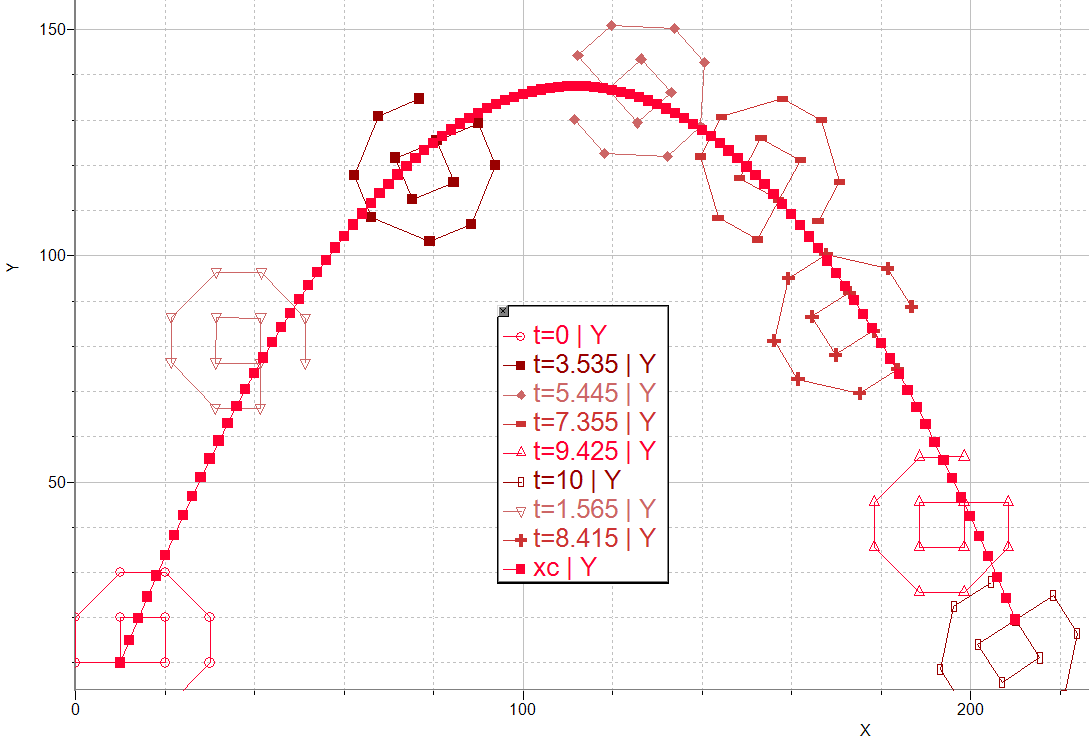
\includegraphics[width=\linewidth]{Pictures/xki_parabolic_12points.png}
  \caption{Пример расчета движения точек твердого тела}
  \label{fig:xki}
\end{figure}
\\Для более наглядной визуализации результатов расчет была реализована программа на языке программирования Python, которая создает анимацию движения твердого тела по предрассчитанным данным о положениях точек.
Результат работы данной программы прилагается в файле TestMovement.gif.

\subsection{Исследование сходимости}
Для расчета ошибки численного моделирования в данном примере было вычислено аналитическое решение.\\
Ошибка была рассчитана по норме $l_2$: как среднеквадратичное отклонение по следующей формуле:
\[
error_k=\sqrt{\sum_{i=0}^{stepN}||\overrightarrow{x}_k^i-\overrightarrow{x_{real}}_k^i||^2}
\]
Где $\overrightarrow{x_{real}}_k^i$ – положение k-ой точки твердого тела в момент времени $t=i\Delta t$, полученное из аналитического решения.\\
Ошибка расчета $\overrightarrow{x}_c$ - центра твердого тела:\\
Среднеквадратичное отклонение при вычислении 4000 шагов на отрезке времени 10с (длина временного шага 0.0025) составляет 2.47756e-10.\\
Ошибка расчета $\overrightarrow{x}_3$:\\
Среднеквадратичное отклонение при вычислении 4000 шагов на отрезке времени 10с (длина временного шага 0.0025) составляет 0.000469316.\\
Следует отметить сходимость рассчитанного решения к аналитическому: при измельчении шага $\Delta x$, значение ошибки $error_k$ стремится к 0:\\
\begin{figure}[h!]
  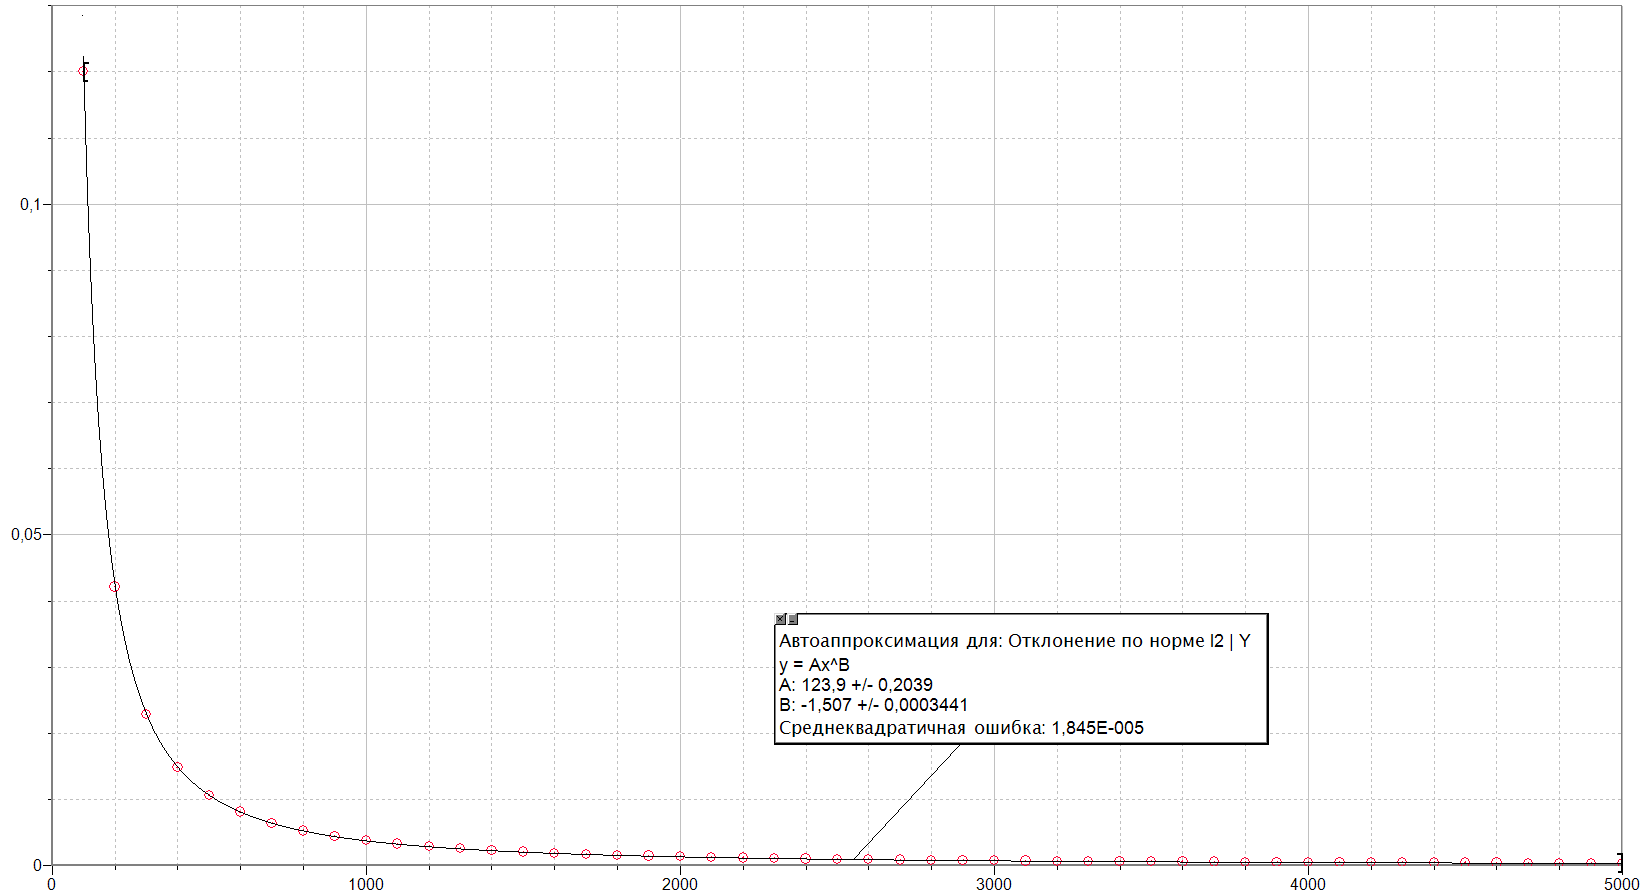
\includegraphics[width=\linewidth]{Pictures/dm_error_convergence.png}
  \caption{Сходимость метода DM. Среднеквадратичное отклонение при измельчении шага по времени}
  \label{fig:dm_err}
\end{figure}
.\\

\section{Численное решение уравнения переноса в одномерном случае со стационарным полем скоростей}
\subsection{Постановка задачи}
Теперь обратимся к решению уравнения переноса.
Данное уравнение в частных производных представлено в следующем виде:
\[
\frac{\partial f}{\partial t}+\nabla\cdot(\overrightarrow{u}f)-f\nabla\cdot\overrightarrow{u}=0
\]
Где $\overrightarrow{u}$ – векторное поле скоростей, $f$ - переносимая скалярная величина. Определим  как функцию Хевисайда, принимающую значения 0 и 1:
\begin{equation}
f(x,t)=\begin{cases}1 & {\bf x}\not\in D(t) \\0 & {\bf x}\in D(t)\end{cases}
\end{equation}
$\nabla$ – оператор дивергенции.\\
В одномерном случае данная задача рассматривается в виде:
\[
\frac{\partial f}{\partial t}+\frac{\partial }{\partial x}(uf)-f\frac{\partial u}{\partial x}=0
\]
Также мы предполагаем, что поле скоростей  соленоидально, то есть $\nabla\cdot u=0$. В этом случае задача рассматривается в виде:
\[
\frac{\partial f}{\partial t}+u\frac{\partial f}{\partial x}=0
\]
Начальные условия для уравнения переноса:
\begin{itemize}
	\item {Постоянное и положительное поле скоростей $\overrightarrow{u}$}
	\item Начальное распределение характеристической функции $f\mid_{t=0}=f(x,0)$
\end{itemize}
Необходимо найти:\\
Характеристическую функцию $f$ в исследуемой области $D$ на отрезке времени $[0; T]$.

\subsection{Численное решение}

\paragraph{Дискретизация.}
Отрезок $[0;X]$, на котором рассматривается данное уравнение, разбивается на $cellCount$ последовательных подотрезков, длиной $\Delta x_i$ каждый – ячейки сетки. i=1..cellCount. Положения $x_{i-\frac{1}{2}}$, $x_{i+\frac{1}{2}}$ являются узлами данной сетки (ребрами ячеек). $\Delta x_i=x_{i+\frac{1}{2}}-x_{i-\frac{1}{2}}$. Для реализации программы была выбрана равномерная сетка с ячейками равной длины $\Delta x$. Зададим длину временного шага $\Delta t$ и построим схему для вычисления средних значений функции $f(x,t)$ в каждой ячейке.\\

\begin{equation}
\overline{f}_i^n=\frac{1}{\Delta x_i}\int_{x_{i-\frac{1}{2}}}^{x_{i+\frac{1}{2}}}f(x,t_n)dx 
\end{equation}
- среднее по ячейке значение функции $f(x,t)$ на i-ом отрезке $\Delta x_i$ на n-ом временном шаге. В дальнейшем будем обозначать его как просто $f_i^n$.\\
$u$ - скорость в каждой ячейке исследуемой области (для твердого тела) на каждом шаге по времени (постоянное положительное поле скоростей).

\paragraph{Численное решение.}
Рассмотрим уравнение переноса в одномерном случае и при постоянной положительной скорости:
\[
\frac{\partial f}{\partial t}+u\frac{\partial f}{\partial x}=0
\]
После интегрирования данного уравнения по времени на временном шаге $[t_n; t_{n+1}]$:
\[
(f^{n+1}-f^n)+u\int_{t_n}^{t_{n+1}}\frac{\partial f}{\partial x} dt=0
\]
Представим производную $\frac{\partial f}{\partial x}$ в виде разностной схемы первого порядка:
\[
\frac{\partial f}{\partial x}=\frac{f_{i+\frac{1}{2}}-f_{i-\frac{1}{2}}}{\Delta x}
\]
Для приближенного вычисления интеграла $\int_{t_n}^{t_{n+1}}F dt$ используем квадратурную формулу прямоугольников:
\[
\int_{t_n}^{t_{n+1}}F dt=F^{n+\frac{1}{2}}\Delta t
\]
После подстановки уравнение примет следующий вид:
\[
f_i^{n+1}-f_i^n+\frac{u\Delta t}{\Delta x}(f_{i+\frac{1}{2}}^{n+\frac{1}{2}}-f_{i-\frac{1}{2}}^{n+\frac{1}{2}})=0
\]
Таким образом, значения характеристической функции $f_i^{n+1}$ на следующем временном шаге определяются как:
\[
f_i^{n+1}=f_i^n-\frac{u\Delta t}{\Delta x}(f_{i+\frac{1}{2}}^{n+\frac{1}{2}}-f_{i-\frac{1}{2}}^{n+\frac{1}{2}})
\]
Значения $f_i^n$ известны на каждом временном шаге, а для вычисления значений $f_{i+\frac{1}{2}}^{n+\frac{1}{2}}, f_{i-\frac{1}{2}}^{n+\frac{1}{2}}$ используем интерполяционную функцию $\Psi$:
\[
f_{i+\frac{1}{2}}^{n+\frac{1}{2}}=\Psi_i(x_{i+\frac{1}{2}}-u\frac{\Delta t}{2})
\]
\[
f_{i-\frac{1}{2}}^{n+\frac{1}{2}}=\Psi_{i-1}(x_{i-\frac{1}{2}}-u\frac{\Delta t}{2})
\]
Функция $\Psi_i(x)$ строится на каждой ячейке, а $\Psi_{i-1}(x)$ берется из предыдущей ячейки. Конкретное значение интерполяционной функции $\Psi_i(x)$ зависит от выбора схемы или комбинации схем численного решения.

\section{Численное решение уравнения переноса в одномерном случае с нестационарным полем скоростей}
Уравнение переноса в общем случае имеет следующий вид:
\begin{equation}
\label{eqn:TE}
\frac{\partial f}{\partial t}+\nabla\cdot(f\overrightarrow{u})=0
\end{equation}
Где u – векторное поле скоростей, f - переносимая скалярная величина, $ \nabla $ – оператор дивергенции. Определим f как функцию Хевисайда, принимающую значения 0 и 1:
\begin{equation}
f(x,t)=\begin{cases}1 & {\bf x}\in liquid \\0 & {\bf x}\not\in liquid\end{cases}
\end{equation}
В одномерном случае уравнение сводится к виду:
\begin{equation}
\label{eqn:TE1D}
\frac{\partial f}{\partial t} + \frac{\partial (f u)}{\partial x}=0
\end{equation}

\subsection{Численное решение}
\label{sec:TESolutionUnonstat}
\paragraph{Дискретизация.}
Для численного решения проводится дискретизация:

Отрезок $[0;X]$, на котором рассматривается данное уравнение, разбивается на $cellCount$ последовательных подотрезков, длиной $\Delta x_i$ каждый – ячейки сетки. i=1..cellCount. Положения $x_{i-\frac{1}{2}}$, $x_{i+\frac{1}{2}}$ являются узлами данной сетки (ребрами ячеек). $\Delta x_i=x_{i+\frac{1}{2}}-x_{i-\frac{1}{2}}$. Для реализации программы была выбрана равномерная сетка с ячейками равной длины $\Delta x$. Зададим длину временного шага $\Delta t$ и построим схему для вычисления средних значений функции $f(x,t)$ в каждой ячейке.
\begin{equation}
\overline{f}_i^n=\frac{1}{\Delta x_i}\int_{x_{i-\frac{1}{2}}}^{x_{i+\frac{1}{2}}}f(x,t_n)dx 
\end{equation}
- среднее по ячейке значение функции $f(x,t)$ на i-ом отрезке $\Delta x_i$ на n-ом временном шаге. В дальнейшем будем обозначать его как просто $f_i^n$.

\paragraph{Численное решение в общем случае.}
Проинтегрируем уравнение переноса в одномерном случае (\ref{eqn:TE1D}) по времени на шаге $[t_n; t_{n+1}]$:
\[
(f^{n+1}-f^n)+\int_{t_n}^{t_{n+1}}\frac{\partial(f u)}{\partial x}d\tau=0
\]
Для численного дифференцирования используем явную разностную схему 2 порядка:
\[
\frac{\text{d}(f u)}{\text{d}x}=\frac{f_{i+\frac{1}{2}}u_{i+\frac{1}{2}}-f_{i-\frac{1}{2}}u_{i-\frac{1}{2}}}{\Delta x_i}
\]
В результате уравнение переноса преобразуется к виду:
\begin{equation}
\label{eqn:TE1DdiffScheme}
(f_i^{n+1}-f_i^n)
+
\frac{1}{\Delta x_i}
\int_{t_n}^{t_{n+1}}
f_{i+\frac{1}{2}}u_{i+\frac{1}{2}}d\tau
-
\frac{1}{\Delta x_i}
\int_{t_n}^{t_{n+1}}
f_{i-\frac{1}{2}}u_{i-\frac{1}{2}} d\tau
=0
\end{equation}

\paragraph{Численное решение для нестационарного поля скоростей твердого тела.}
Перепишем уравнение (\ref{eqn:TE1DdiffScheme}), полученное для произвольного поля скоростей, для поля скоростей твердого тела:
\[
(f_i^{n+1}-f_i^n)
+
\frac{1}{\Delta x_i} (
\int_{t_n}^{t_{n+1}}
{u}f_{i+\frac{1}{2}}d\tau
-
\int_{t_n}^{t_{n+1}}
{u}f_{i-\frac{1}{2}}d\tau
)=0
\]
Интегралы
\begin{equation}
\label{eqn:FlowR}
\Phi_{i+\frac{1}{2}}=\int_{t_n}^{t_{n+1}}
{u}f_{i+\frac{1}{2}}d\tau
\end{equation}
\begin{equation}
\label{eqn:FlowL}
\Phi_{i-\frac{1}{2}}\int_{t_n}^{t_{n+1}}
{u}f_{i-\frac{1}{2}}d\tau
\end{equation}
представляют собой потоки через правую $x_{i+\frac{1}{2}}=x_R$ и левую $x_{i-\frac{1}{2}}=x_L$ грани ячейки $\Delta x_i = \Delta x$ соответственно.\\

Для вычисления значений $f_{x^*}^{t^*}$ необходимо построить подсеточную реконструкцию решения на соответствующей ячейке. При таком подходе значения $f_{x^*}^{t^*}$ считаются как значения интерполяционной функции, соответствующей методу решения.
\[
f_{x^*}^{t^*} = \Psi_0(x^*, t^*)
\]
Интерполяционная функция $\Psi_0(x^*, t^*)$ :
\begin{equation}
\label{eqn:PsyIntrpolationFunc}
\Psi_0(x^*, t^*) = \begin{cases}
\Psi_{L}(x(x^*,\tau^*))
& \int_{t_n}^{t_{n+1}} u^{\tau}d\tau\geq0
\\
\Psi_{R}(x(x^*,\tau^*))
& \int_{t_n}^{t_{n+1}} u^{\tau}d\tau < 0
\end{cases}
\end{equation}
Таким образом, реализуется метод \textit{upwind}: расчета потоков через грани по направлению переноса.
То есть, при вычислении потока $\Phi_{x^*}$ для положительной скорости $u$ переноса на грани $x^*$ ячейки в течение шага $[t_n; t_{n+1}]$, будет использована интерполяционная функция $\Psi_{j}(x(x^*,\tau^*))$, построенная на ячейке $j$ слева от данной грани $x^*$, а при вычислении потока для отрицательной скорости $u$ будет использована интерполяционная функция $\Psi_{j}(x(x^*,\tau^*))$, построенная на ячейке $j$ справа от данной грани $x^*$.\\

В дальнейшем для выбора интерполяционной функции $\Psi_{j}$ в исследовании будут рассмотрены такие методы, как метод MUSCL (линейная интерполяция), метод THINC (интерполяция гиперболическим тангенсом) и метод Jump Reconstruction (интерполяция скачком).\\

Выражение для расчета объемной доли переносимой скалярной величины через потоки в ячейке $\Delta x_i$ на следующем временном шаге $t_{n+1}$ имеет вид:
\begin{equation}
\label{fiNextFlows}
f_i^{n+1}=f_i^n
-
\frac{1}{\Delta x_i} (
\Phi_{i+\frac{1}{2}}
-
\Phi_{i-\frac{1}{2}}
)=0
\end{equation}

\subsection{Метод характеристик}
Интерполяционные функции $\Psi_i(x)$ - функции координаты. Для интегрирования по времени необходимо представить их как функции времени. Для этого был использован метод характеристик. Данный метод позволяет определить линии в плоскости $(x, t)$, вдоль которых решение постоянно. Это позволяет доставить решение, выходящее из заданного положения $(x(t), t_n)$ в определенную точку $(x^*, t_n+\tau^*)$ в пространстве $(x, t)$. таким образом, появляется возможность вместо координаты $x$, в качестве аргумента интерполяционной функции $\Psi_i(x)$ использовать функцию времени $x(t)$.

Рассмотрим решение уравнения переноса с помощью метода характеристик.
\begin{equation}
\frac{\text{d}f}{\text{d}t} + \frac{\text{d}(f u)}{\text{d}x}=0
\end{equation}
Нам бы хотелось свести это дифференциальное уравнение в частных производных первого порядка к обыкновенному дифференциальному уравнению вдоль соответствующей кривой, то есть получить уравнение вида:
\[
\frac{\text{d}}{\text{d}s}f(x(s),t(s))=F(f,x(s),t(s))
\]
где кривая $(x(s),t(s))$ — характеристика.\\
Установим, что
\begin{equation}
\label{eqn:CharacteristicsMethodEq}
\frac{\text{d}}{\text{d}s}f(x(s),t(s))=\frac{\partial f}{\partial x}\frac{\text{d}x}{\text{d}s}+\frac{\partial f}{\partial t}\frac{\text{d}t}{\text{d}s}
\end{equation}
Положим, что
\[
\frac{\text{d}t}{\text{d}s}=1
\]
Следовательно, при $t(0)=0$, $s=t$. И теперь будем составлять ОДУ, используя метод характеристик в виде:
\[
\frac{\text{d}}{\text{d}t}f(x(t),t)=F(f,x(t),t)
\]
Будем искать решение вдоль характеристик, уравнение которых имеет вид:
\[
\frac{\text{d}x}{\text{d}t}=u(t)
\]
В таком случае уравнение (\ref{eqn:CharacteristicsMethodEq}) можно переписать в виде:
\[
\frac{\text{d}}{\text{d}t}f(x(t),t)=u(t)\frac{\partial f}{\partial x}+\frac{\partial f}{\partial t}
\]
таким образом, вдоль характеристики $(x(t),t)$ исходное уравнение в частных производных превращается в ОДУ:
\[
f'_t=F(f,x(t),t)=0
\]
Данное уравнение говорит о том, что вдоль характеристик решение постоянное. Таким образом, $f(x,t)=f(x_0,0)$, где точки $(x,t)$ и $(x_0,0)$ лежат на одной характеристике. Видно, что для нахождения общего решения достаточно найти характеристики уравнения в виде:
\begin{equation}
\label{eqn:CharacteristicsEq}
\frac{\text{d}x}{\text{d}t}=u(t)
\end{equation}
Будем искать решение на временном слое $t_n$.
\\$\tau$ - время на слое $[t_n; t_{n+1}]$. То есть $\tau=0 \Leftrightarrow t=t_n$, $\tau=\Delta t \Leftrightarrow t=t_{n+1}$.
\\Проинтегрируем уравнение (\ref{eqn:CharacteristicsEq}) по $t$ от $t_n$ до $t_n+\tau$:
\begin{equation}
\label{eqn:CommonCharacteristics}
x(t_n+\tau)-x(t_n)=\int_{t_n}^{t_n+\tau}u(t)dt + C
\end{equation}
Что является общим видом характеристической функции для данного уравнения в частных производных.
\\Найдем такую характеристику, которая в момент времени $\tau^*$ проходила через точку $x^*$. Подставим в характеристическую функцию (\ref{eqn:CommonCharacteristics}) данные начальные условия:
\[
x(t_n+\tau^*)-x(t_n)=\int_{t_n}^{t_n+\tau^*}u(t)dt + C^*
\]
Тогда
\[
C^* = x^*-x(t_n)-\int_{t_n}^{t_n+\tau^*}u(t)dt
\]
Подставим $C^*$ обратно в общий вид уравнения характеристической функции (\ref{eqn:CommonCharacteristics}), чтобы получить характеристику:
\[
x(t_n+\tau)-x(t_n)=\int_{t_n}^{t_n+\tau}u(t)dt + x^*-x(t_n)-\int_{t_n}^{t_n+\tau^*}u(t)dt
\]
\begin{equation}
\label{eqn:Characteristic}
x(t_n+\tau)=\int_{t_n}^{t_n+\tau}u(t)dt + x^*-\int_{t_n}^{t_n+\tau^*}u(t)dt
\end{equation}
Узнаем координату, из которой выходила данная характеристика в момент времени $\tau=0$:
\[
x\mid_{\tau=0}=\int_{t_n}^{t_n}u(t)dt + x^*-\int_{t_n}^{t_n+\tau^*}u(t)dt
\]
\begin{equation}
\label{eqn:CharacteristicFromZero}
x\mid_{\tau=0}=x^*-\int_{t_n}^{t_n+\tau^*}u(t)dt
\end{equation}
Данное значение необходимо использовать как аргумент интерполяционной функции (\ref{eqn:PsyIntrpolationFunc}).

\subsection{Аппроксимация интегралов}
В зависимости от выбранного метода подсеточной реконструкции, интегралы в потоках и в характеристике могут быть вычислены приближенно, с использованием квадратурных формул в случае непрерывной интерполяции распределения (этот способ использовался для методов MUSCL и THINC), или точно в случае кусочно-постоянной интерполяции распределения (этот способ использовался для метода JR).
\paragraph{Непрерывное распределение.}
Рассмотрим непрерывную реконструкцию распределения. Для вычисления интегралов была использована квадратурная формула трапеции.\\
Интеграл в характеристике (\ref{eqn:CharacteristicFromZero}) был заменен на квадратурную формулу:
\begin{equation}
\label{eqn:CharacteristicQuadr}
x\mid_{\tau=0}=x^*-\int_{t_n}^{t_n+\tau^*}u(t)dt=x^*-\Delta t \frac{u(t_n)+u(t_n+\tau^*)}{2}
\end{equation}
Для аппроксимации интегралов потоков (\ref{eqn:FlowR}), (\ref{eqn:FlowL}) была использована квадратурная формула трапеции.\\
Интегралы в потоках были заменены на квадратурные формулы:
\begin{equation}
\label{eqn:flowRQuadr}
\Phi_{i+\frac{1}{2}}=\int_{t_n}^{t_{n+1}}
{u}f_{i+\frac{1}{2}}d\tau= \frac{\Delta t}{2}(
u^{n+1}f_{i+\frac{1}{2}}^{n+1} +
u^{n}f_{i+\frac{1}{2}}^{n}
)
\end{equation}
\begin{equation}
\label{eqn:flowLQuadr}
\Phi_{i-\frac{1}{2}}=\int_{t_n}^{t_{n+1}}
{u}f_{i-\frac{1}{2}}d\tau= \frac{\Delta t}{2}(
u^{n+1}f_{i-\frac{1}{2}}^{n+1} +
u^{n}f_{i-\frac{1}{2}}^{n}
)
\end{equation}

Таким образом, значения потоков (\ref{eqn:FlowR}), (\ref{eqn:FlowL}) будут иметь вид:
\begin{equation}
\label{eqn:FlowRContPsi}
\Phi_{i+\frac{1}{2}}= \frac{\Delta t}{2}(
u^{n} \Psi_{0}(x(x_{i+\frac{1}{2}}, 0))
+
u^{n+1} \Psi_{0}(x(x_{i+\frac{1}{2}}, \Delta t))
)
\end{equation}
\begin{equation}
\label{eqn:FlowLContPsi}
\Phi_{i-\frac{1}{2}}= \frac{\Delta t}{2}(
u^n \Psi_{0}(x(x_{i-\frac{1}{2}}, 0))
+
u^{n+1} \Psi_{0}(x(x_{i-\frac{1}{2}}, \Delta t))
)
\end{equation}
Подставляя в них характеристики с координатами соответствующих граней и с нужным шагом по времени, получим окончательный вид уравнений для расчета потоков:
\begin{equation}
\label{eqn:FlowRContPsi}
\Phi_{i+\frac{1}{2}}= \frac{\Delta t}{2}(
u^{n} \Psi_{0}(x_R)
+
u^{n+1} \Psi_{0}(x^R-\Delta t \frac{u^n+u^{n+1}}{2}))
)
\end{equation}
\begin{equation}
\label{eqn:FlowLContPsi}
\Phi_{i-\frac{1}{2}}= \frac{\Delta t}{2}(
u^{n} \Psi_{0}(x_L)
+
u^{n+1} \Psi_{0}(x^L-\Delta t \frac{u^n+u^{n+1}}{2}))
)
\end{equation}

\paragraph{Кусочно - постоянное распределение. Метод JR.}\label{sec:JR_flows}
В силу кусочно - постоянного характера распределения при использовании подхода аппроксимации скачка разрывной функцией (Jump Reconstruction), для данного метода необходим точный расчет интегралов. Найти аналитическое решение в данном случае возможно из-за того же кусочно - постоянного характера распределения.\\
Рассмотрим случай положительной скорости на временном шаге $[t_n; t_{n+1}]$: $u^n+u^{n+1}\geq 0$. Случай отрицательной скорости рассматривается аналогично.\\
Интеграл в характеристике (\ref{eqn:CharacteristicFromZero}) также был заменен на квадратурную формулу:
\begin{equation}
x\mid_{\tau=0}=x^*-\int_{t_n}^{t_n+\tau^*}u(t)dt=x^*-\Delta t u^n
\end{equation}
Подставляя данную формулу в уравнения потоков (\ref{eqn:FlowR}), (\ref{eqn:FlowL}), получим
\begin{equation}
\label{eqn:flowRJR}
\Phi_{i+\frac{1}{2}}=
\int_{t_n}^{t_{n+1}}{u}f_{i+\frac{1}{2}}d\tau=
\int_{t_n}^{t_{n+1}}u\Psi_{0}(x(x_{i+\frac{1}{2}}, \tau))d\tau=
u^{n+\frac{1}{2}}\int_{t_n}^{t_{n+1}}\Psi_{0}( x_{i+\frac{1}{2}}-\Delta t u^n )d\tau
\end{equation}
\begin{equation}
\label{eqn:flowLJR}
\Phi_{i-\frac{1}{2}}=
\int_{t_n}^{t_{n+1}}{u}f_{i-\frac{1}{2}}d\tau=
\int_{t_n}^{t_{n+1}}u\Psi_{0}(x(x_{i-\frac{1}{2}}, \tau))d\tau)=
u^{n+\frac{1}{2}}\int_{t_n}^{t_{n+1}}\Psi_{0}( x_{i-\frac{1}{2}}-\Delta t u^n )d\tau
\end{equation}
Метод Jump Reconstruction работает только на разрывных ячейках, поэтому построенная на разрывной ячейке функция $\Psi_i(x)$ будет иметь вид:
\[
\Psi_i(x)=\begin{cases}\Psi_+ & x\leq x^* \\ \Psi_- & x > x^*\end{cases}
\]
Где $x^*$ - положение разрыва в абсолютных координатах, введенных на сетке.\\
Таким образом, значения потоков (\ref{eqn:FlowR}), (\ref{eqn:FlowL}) будут иметь вид:
\begin{equation}
\label{eqn:FlowRJRPsiCase1}
\Phi_{i+\frac{1}{2}}=u^{n+\frac{1}{2}}(\Psi_i^+\tau^*+\Psi_i^-(\Delta t-\tau^*))
\end{equation}
\begin{equation}
\label{eqn:FlowLJRPsiCase1}
\Phi_{i-\frac{1}{2}}=u^{n+\frac{1}{2}}(\Psi_{i-1}^+\tau^*+\Psi_{i-1}^-(\Delta t-\tau^*))
\end{equation}
Где
\[
\tau^*=\frac{x_{i+\frac{1}{2}}-x_i^*}{u^n}
\]
Здесь предполагается, что $\tau^*\leq\Delta t$. В случае, если $\tau^*>\Delta t$, то
\begin{equation}
\label{eqn:FlowRJRPsiCase2}
\Phi_{i+\frac{1}{2}}=u^{n+\frac{1}{2}}\Psi_i^+\Delta t
\end{equation}
\begin{equation}
\label{eqn:FlowLJRPsiCase2}
\Phi_{i-\frac{1}{2}}=u^{n+\frac{1}{2}}\Psi_{i-1}^+\Delta t
\end{equation}
Оба случая можно объединить:
\begin{equation}
\label{eqn:FlowRJRPsi}
\Phi_{i+\frac{1}{2}}=u^{n+\frac{1}{2}}(\Psi_i^+min(\Delta t, \tau^*)+\Psi_i^-max(0, \Delta t-\tau^*))
\end{equation}
\begin{equation}
\label{eqn:FlowLJRPsi}
\Phi_{i-\frac{1}{2}}=u^{n+\frac{1}{2}}(\Psi_{i-1}^+min(\Delta t, \tau^*)+\Psi_{i-1}^-min(0, \Delta t-\tau^*))
\end{equation}

\section{Исследование различных схем}
Функция $\Psi_i(x)$ позволяет интерполировать значения на границах ячеек. Ее выбор определяет вид схемы численного решения: интерполяционной функции в точках разрыва функции – индикатора $f$, и, соответственно, вид получаемого решения. При выборе функции $\Psi(x)$ были рассмотрены следующие схемы:
\begin{itemize}
	\item Схема Годунова – схема кусочно-постоянной аппроксимации, имеет 1 порядок точности
	\item Схема MUSCL - монотонная восходящая схема для законов сохранения, имеет 2 порядок точности
	\item Схема THINC - гиперболический тангенс для отслеживания поверхности, позволяет существенно снизить эффект «численно вязкости», повышая, таким образом, точность решения.
	\item Схема JR - восполнение разрывной функцией, Jump Reconstruction
\end{itemize}

Схемы THINC и JR применяется только при выполнении определенных условий на значения  в ячейках сетки. Там, где эти условия не выполняются схему данные схемы комбинируют с другими схемами интерполяции, например со схемой Годунова или MUSCL.

\subsection{Метод Годунова(const)}
Схема Годунова - численная схема для решения дифференциальных уравнений в частных производных. Данная схема представляет собой консервативный метод конечных объемов, который решает точную или приближенную задачу Римана на границах между ячейками. Метод Годунова имеет точность первого порядка как в пространстве, так и во времени, но может использоваться в качестве базовой схемы для разработки схем более высокого порядка.

При реализации схемы Годунова в качестве функции $\Psi_i(x)$ берется константа – значение $f_i^n$ на том же временном шаге $t_n$ и в той же ячейке $\Delta x_i$.
\[
\Psi_i(x)=f_i
\]
Таким образом, общая формула расчета значений $f_i^{n+1}$ на следующем временном шаге представляет собой:
\[
f_i^{n+1}=f_i^n-\frac{u^n+u^{n+1}}{2}(f_i^n-f_{i-1}^n)\frac{\Delta t}{\Delta x}
\]
Результаты расчетов с помощью данного метода, после прохождения 1-6 периодов на разных сетках представлены ниже:
\\
\makebox[0pt][l]{%
\begin{minipage}{\textwidth}
\centering
    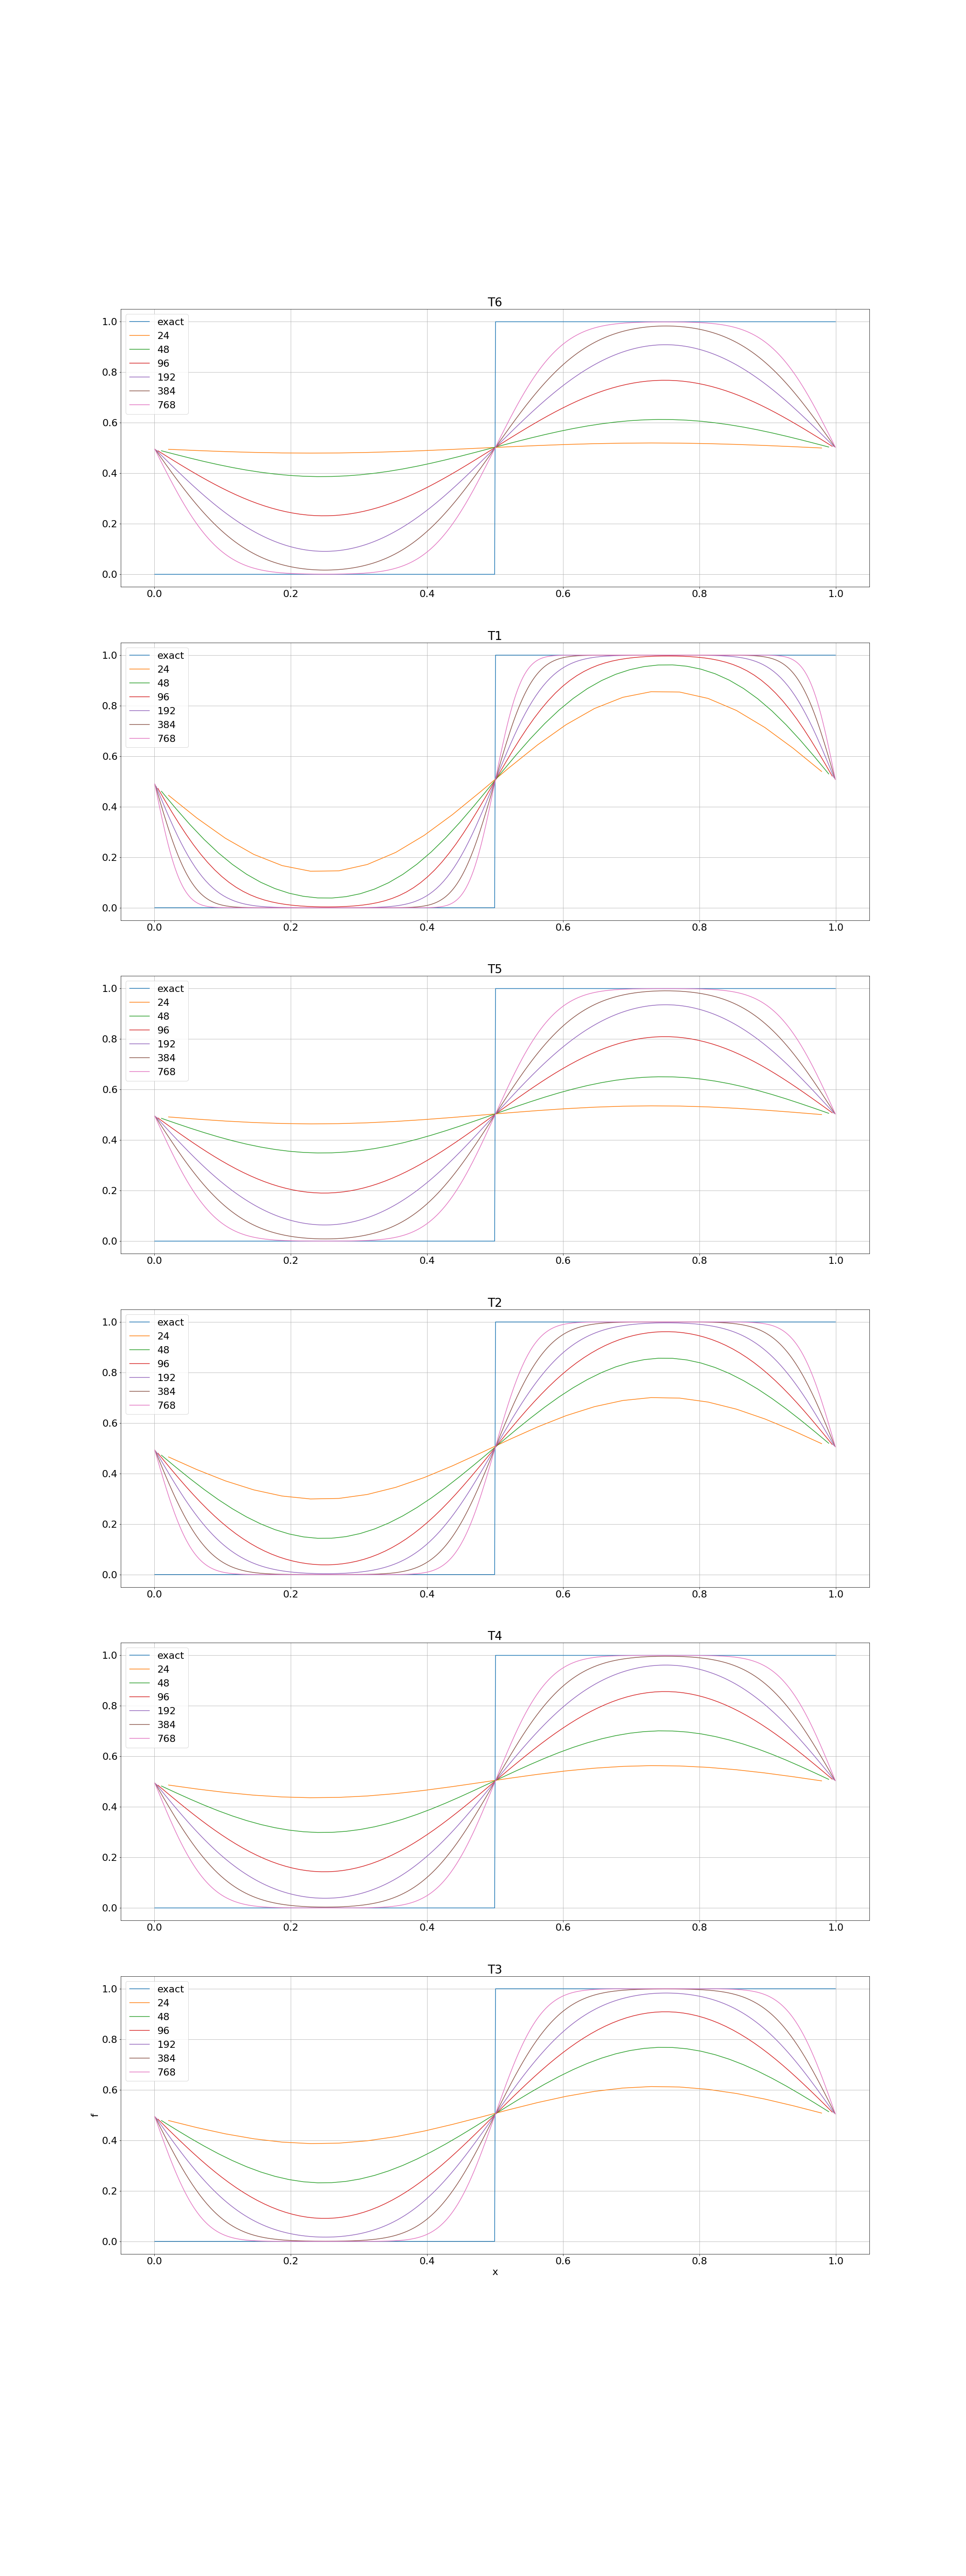
\includegraphics[width=0.5\linewidth]{Pictures/Godunov.png}
 \captionof{figure}{Расчеты 1D. Схема Годунова}
 \label{fig:Godunov}
\end{minipage}
}
\medskip
\\
Можно наблюдать значительное "размазывание" значений характеристической функции, которое увеличивается с каждым шагом по времени. Таким образом, проявляется эффект численной вязкости, который сильно искажает исходную форму твердого тела, представленного характеристической функцией.


\subsection{Метод MUSCL (linear)}
Схема MUSCL представляет собой метод конечных объемов и может применяться в случаях, когда система терпит разрывы. MUSCL - Monotonic Upstream-centered Scheme for Conservation Laws (Монотонная восходящая схема для законов сохранения). Данная схема имеет пространственную точность второго порядка. В отличие от схемы Годунова, для расчета потоков на границах ячеек используются не средние значения на ячейках, а значения линейных функций с ограничением наклона по левой и правой ячейке.

При реализации схемы MUSCL в качестве функции $\Psi_i(x)$ берется линейная функция, проходящая через центр ячейки – положение $x_i$, и имеющая угол наклона, равный значению  функции $minmod$ от $f_{iR}^n$ и $f_{iL}^n$.
\\
\makebox[0pt][l]{%
\begin{minipage}{\textwidth}
\centering
    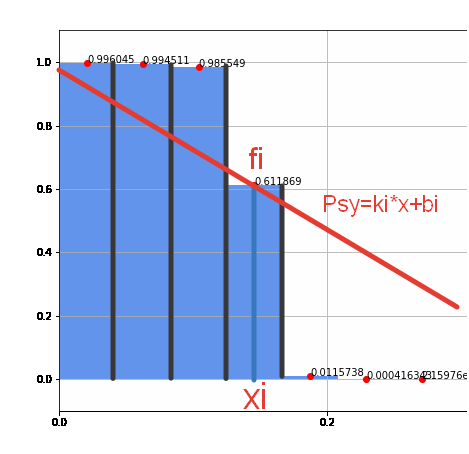
\includegraphics[width=0.6\linewidth]{Pictures/MUSCL_scheme.png}
 \captionof{figure}{Схема MUSCL}
 \label{fig:MUSCL_sheme}
\end{minipage}
}
\medskip
\[
\Psi_i(x)=k_i^nx+b_i^n
\]
Где
\[
k_i=minmod(f_{iR}^n, f_{iL}^n)
\]
\[
f_{iR}=\frac{f_{i+1}^n-f_i^n}{\Delta x}
\]
\[
f_{iL}=\frac{f_i^n-f_{i-1}^n}{\Delta x}
\]
\[
minmod(a, b) = \begin{cases}0 & ab<0\\ sgn(a)min(|a|,|b|) & ab \geq 0\end{cases}
\]
\[
b_i^n=f_i^n-k_i^nx_i
\]
Результаты расчетов с помощью данного метода, после прохождения 1-6 периодов на разных сетках представлены ниже:
\\
\makebox[0pt][l]{%
\begin{minipage}{\textwidth}
\centering
    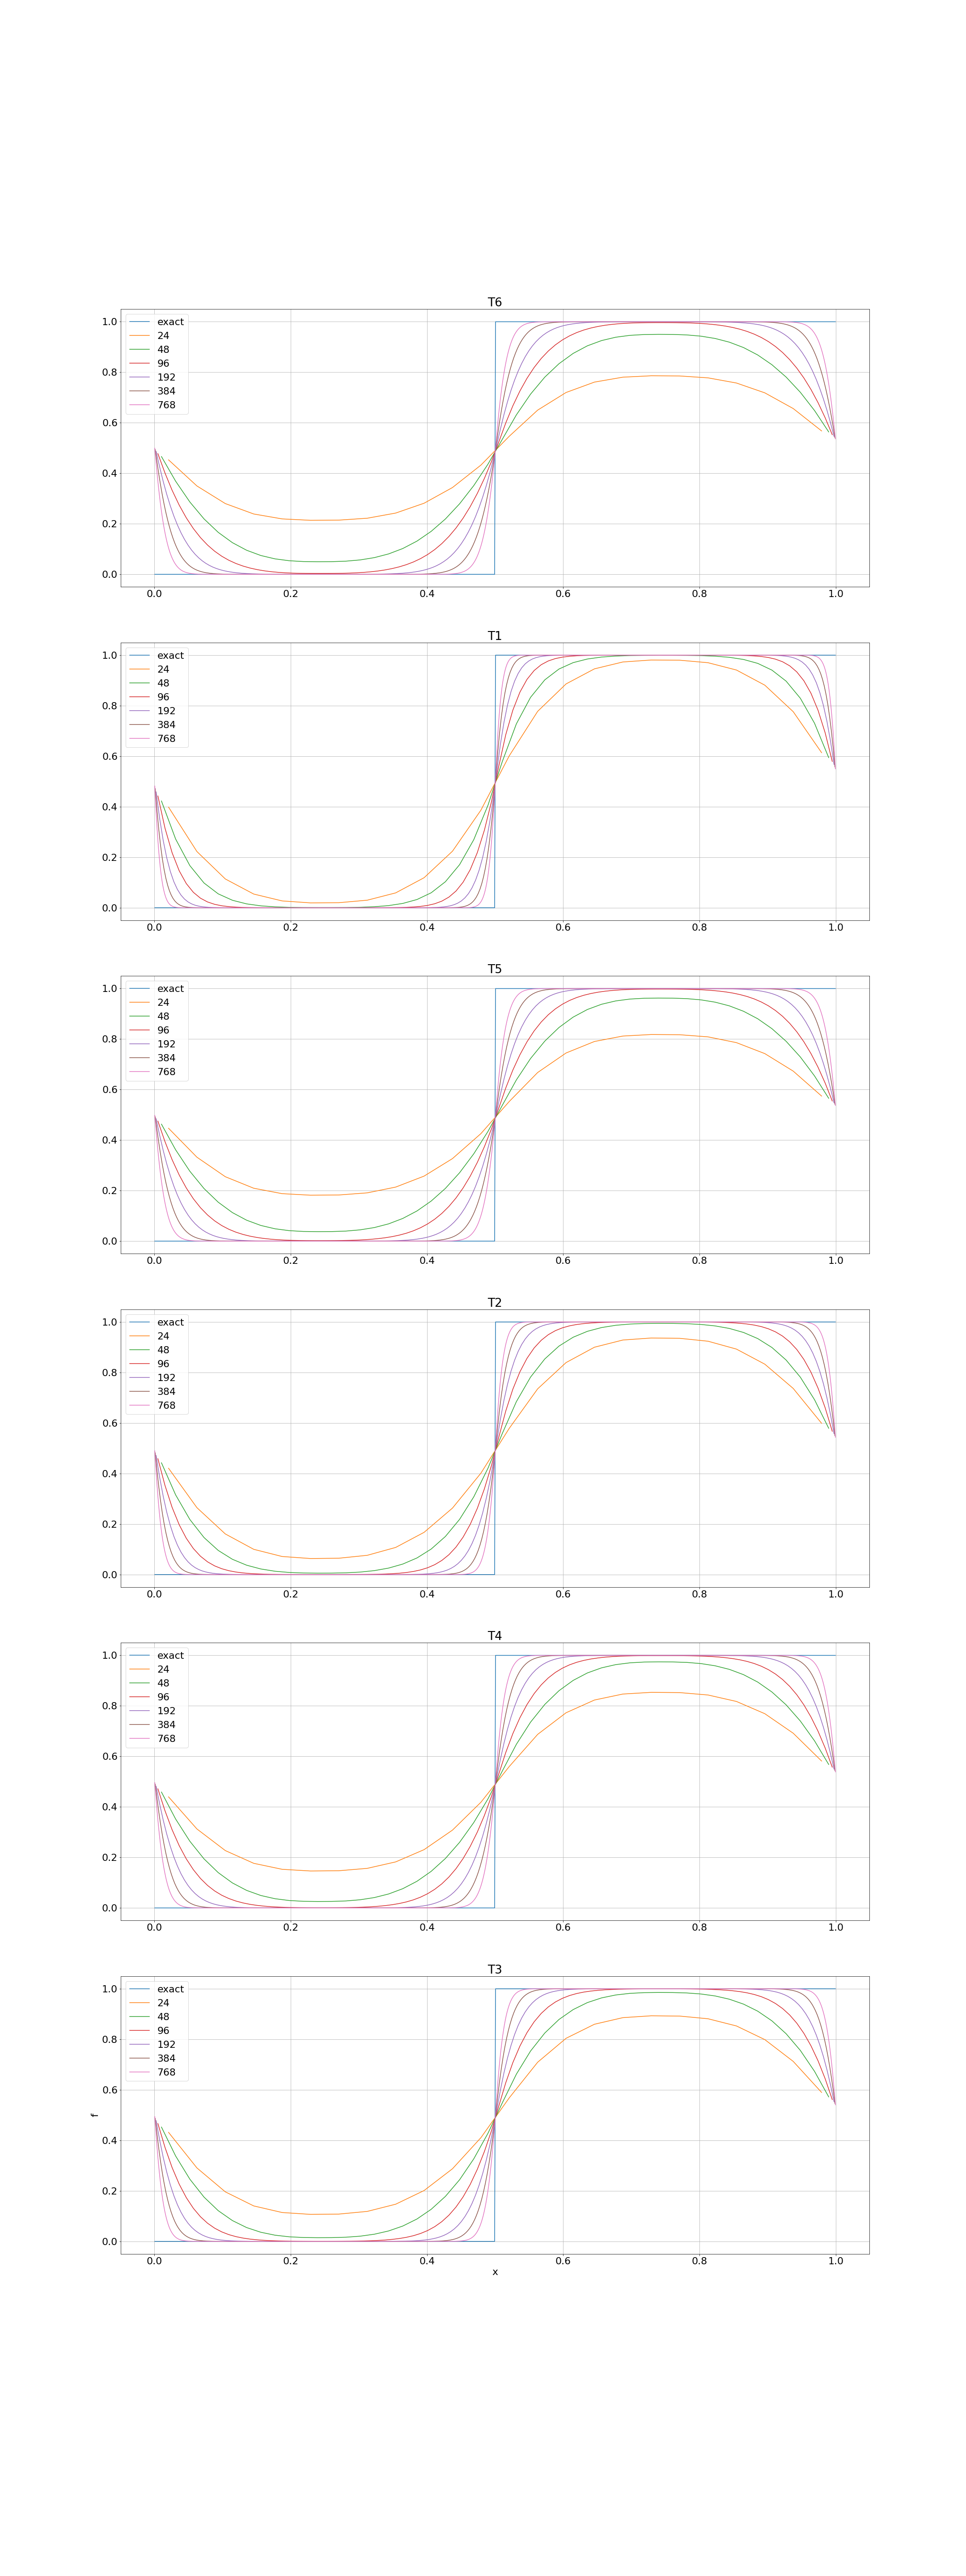
\includegraphics[width=0.5\linewidth]{Pictures/MUSCL.png}
 \captionof{figure}{Расчеты 1D. Схема MUSCL}
 \label{fig:MUSCL}
\end{minipage}
}
\medskip
\\
Можно видеть, что линейный метод MUSCL меньше "размазывает" значения характеристической функции по сравнению с постоянным восполнением метода Годунова.

\subsection{Метод THINC (tanh)}
Схема THINC - (tangent of hyperbola for interface capturing: гиперболический тангенс для отслеживания поверхности) представляет собой метод конечных объемов.

Данная схема применяется только в ячейках, где выполняется условие:
\[
\begin{cases}
\epsilon<f_i^n<1-\epsilon & \text{то есть, }f_i^n\in(0; 1)
\\
(f_{i+1}^n-f_i^n)(f_i^n-f_{i-1}^n) & \text{условие монотонности}
\end{cases}
\]
Где $\epsilon$ - малая величина. В расчетах использовалось значение $\epsilon=1e-4$.\\
В тех ячейках, где данное условие не выполняется, используется схема Годунова или MUSCL.\\
Для аппроксимации функции  на каждом  отрезке строится функция:
\[
F_i(x)=\frac{1}{2}(1+\gamma_itanh(\beta(\frac{x-x_{i-\frac{1}{2}}}{\Delta x}-x_i^*)))
\]
Где параметры $\beta$, $\gamma_i$ определяются следующим образом:
\[
\gamma_i=sgn(f_{i+1}^n-f_{i-1}^n)
\]
$\beta$ определяет сжатие по оси X – скорость прыжка.\\
Параметр $x_i^*$ – относительное расстояние до середины прыжка $f$ от левой границы отрезка $x_{i-\frac{1}{2}}$.
\\
\makebox[0pt][l]{%
\begin{minipage}{\textwidth}
\centering
    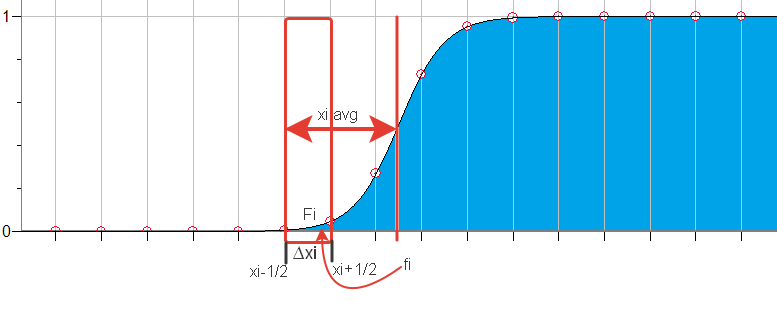
\includegraphics[width=\linewidth]{Pictures/THINC_scheme_xiavg.png}
 \captionof{figure}{Схема THINC. $x_i^*$.}
 \label{fig:THINC_scheme_xiavg}
\end{minipage}
}
\medskip
\\
Тогда интерполяционная функция для метода THINC строится нормировкой функции $F_i(x)$ на значения $f_{i\pm 1}^n$ следующим образом:
\[
\Psi_i(x)=f_{min}+F_i(x)\Delta f_i
\]
Где
\[
f_{min} = min(f_{i-1}^n, f_{i+1}^n)
\]
\[
f_{max} = max(f_{i-1}^n, f_{i+1}^n)
\]    
\[
\Delta f_i=f_{max}-f_{min}
\]
Здесь $F_i(x)$ - это функция гиперболического тангенса, аппроксимирующая f(x) на ячейке $\Delta x_i$.

$x_i^*$ определяется из интегрального уравнения:
\[
f_i^n=\frac{1}{\Delta x}\int_{x_{i-\frac{1}{2}}}^{x_{i+\frac{1}{2}}}\Psi_i(x)dx
\]
Аналитическое решение данного уравнения:
\[
f_i^n=\frac{1}{\Delta x}\int_{x_{i-\frac{1}{2}}}^{x_{i+\frac{1}{2}}}(f_{min}+
\frac{1}{2}(1+\gamma_itanh(\beta(\frac{x-x_{i-\frac{1}{2}}}{\Delta x}-x_i^*)))\Delta f_i)dx
\]
\[
x_i^*=\frac{1}{2\beta}log\left(\frac{exp(\frac{\beta}{\gamma_i}(1+\gamma_i-2\frac{f_i^n-f_{min}}{\Delta f_i}))-1}{1-exp(\frac{\beta}{\gamma_i}(1-\gamma_i-2\frac{f_i^n-f_{min}}{\Delta f_i}))}\right)
\]

Таким образом, общий алгоритм построения  на ячейке выглядит следующим образом:
\begin{enumerate}
\item По значениям $f_{i-1}^n$ и $f_{i+1}^n$ рассчитываются значения $\gamma_i$, $f_{min}$, $f_{max}$, $\Delta f_i$.
\item По значениям $\beta$, $gamma_i$, $f_i^n$, $f_{min}$, $\Delta f_i$ вычисляется значение $x_i^*$, необходимое для задания функции $F_i(x)$.
\item Теперь готово все необходимое для задания функции $\Psi_i(x)=f_{min}+F_i(x)\Delta f_i$ на отрезке $\Delta x_i$.
\end{enumerate}

Результаты расчетов с помощью комбинации схемы THINC и схемы Годунова, после прохождения 1-6 периодов на разных сетках представлены ниже:
\\
\makebox[0pt][l]{%
\begin{minipage}{\textwidth}
\centering
    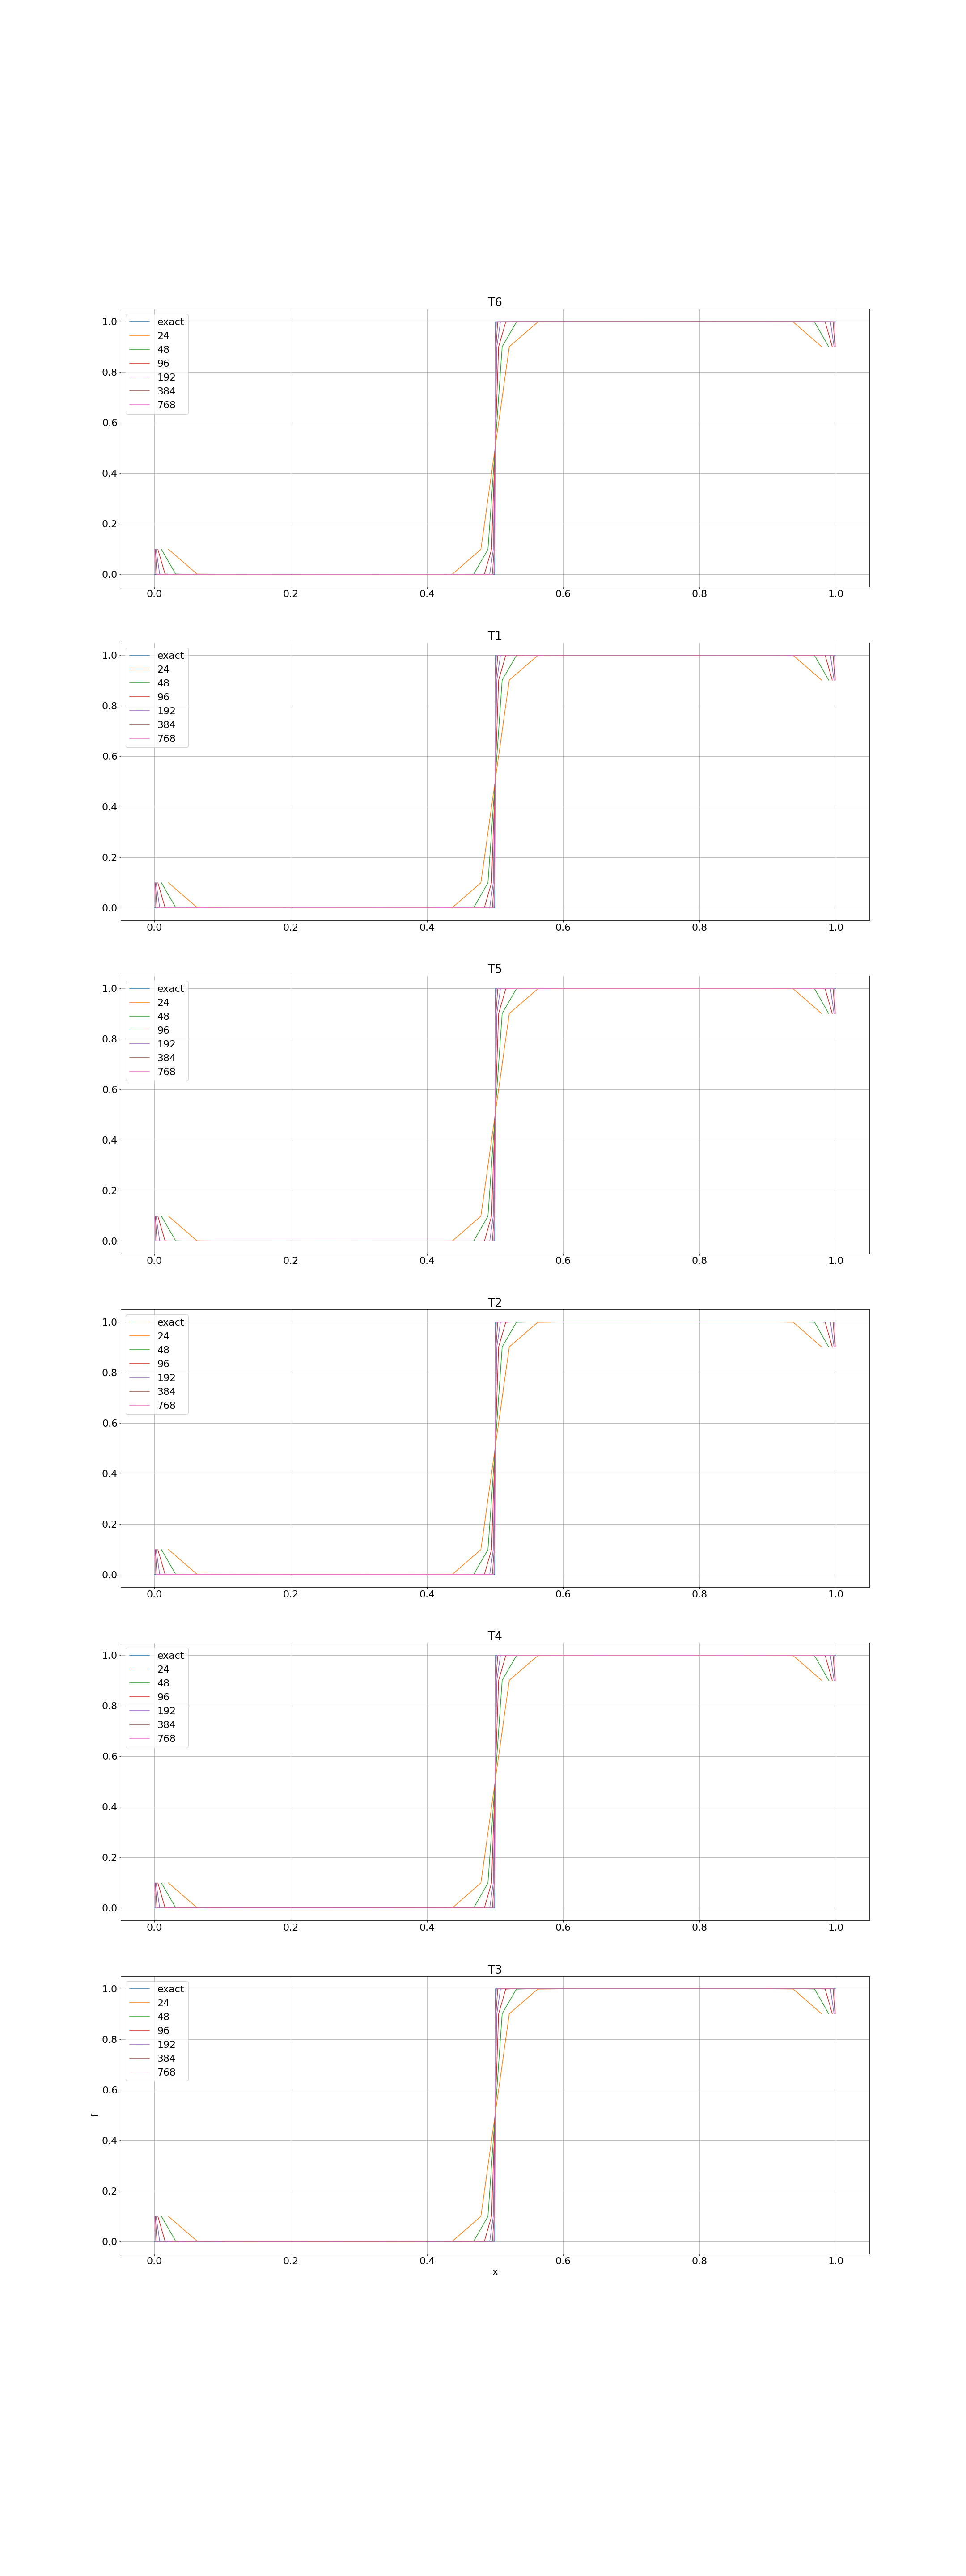
\includegraphics[width=0.5\linewidth]{Pictures/THINC_Godunov.png}
 \captionof{figure}{Расчеты 1D. Схема THINC + Годунов}
 \label{fig:THINC_Godunov}
\end{minipage}
}
\medskip
\\
Результаты расчетов с помощью комбинации схемы THINC и схемы MUSCL, после прохождения 1-6 периодов на разных сетках представлены ниже:
\\
\makebox[0pt][l]{%
\begin{minipage}{\textwidth}
\centering
    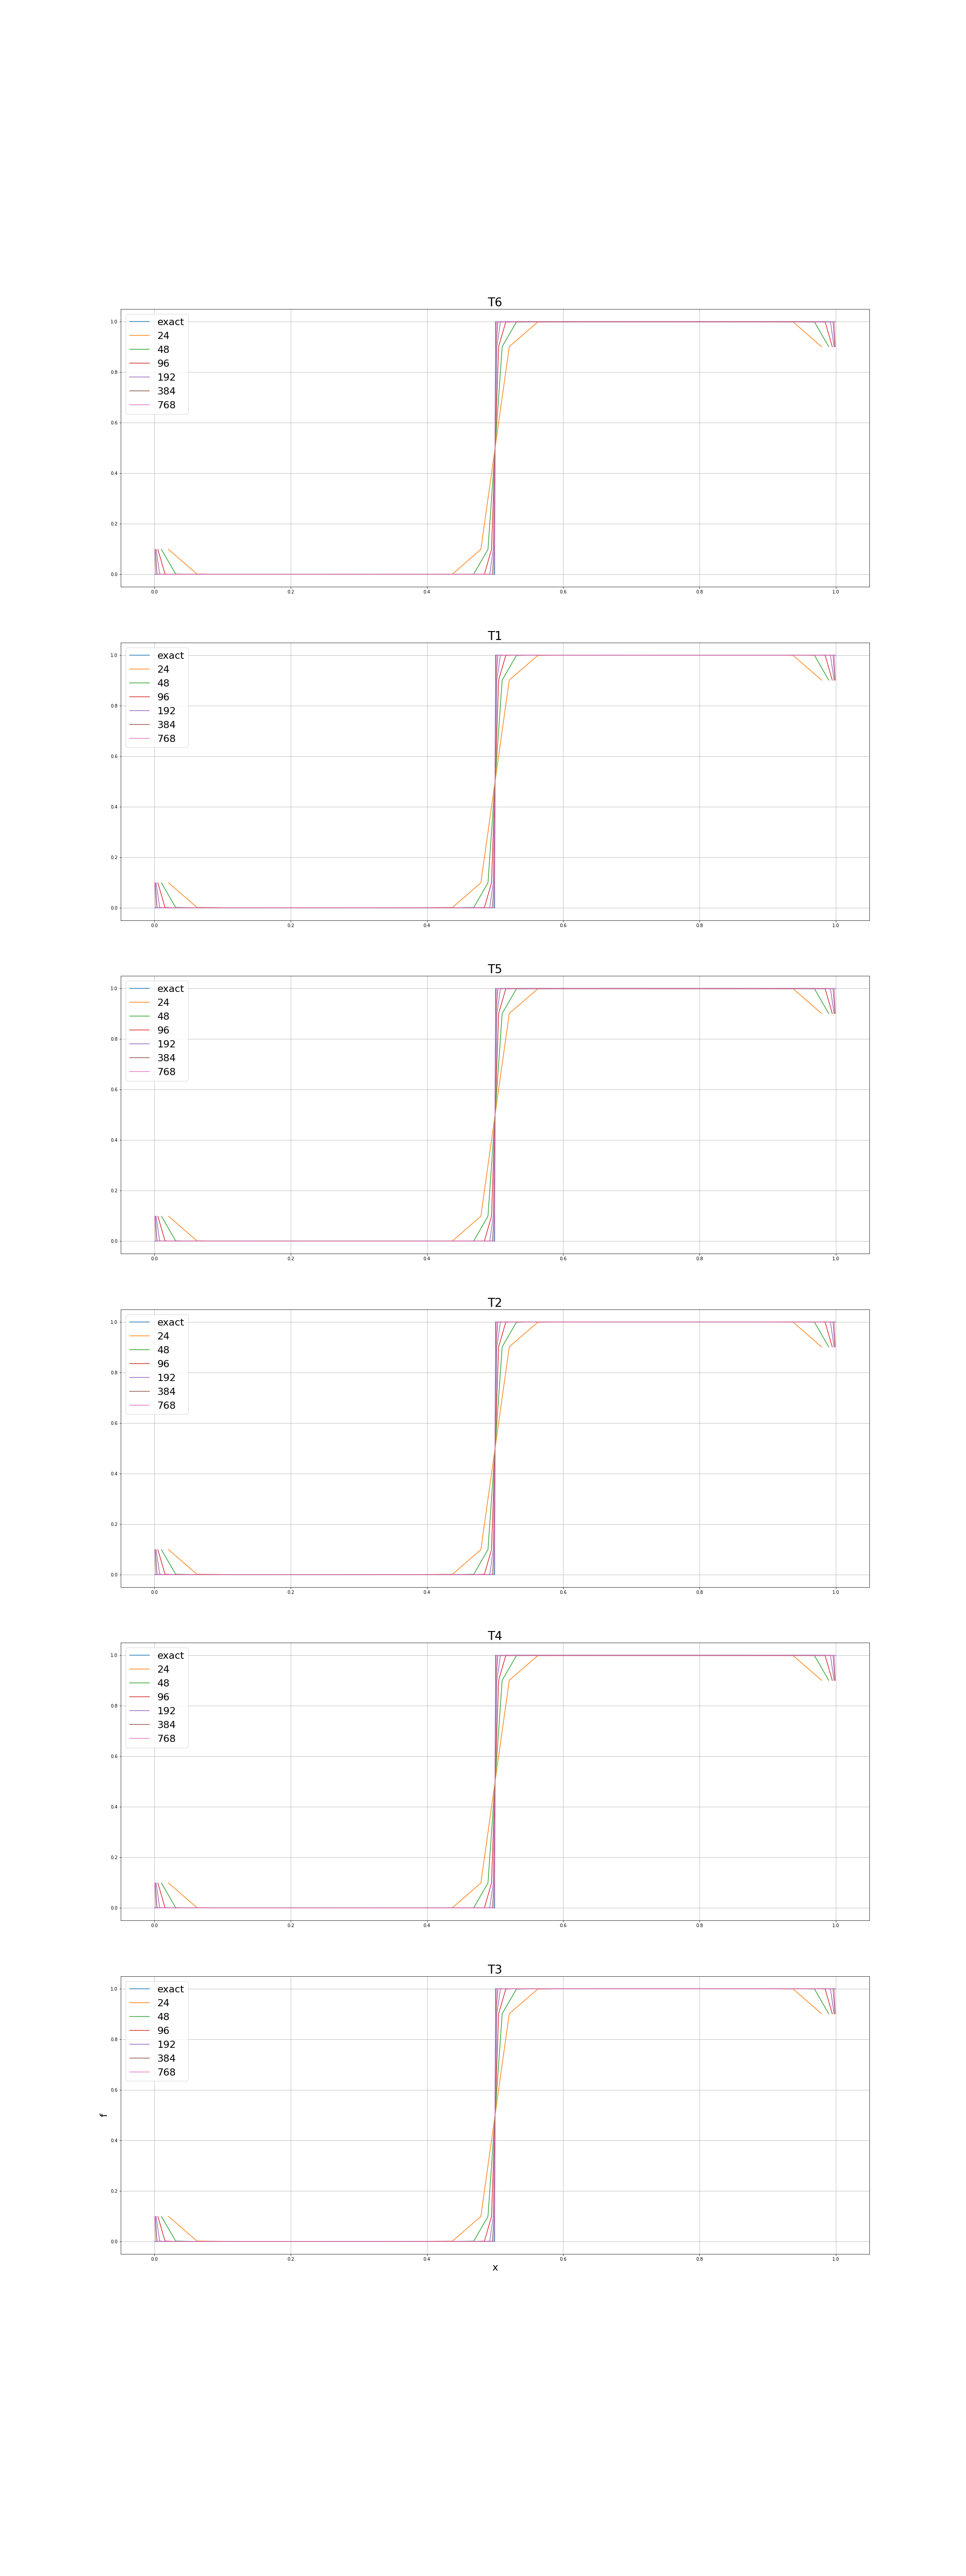
\includegraphics[width=0.5\linewidth]{Pictures/THINC_MUSCL.png}
 \captionof{figure}{Расчеты 1D. Схема THINC + MUSCL}
 \label{fig:THINC_MUSCL}
\end{minipage}
}
\medskip
\\
Можно наблюдать значительное, по сравнению с классическими методами, уменьшение "размазывание" значений характеристической функции.

\subsection{Метод JR (Jump Reconstruction)}
Метод Jump Reconstruction позволяет в точности восстановить значения характеристической функции благодаря аппроксимации скачка разрывной функцией.
\\
\makebox[0pt][l]{%
\begin{minipage}{\textwidth}
\centering
    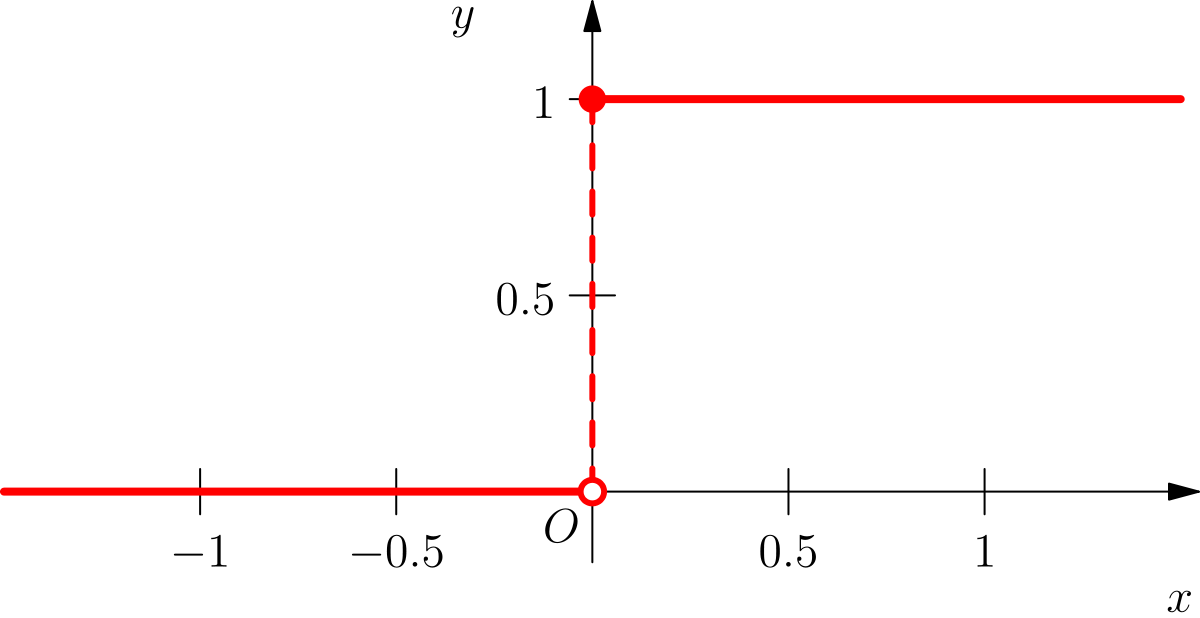
\includegraphics[width=0.5\linewidth]{Pictures/JR_func.png}
 \captionof{figure}{Разрывная функция}
 \label{fig:JR_func}
\end{minipage}
}
\medskip
\\
Интерполяционная функция $\Psi_i(x)$ строится на тех же ячейках, где выполняются условия схемы THINC:
\[
\begin{cases}
\epsilon<f_i^n<1-\epsilon & \text{то есть, }f_i^n\in(0; 1)
\\
(f_{i+1}^n-f_i^n)(f_i^n-f_{i-1}^n) & \text{условие монотонности}
\end{cases}
\]
Где $\epsilon$ - малая величина. В расчетах использовалось значение $\epsilon=1e-4$.\\
В тех ячейках, где данное условие не выполняется, используется схема Годунова или MUSCL.\\
Для аппроксимации функции  на каждом  отрезке строится функция:
\[
F_i(x)=\frac{(1-\gamma_i)}{2}+\gamma_iH(x-x_i^*)
\]
Где $H(x)$ - функция Хевисайда.\\
Параметр $x_i^*$ – положение прыжка $f$.
$x_i^*$ определяется из интегрального уравнения:
\[
f_i^n=\frac{1}{\Delta x}\int_{x_{i-\frac{1}{2}}}^{x_{i+\frac{1}{2}}}\Psi_i(x)dx
\]
Аналитическое решение данного уравнения:
\[
f_i^n=\frac{1}{\Delta x}\int_{x_{i-\frac{1}{2}}}^{x_{i+\frac{1}{2}}}(f_{min}+
\frac{(1-\gamma_i)}{2}+\gamma_iH(x-x_i^*))\Delta f_i)dx
\]
\[
x_i^*=x_{i+\frac{1}{2}} - \Delta x_i(\frac{f_{i}-f_{min}}{\Delta f_i\gamma_i}-\frac{1-\gamma_i}{2\gamma_i})
\]

Таким образом, общий алгоритм построения  на ячейке выглядит следующим образом:
\begin{enumerate}
\item По значениям $f_{i-1}^n$ и $f_{i+1}^n$ рассчитываются значения $\gamma_i$, $f_{min}$, $f_{max}$, $\Delta f_i$.
\item По значениям $gamma_i$, $f_i^n$, $f_{min}$, $\Delta f_i$ вычисляется значение $x_i^*$, необходимое для задания функции $F_i(x)$.
\item Теперь готово все необходимое для задания функции $\Psi_i(x)=f_{min}+F_i(x)\Delta f_i$ на отрезке $\Delta x_i$.
\end{enumerate}
Однако для вычисления интегралов потоков при данном методе с кусочно - постоянным восполнением необходим точный расчет интегралов, описанный в разделе (\ref{sec:JR_flows}).

Результаты расчетов с помощью комбинации схемы JR и схемы Годунова, после прохождения 1-6 периодов на разных сетках представлены ниже:
\\
\makebox[0pt][l]{%
\begin{minipage}{\textwidth}
\centering
    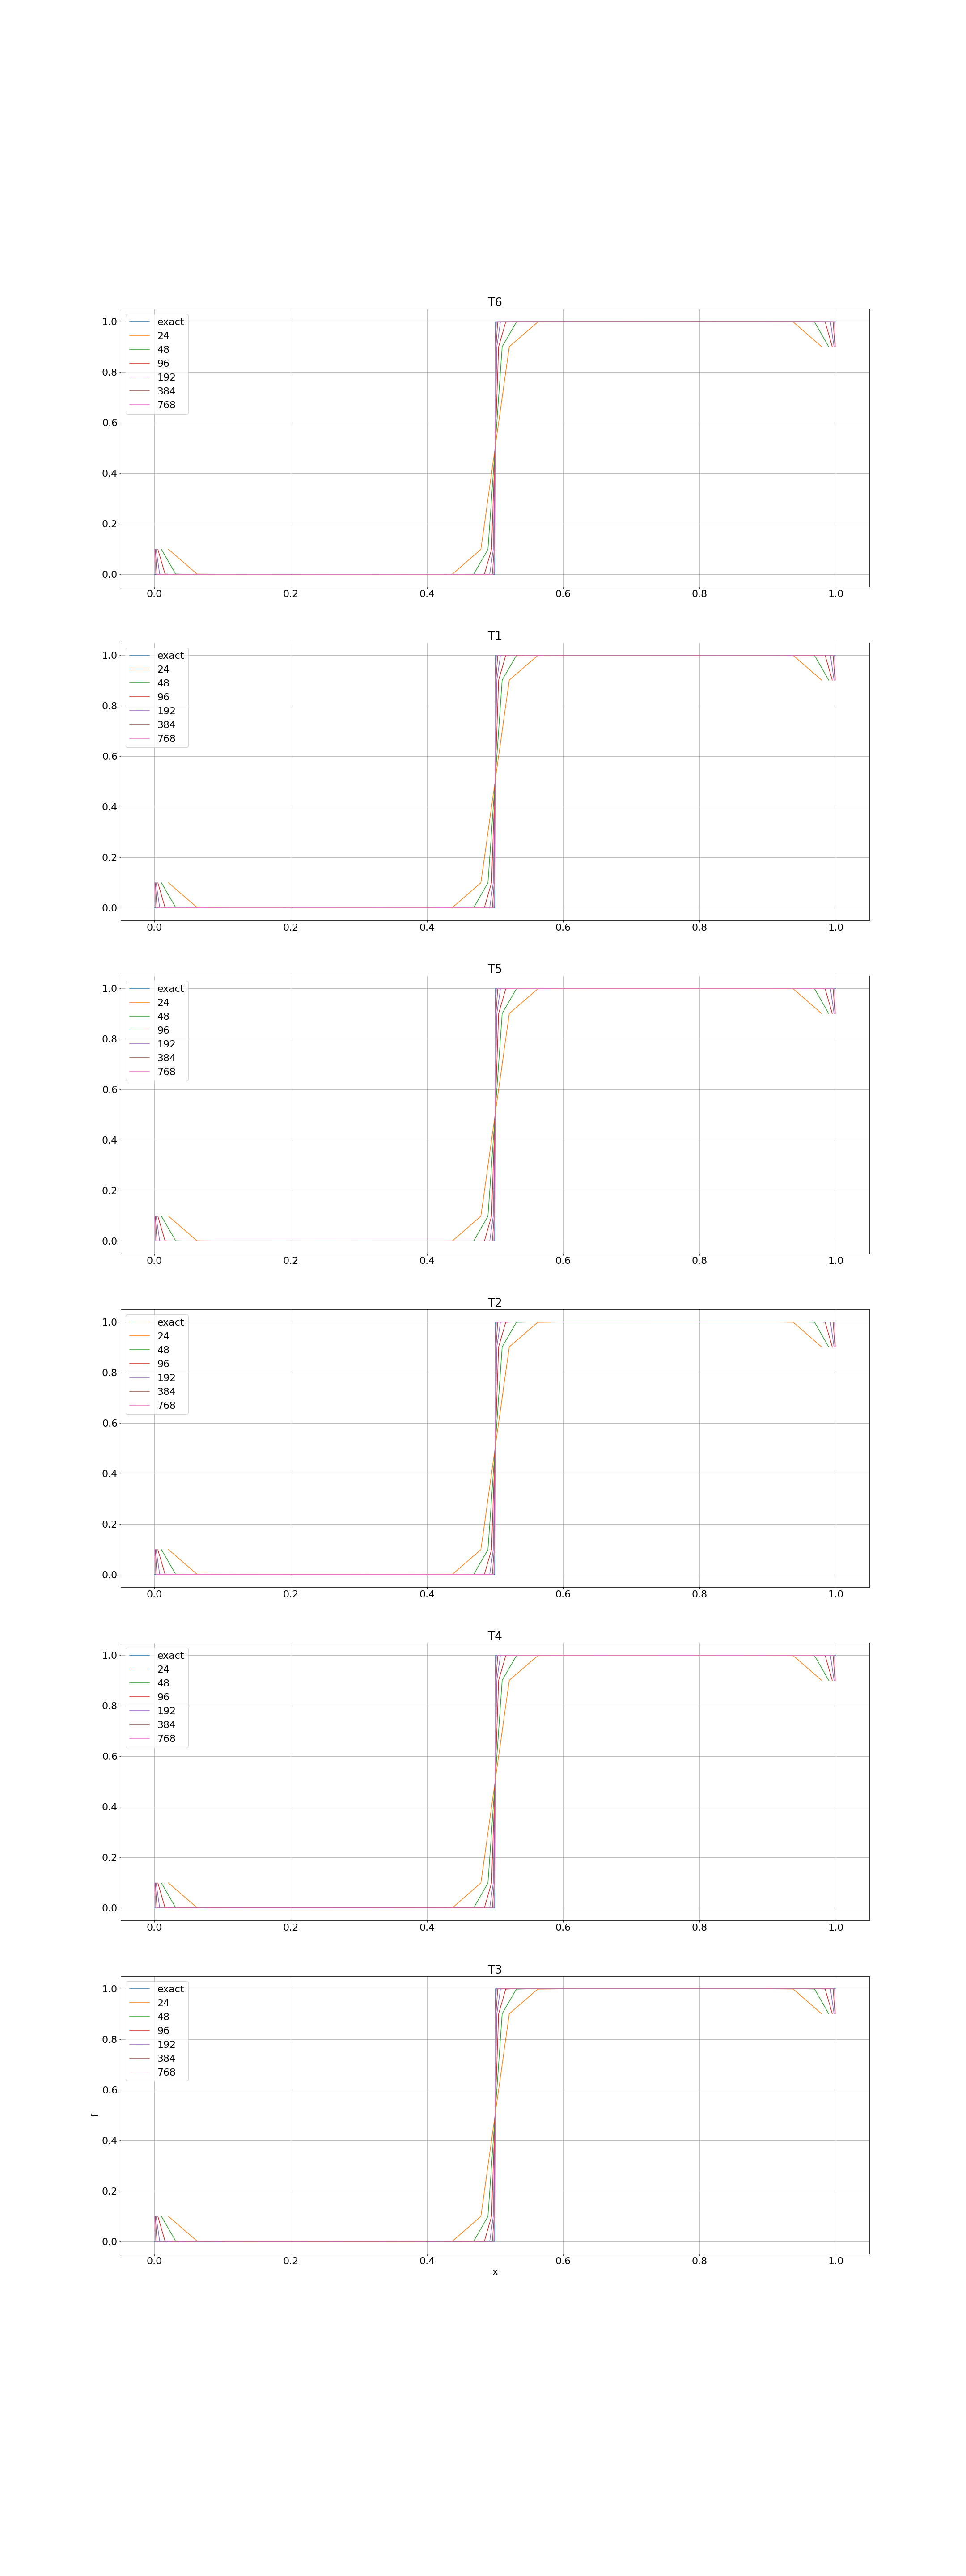
\includegraphics[width=0.5\linewidth]{Pictures/THINC_Godunov.png}
 \captionof{figure}{Расчеты 1D. Схема JR + Годунов}
 \label{fig:JR_Godunov}
\end{minipage}
}
\medskip
\\
Таким образом, при использовании метода Jump Reconstruction в одномерном случае на каждом временном шаге не происходит "размазывания" значений, и присутствует единственная ячейка с переходными значениями объемных долей. Таким образом, решение в одномерном случае получается точным. 

\subsection{Тестовые расчеты}
Таким образом, программа для расчета движения строится следующим образом:\\
Начальные условия – значения $f_i^0$, которые аппроксимирую скалярную величину $f$ заданы в массиве.
\\
\makebox[0pt][l]{%
\begin{minipage}{\textwidth}
\centering
    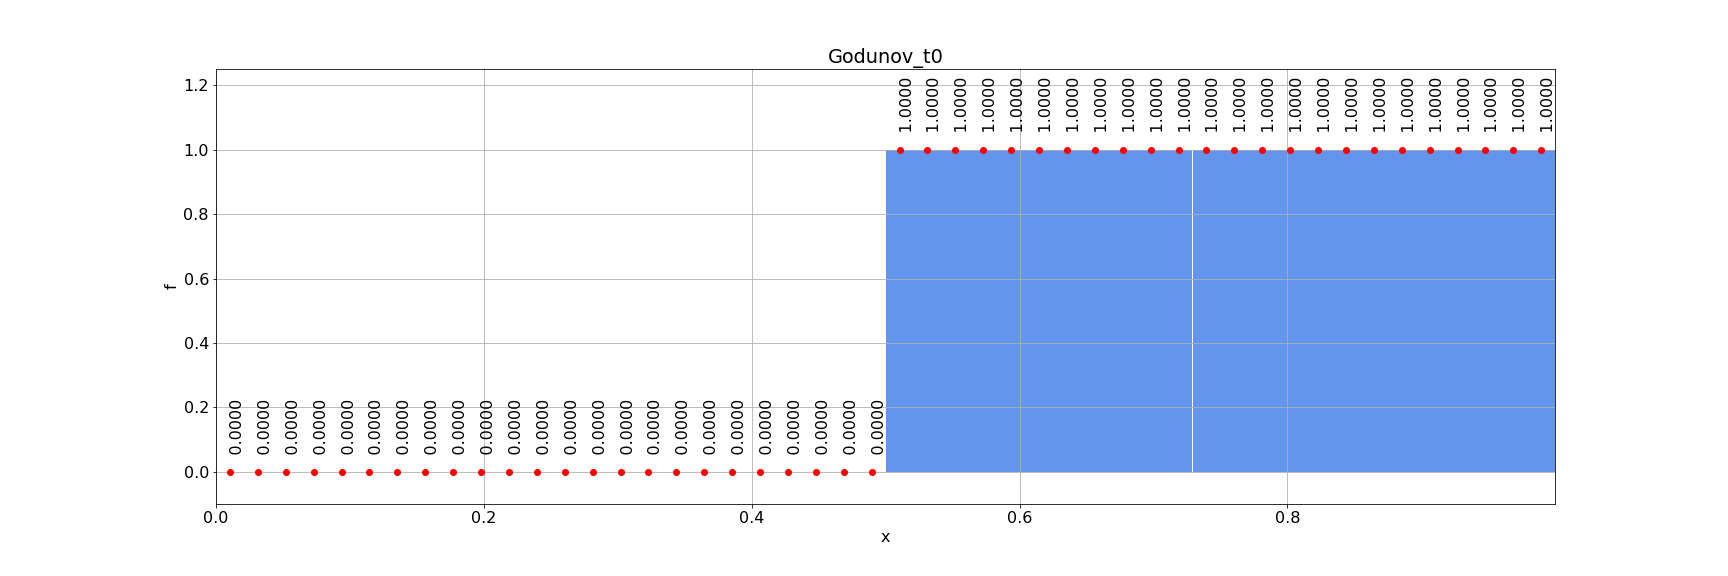
\includegraphics[width=\linewidth]{Pictures/Godunov_t0.png}
 \captionof{figure}{Начальные условия для тестовых расчетов}
\end{minipage}
}
\medskip
\\
Исследуемая область устроена таким образом, что последняя ячейка $i=cellCount-1$ - предыдущая для первой ячейки $i$, и наоборот. То есть вся область представляет собой кольцо, заданы периодические граничные условия. Количество ячеек подобрано таким образом, чтобы «планка» проходила полный круг за целое число шагов по времени. Тогда после прохождения каждого периода точное решение будет соответствовать начальным условиям.
Размер ячеек постоянен и равен соответственно:
\[
\Delta x=\frac{L}{N}
\]
Шаг по времени выбирается в соответствие с условием Куранта по формуле: 
\[
\Delta t=CFL\frac{\Delta x}{u}
\]
Тогда для прохождения одного периода потребуется T шагов по времени:
\[
T=\frac{N}{CFL}
\]
Все расчеты производились с числом CFL=0.3. Это позволило убрать нежелательные осцилляции в методе THINC при расчете рядом с границей скачка. Количество ячеек сетки N тогда было выбрано: [24, 48, 96, 192, 384, 768]. При расчетах использовалась скорость u=0.1.
На каждом шаге по времени происходит вычисление новых значений $f_i^{n+1}$ через потоки, которые рассчитываются в соответствии с выбранным методом восполнения.\\
Функция $\Psi_i(x)$ выбирается на каждой ячейке в соответствии со схемой расчетов. Для каждого следующего отрезка $\Delta x_{i+1}$ мы сохраняем функцию $\Psi_i(x)$, и используем ее в качестве $\Psi_{i-1}(x)$.\\
Таким образом, мы делаем шаг по времени для всех отрезков $\Delta x_{i}$.

Пример программной реализации на языке программирования C++ численного решения уравнения переноса в одномерном случае находится в Приложении [\ref{code:TESolver1D}].\\
Результаты расчетов были визуализированы с помощью программы на языке Python.\\
Примеры расчетов для используемых методов на сетках с разным разрешением:
\\
\makebox[0pt][l]{%
\begin{minipage}{\textwidth}
\centering
    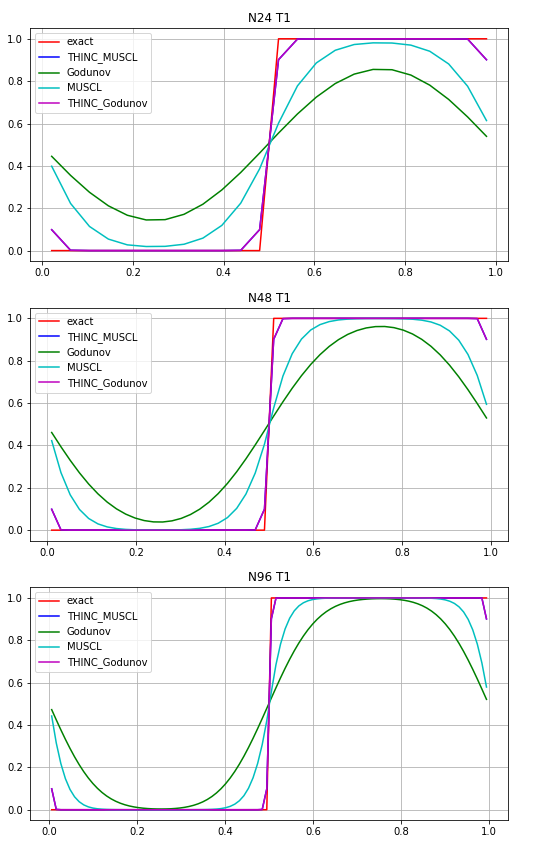
\includegraphics[width=\linewidth]{Pictures/solutions_N24_96_T1.png}
 \captionof{figure}{Расчеты 1D движения планки различными методами. Число ячеек 24, 48, 96. Прохождение 1 периода.}
\end{minipage}
}
\medskip
\\
\makebox[0pt][l]{%
\begin{minipage}{\textwidth}
\centering
    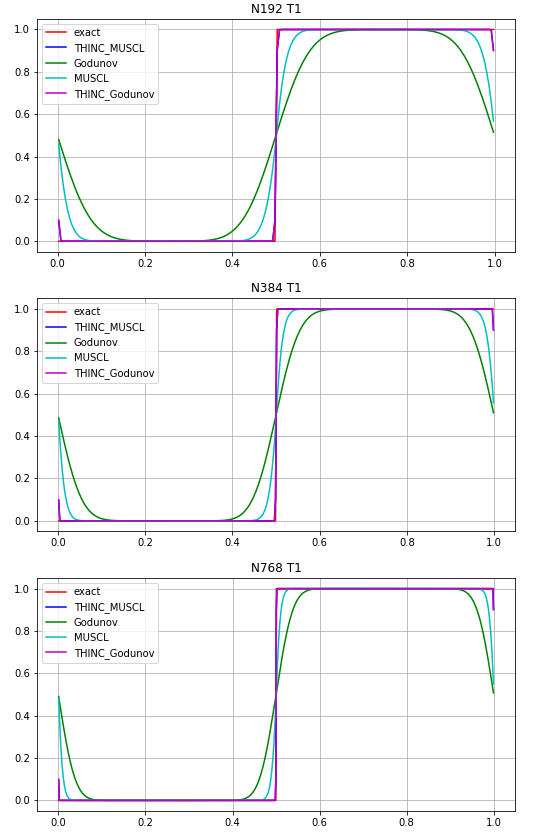
\includegraphics[width=\linewidth]{Pictures/solutions_N192_768_T1.png}
 \captionof{figure}{Расчеты 1D движения планки различными методами. Число ячеек 192, 384, 768. Прохождение 1 периода.}
\end{minipage}
}
\medskip
\\
\makebox[0pt][l]{%
\begin{minipage}{\textwidth}
\centering
    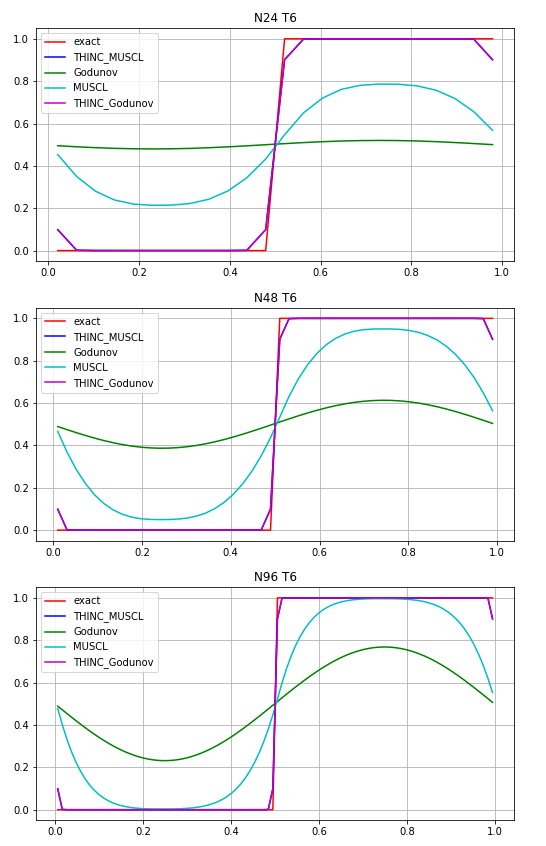
\includegraphics[width=\linewidth]{Pictures/solutions_N24_96_T6.png}
 \captionof{figure}{Расчеты 1D движения планки различными методами. Число ячеек 24, 48, 96. Прохождение 6 периодов.}
\end{minipage}
}
\medskip
\\
\makebox[0pt][l]{%
\begin{minipage}{\textwidth}
\centering
    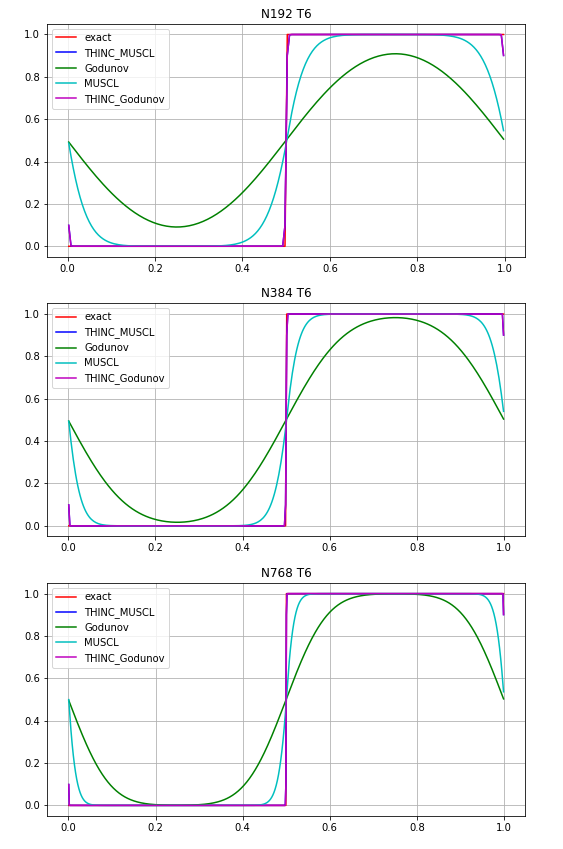
\includegraphics[width=\linewidth]{Pictures/solutions_N192_768_T6.png}
 \captionof{figure}{Расчеты 1D движения планки различными методами. Число ячеек 192, 384, 768. Прохождение 6 периодов.}
\end{minipage}
}
\medskip
\\

\subsection{Исследование сходимости}
\paragraph{Расчет ошибки}
Для всех вычислений была рассчитана ошибка по норме $l_2$ по формуле:
\[
error_{l_2}(N, T)=\sqrt{\sum_{i=0}^{N-1}((f_i^T-f_i^{exact})\Delta x)^2}
\]
Где $f_i^{exact}=f_i^0$ (так как планка проходит целое число периодов).

Данная ошибка была вычислена после прохождения T=[1..6] периодов на сетках с N=[24, 48, 96, 192, 384, 768] ячейками. Соответствующие таблицы ошибок для всех методов представлены ниже:

\begin{center}
\begin{tabular}{|c|c|c|c|c|c|c|}
\hline
  & T1 & T2 & T3 & T4 & T5 & T6 \\
\hline
N24 & 0.0595699 & 0.0768529 & 0.0876215 & 0.0938853 & 0.0974552 & 0.0994732 \\
\hline
N48 & 0.0343195 & 0.0422635 & 0.0489433 & 0.0543952 & 0.0586747 & 0.0619692 \\
\hline
N96 & 0.0203693 & 0.024306 & 0.0272539 & 0.0299097 & 0.0323704 & 0.0346239 \\
\hline
N192 & 0.0121176 & 0.0144143 & 0.015962 & 0.0171938 & 0.0182741 & 0.0192768 \\
\hline
N384 & 0.00720701 & 0.00857172 & 0.00948658 & 0.0101944 & 0.0107809 & 0.0112883 \\
\hline
N768 & 0.00428586 & 0.0050971 & 0.00564099 & 0.0060617 & 0.00640951 & 0.00670845 \\
\hline
\end{tabular}
\captionof{table}{Ошибка в схеме Годунова}
\label{tab:GodunovError}
\end{center}

\begin{center}
\begin{tabular}{|c|c|c|c|c|c|c|}
\hline
  & T1 & T2 & T3 & T4 & T5 & T6 \\
\hline
N24 & 0.0392346 & 0.0445669 & 0.0490333 & 0.0534235 & 0.0576686 & 0.0616839 \\
\hline
N48 & 0.0223648 & 0.0253282 & 0.0271637 & 0.028482 & 0.0295385 & 0.0304656 \\
\hline
N96 & 0.0126646 & 0.0143063 & 0.0153512 & 0.0161337 & 0.0167661 & 0.0173002 \\
\hline
N192 & 0.00715315 & 0.00806674 & 0.00864907 & 0.00908569 & 0.00943849 & 0.00973635 \\
\hline
N384 & 0.00403337 & 0.00454284 & 0.00486817 & 0.00511226 & 0.0053096 & 0.00547623 \\
\hline
N768 & 0.00227142 & 0.00255613 & 0.00273812 & 0.00287473 & 0.00298521 & 0.00307853 \\
\hline
\end{tabular}
\captionof{table}{Ошибка в схеме MUSCL}
\label{tab:MUSCLError}
\end{center}

\begin{center}
\begin{tabular}{|c|c|c|c|c|c|c|}
\hline
  & T1 & T2 & T3 & T4 & T5 & T6 \\
\hline
N24 & 0.00823062 & 0.00823302 & 0.00823357 & 0.00823392 & 0.00823399 & 0.00823399 \\
\hline
N48 & 0.0041157 & 0.00411636 & 0.00411636 & 0.00411657 & 0.00411685 & 0.00411681 \\
\hline
N96 & 0.00205787 & 0.00205821 & 0.00205827 & 0.00205829 & 0.00205829 & 0.00205843 \\
\hline
N192 & 0.0010291 & 0.00102914 & 0.00102914 & 0.00102922 & 0.00102921 & 0.00102922 \\
\hline
N384 & 0.000514571 & 0.000514608 & 0.000514609 & 0.000514604 & 0.000514602 & 0.000514604 \\
\hline
N768 & 0.000257304 & 0.000257302 & 0.000257302 & 0.000257301 & 0.000257302 & 0.000257302 \\
\hline
\end{tabular}
\captionof{table}{Ошибка в схеме THINC + Годунов}
\label{tab:THINC_Godunov_Error}
\end{center}

\begin{center}
\begin{tabular}{|c|c|c|c|c|c|c|}
\hline
  & T1 & T2 & T3 & T4 & T5 & T6 \\
\hline
N24 & 0.00823047 & 0.00823123 & 0.00823164 & 0.00823161 & 0.00823284 & 0.00823292 \\
\hline
N48 & 0.00411565 & 0.00411571 & 0.00411591 & 0.00411609 & 0.00411618 & 0.00411591 \\
\hline
N96 & 0.00205785 & 0.00205808 & 0.00205803 & 0.0020579 & 0.00205794 & 0.00205799 \\
\hline
N192 & 0.00102904 & 0.00102895 & 0.00102899 & 0.00102916 & 0.00102914 & 0.00102913 \\
\hline
N384 & 0.000514474 & 0.000514581 & 0.000514565 & 0.000514566 & 0.000514574 & 0.000514576 \\
\hline
N768 & 0.000257291 & 0.000257283 & 0.000257288 & 0.000257299 & 0.000257295 & 0.000257293 \\
\hline
\end{tabular}
\captionof{table}{Ошибка в схеме THINC + MUSCL}
\label{tab:THINC_MUSCL_Error}
\end{center}

Схема JR в одномерном случае дает около нулевую ошибку, так как восстанавливает решение в точности.

Из полученных данных можно сделать вывод, что использование схемы THINC дает значительное увеличение точности по сравнению с методом Годунова или MUSCL. Схема THINC позволяет на порядок уменьшить величину ошибки. Сравнивая комбинацию методов THINC + Годунов и THINC+MUSCL, можно заметить очень маленькую разницу в результатах расчетов и величинах ошибки (менее 1\%). Такой результат получается вследствие того, что вычисляемая функция $\Psi_i(x)$ в тех ячейках, где значения $f_i^n$ близки к 0 или 1 (используется MUSCL), получалась практически горизонтальной прямой, то есть самим значением $f_i^n$, как в схеме Годунова. Таким образом, нет значимой разницы в комбинировании схемы THINC со схемой Годунова или MUSCL для текущей реализации решения задачи.

\paragraph{Исследование сходимости.}
Полагая, что метод имеет порядок сходимости $\beta$, если $\exists \alpha \in (0; 1]$ такое что выполняется неравенство $error_{l_2}(N, T)\leq\alpha\Delta x^{\beta}$, было проведено исследование сходимости. Приведя неравенство к виду $ln(error_{l_2}(N, T))\leq\beta ln(\Delta x)+const$, построены графики зависимости логарифма ошибки к логарифму размера ячейки. Данные графики аппроксимируются прямыми, угол наклона которых – это порядок аппроксимации $\beta$.\\
Построенные графики с рассчитанными значениями порядка сходимости представлены ниже:
\\
\makebox[0pt][l]{%
\begin{minipage}{\textwidth}
\centering
    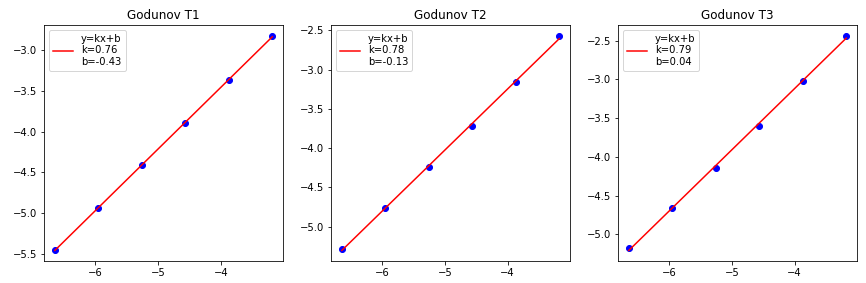
\includegraphics[width=\linewidth]{Pictures/Godunov_conv_T1_3.png}
 \captionof{figure}{Графики сходимости для схемы Годунова. Период 1-3}
\end{minipage}
}
\medskip
\\
\makebox[0pt][l]{%
\begin{minipage}{\textwidth}
\centering
    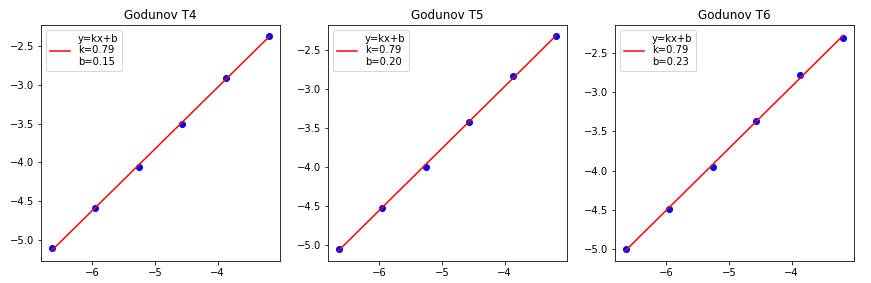
\includegraphics[width=\linewidth]{Pictures/Godunov_conv_T4_6.png}
 \captionof{figure}{Графики сходимости для схемы Годунова. Период 4-6}
\end{minipage}
}
\medskip
\\
\makebox[0pt][l]{%
\begin{minipage}{\textwidth}
\centering
    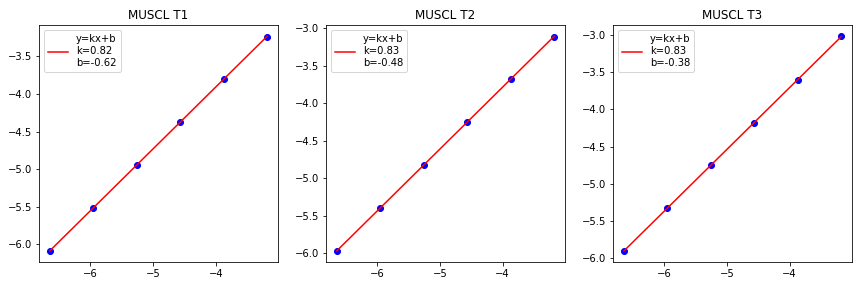
\includegraphics[width=\linewidth]{Pictures/MUSCL_conv_T1_3.png}
 \captionof{figure}{Графики сходимости для схемы MUSCL. Период 1-3}
\end{minipage}
}
\medskip
\\
\makebox[0pt][l]{%
\begin{minipage}{\textwidth}
\centering
    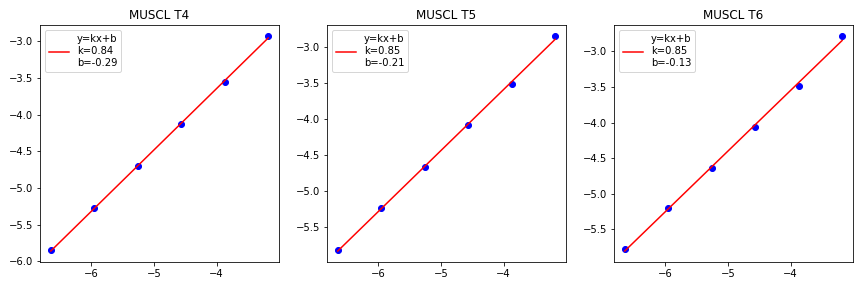
\includegraphics[width=\linewidth]{Pictures/MUSCL_conv_T4_6.png}
 \captionof{figure}{Графики сходимости для схемы MUSCL. Период 4-6}
\end{minipage}
}
\medskip
\\
\makebox[0pt][l]{%
\begin{minipage}{\textwidth}
\centering
    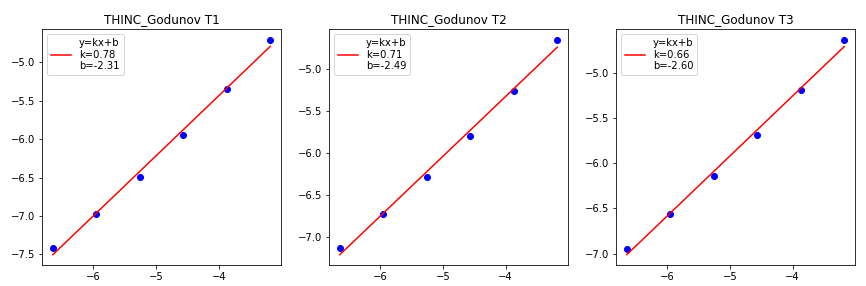
\includegraphics[width=\linewidth]{Pictures/THINC_Godunov_conv_T1_3.png}
 \captionof{figure}{Графики сходимости для схемы THINC + Годунов. Период 1-3}
\end{minipage}
}
\medskip
\\
\makebox[0pt][l]{%
\begin{minipage}{\textwidth}
\centering
    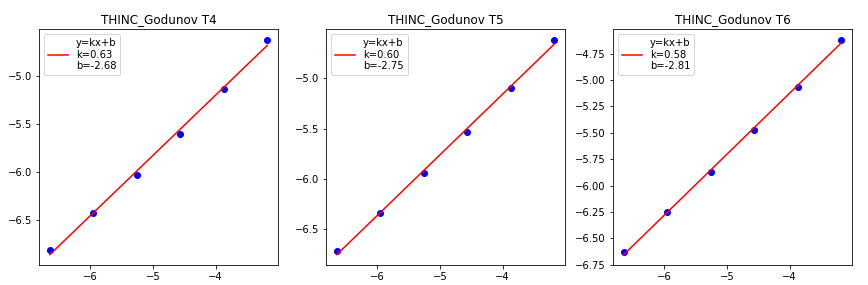
\includegraphics[width=\linewidth]{Pictures/THINC_Godunov_conv_T4_6.png}
 \captionof{figure}{Графики сходимости для схемы THINC + Годунов. Период 4-6}
\end{minipage}
}
\medskip
\\
\makebox[0pt][l]{%
\begin{minipage}{\textwidth}
\centering
    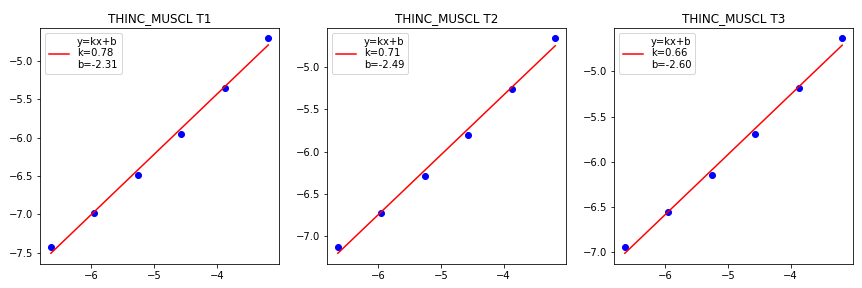
\includegraphics[width=\linewidth]{Pictures/THINC_MUSCL_conv_T1_3.png}
 \captionof{figure}{Графики сходимости для схемы THINC + MUSCL. Период 1-3}
\end{minipage}
}
\medskip
\\
\makebox[0pt][l]{%
\begin{minipage}{\textwidth}
\centering
    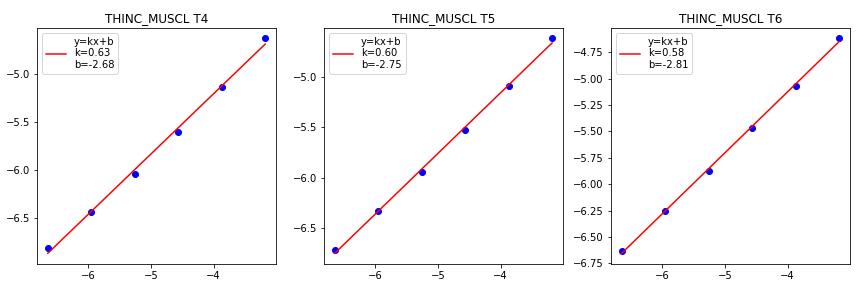
\includegraphics[width=\linewidth]{Pictures/THINC_MUSCL_conv_T4_6.png}
 \captionof{figure}{Графики сходимости для схемы THINC + MUSCL. Период 4-6}
\end{minipage}
}
\medskip
\\

\section{Многомерное обобщение решения уравнения переноса с нестационарным полем скоростей}
Алгоритм численного решения уравнения переноса для случая двух или трех измерений может быть построен на основе численного решения уравнения переноса в одномерном случае.
Исходя из вида данного уравнения в частных производных, есть возможность рассчитать решение в проекции на одном из направлений, при заданном положении данной проекции по другим направлениям.

Уравнение переноса в общем случае имеет вид (\ref{eqn:TE}):
\begin{equation}
\frac{\partial f}{\partial t}+\nabla\cdot(f\overrightarrow{u})=0
\end{equation}
В разделе (\ref{sec:TESolutionUnonstat}) проводится численное решение данного уравнения в одномерном случае (\ref{fiNextFlows}) в проекции на одну из осей. Получена алгебраическая формула для нахождения значения скалярной величины на следующем временном шаге через потоки на гранях ячеек.
\begin{equation}
f_i^{n+1}=f_i^n
-
\frac{1}{\Delta x} (
\Phi_{i+\frac{1}{2}}
-
\Phi_{i-\frac{1}{2}}
)=0
\end{equation}
Данное уравнение можно записать для каждого из направлений X,Y,Z на введенной сетке при фиксированном положении на других осях:
\begin{equation}
f_i^{n+1}=f_i^n
-
\frac{1}{\Delta x} (
\Phi_{i+\frac{1}{2}}
-
\Phi_{i-\frac{1}{2}}
)=0
\end{equation}, $i=1..N$, $j,k=const$
\begin{equation}
f_j^{n+1}=f_j^n
-
\frac{1}{\Delta x} (
\Phi_{j+\frac{1}{2}}
-
\Phi_{j-\frac{1}{2}}
)=0
\end{equation}, $j=1..M$, $i,k=const$
\begin{equation}
f_k^{n+1}=f_k^n
-
\frac{1}{\Delta x} (
\Phi_{k+\frac{1}{2}}
-
\Phi_{k-\frac{1}{2}}
)=0
\end{equation}, $k=1..P$, $i,j=const$
Скорость $u$, содержащаяся в вычислении потоков $\Phi$ постоянна на всех ячейках каждого из направлений при фиксированном положении на других направлениях, поэтому может быть использована аналогично одномерному случаю для каждого из направлений. Эта особенность характерна для поля скоростей твердого тела и описана в разделе (\ref{sec:RBVF}).

\subsection{Расщепление по направлениям}
Метод расщепления по направлениям заключается в том, что исходная задача решается в проекции на одно из направлений на сетке при фиксированных положениях данного направления по другим осям сетки. Затем полученное решение используется в качестве начальных условий для расчета по следующему направлению. В результате, для каждой ячейки сетки будут учитываться потоки на всех ее гранях.

То есть, в двумерном случае, скалярная величина, содержащаяся в каждая ячейке, представляющей собой квадрат, будет пересчитываться 2 раза. Сначала рассчитываются потоки на первой паре противоположных граней, затем, поверх изменений после прохождения по одному из направлений, на второй паре противоположных граней. При этом необходимо рассчитать M x N ячеек. То есть одномерный модуль численного алгоритма решения будет запущен M раз для каждого направления X (при каждом фиксированном значении по направлению Y) и N раз для каждого направления Y (при каждом фиксированном значении по направлению X).
Данный алгоритм может быть записан в виде:
\begin{enumerate}
\item {Решение одномерного уравнения переноса на шаге по времени $\Delta t_{n+1}$ по X направлению M раз (при Y = 1..M) при начальных условиях $f^{n}$.}
\item {Полученное решение $f'^{n+1}$ является начальными условиями для решения по направлению Y.}
\item {Решение одномерного уравнения переноса на шаге по времени $\Delta t_{n+1}$ по Y направлению N раз (при X = 1..N) при начальных условиях $f'^{n+1}$.}
\item {Полученное решение является решением для шага $\Delta t_{n+1}$: $f''^{n+1}=f^{n+1}$ и используется в качестве начальных условий для следующего шага по времени.}
\end{enumerate}

Таким образом, была реализована программа решения уравнения переноса в многомерном случае на основе модуля расчета уравнения переноса в одномерном случае. Основой данного алгоритма является расщепление по направлениям, при этом используется одномерный модуль программы, описанный в разделе (\ref{sec:TESolutionUnonstat}).

\subsection{Тестовые расчеты}
В качестве тестовых вычислений был проведен расчет движения твердого тела в поле стационарной и нестационарной скорости с элементами поступательного и вращательного движения.

Начальные условия для движения тела в поле стационарной скорости:
\[
\overrightarrow{u}(t)=(0.1, 0.1)
\]
$CFL=0.3$\\
$areaWidth=1.0$\\
$areaHeight=1.0$\\
$cellCountX=128$\\
$cellCountY=128$\\
$NTimeSteps=400$\\

Результаты расчетов для схемы Годунова:

\begin{figure}[H]
\centering
\begin{minipage}{.3\textwidth}
  \centering
  \includegraphics[width=\linewidth]{Pictures/Solve2DWhiteBearMovementTestGodunov/Solve2DWhiteBearMovementTest_t0.png}
  \captionof{figure}{t=0}
\end{minipage}%
\begin{minipage}{.3\textwidth}
  \centering
  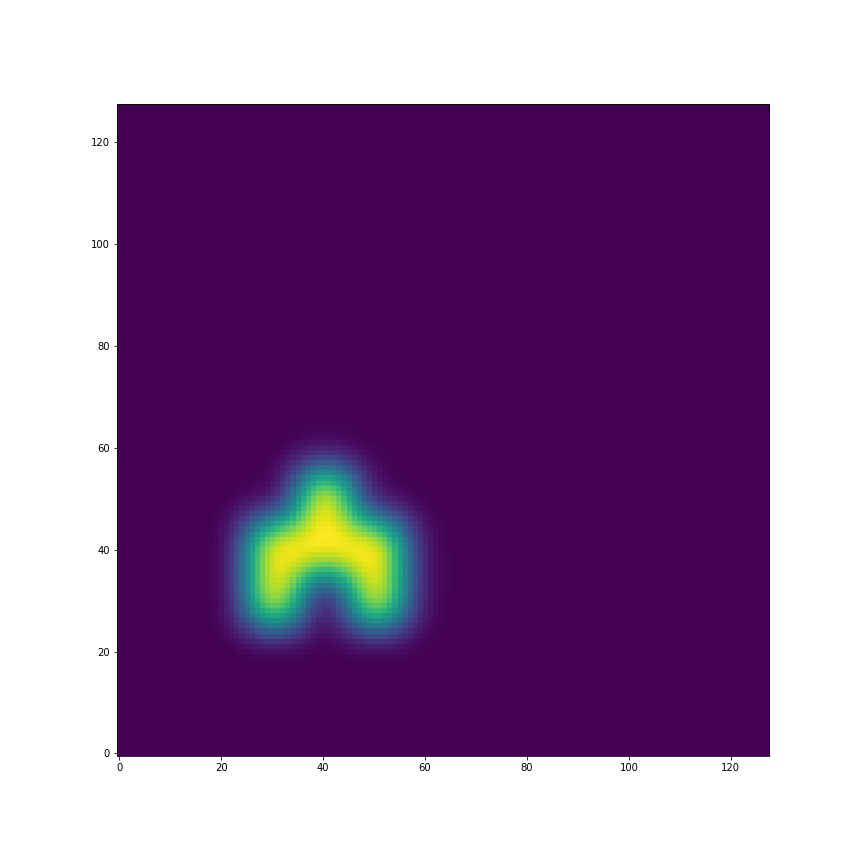
\includegraphics[width=\linewidth]{Pictures/Solve2DWhiteBearMovementTestGodunov/Solve2DWhiteBearMovementTest_t10.png}
  \captionof{figure}{t=80}
\end{minipage}%
\begin{minipage}{.3\textwidth}
  \centering
  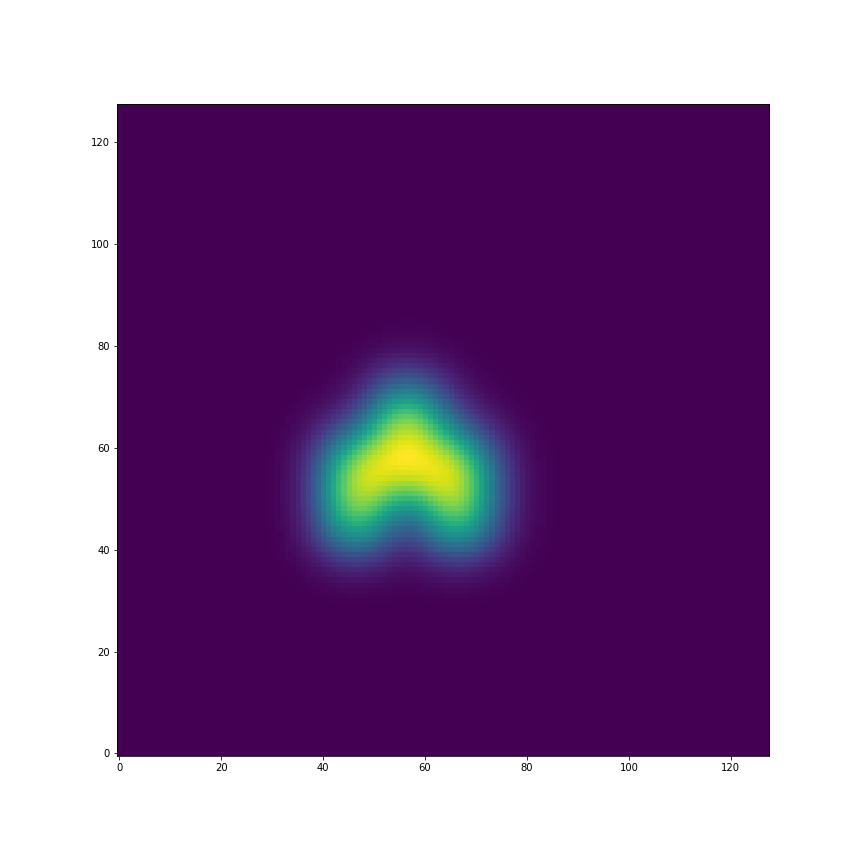
\includegraphics[width=\linewidth]{Pictures/Solve2DWhiteBearMovementTestGodunov/Solve2DWhiteBearMovementTest_t20.png}
  \captionof{figure}{t=160}
\end{minipage}
\end{figure}

\begin{figure}[H]
\centering
\begin{minipage}{.3\textwidth}
  \centering
  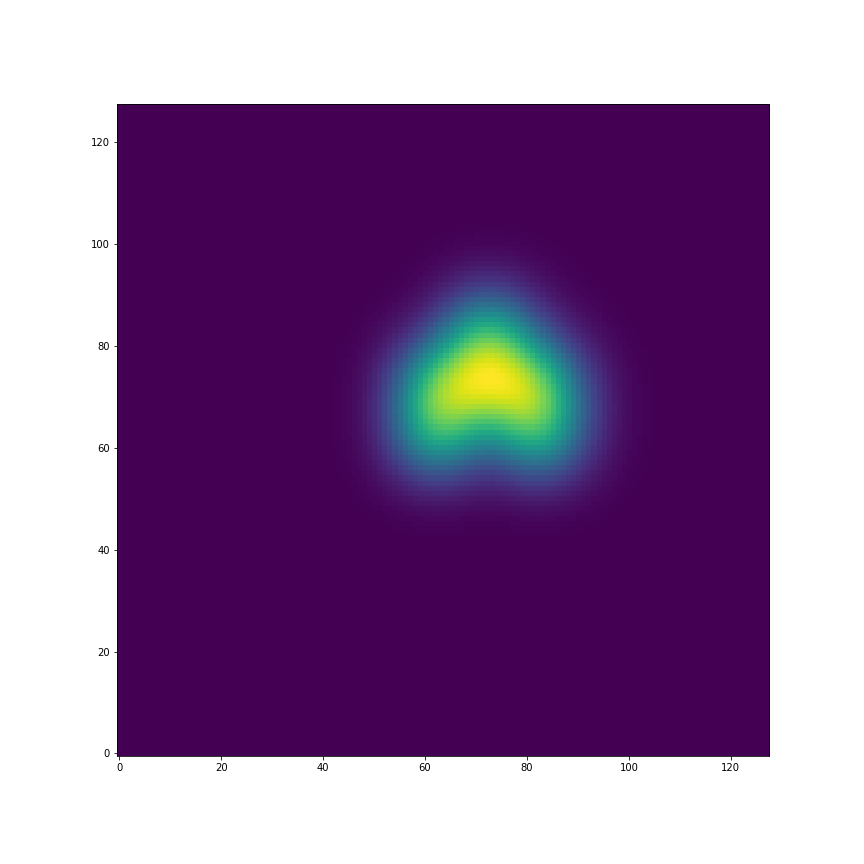
\includegraphics[width=\linewidth]{Pictures/Solve2DWhiteBearMovementTestGodunov/Solve2DWhiteBearMovementTest_t30.png}
  \captionof{figure}{t=240}
\end{minipage}%
\begin{minipage}{.3\textwidth}
  \centering
  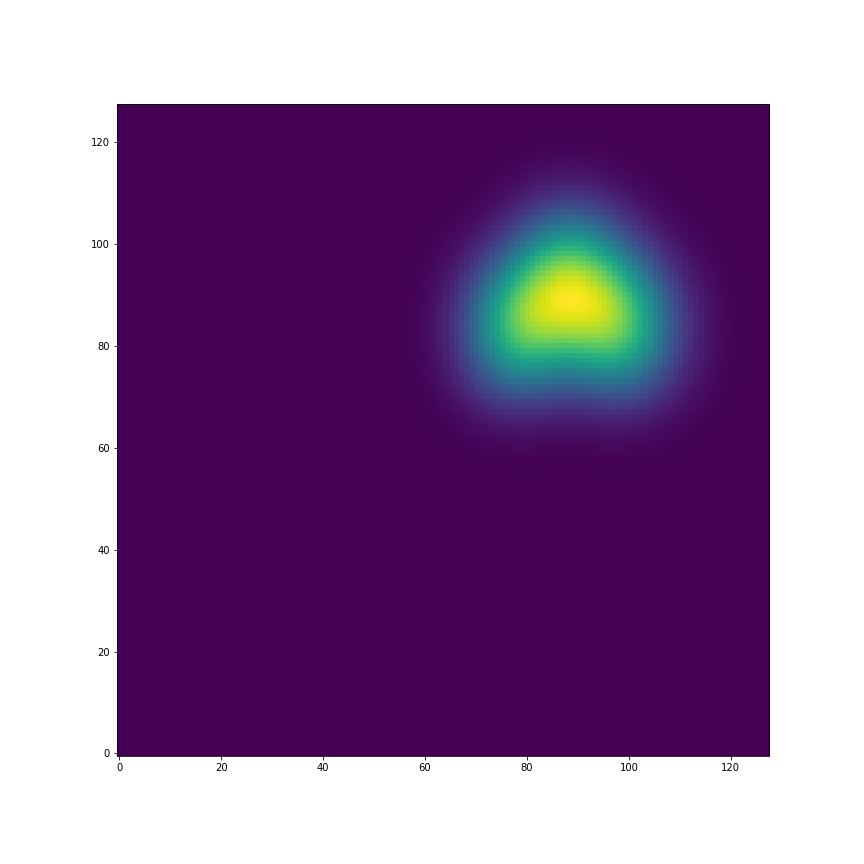
\includegraphics[width=\linewidth]{Pictures/Solve2DWhiteBearMovementTestGodunov/Solve2DWhiteBearMovementTest_t40.png}
  \captionof{figure}{t=320}
\end{minipage}%
\begin{minipage}{.3\textwidth}
  \centering
  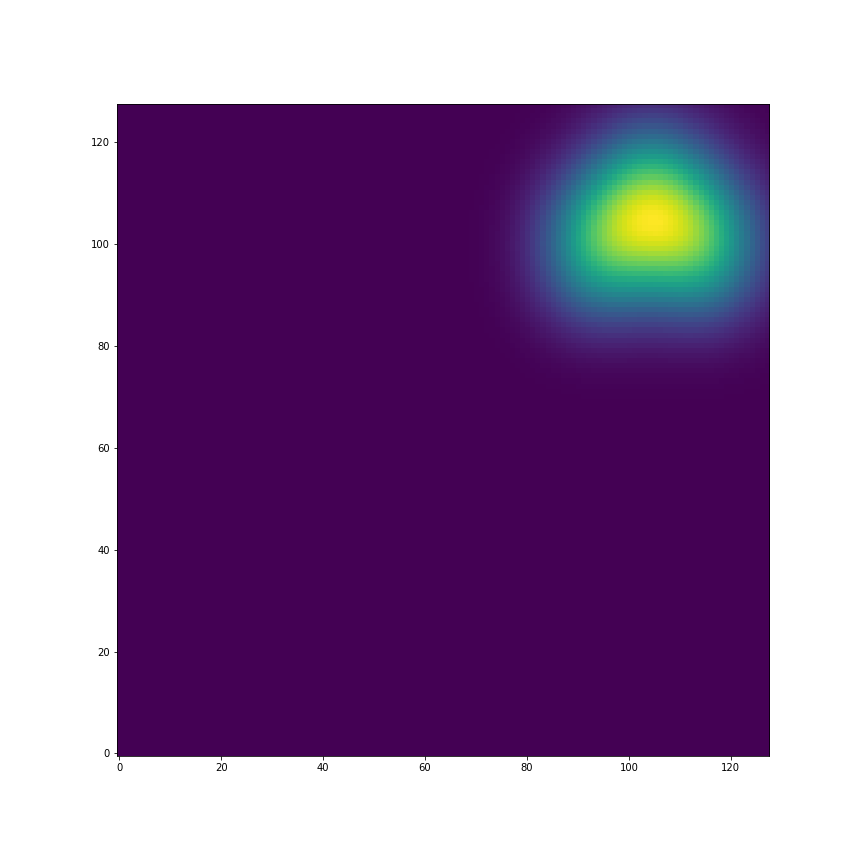
\includegraphics[width=\linewidth]{Pictures/Solve2DWhiteBearMovementTestGodunov/Solve2DWhiteBearMovementTest_t50.png}
  \captionof{figure}{t=400}
\end{minipage}
\end{figure}

Результаты расчетов для схемы MUSCL:

\begin{figure}[H]
\centering
\begin{minipage}{.3\textwidth}
  \centering
  \includegraphics[width=\linewidth]{Pictures/Solve2DWhiteBearMovementTestMUSCL/Solve2DWhiteBearMovementTest_t0.png}
  \captionof{figure}{t=0}
\end{minipage}%
\begin{minipage}{.3\textwidth}
  \centering
  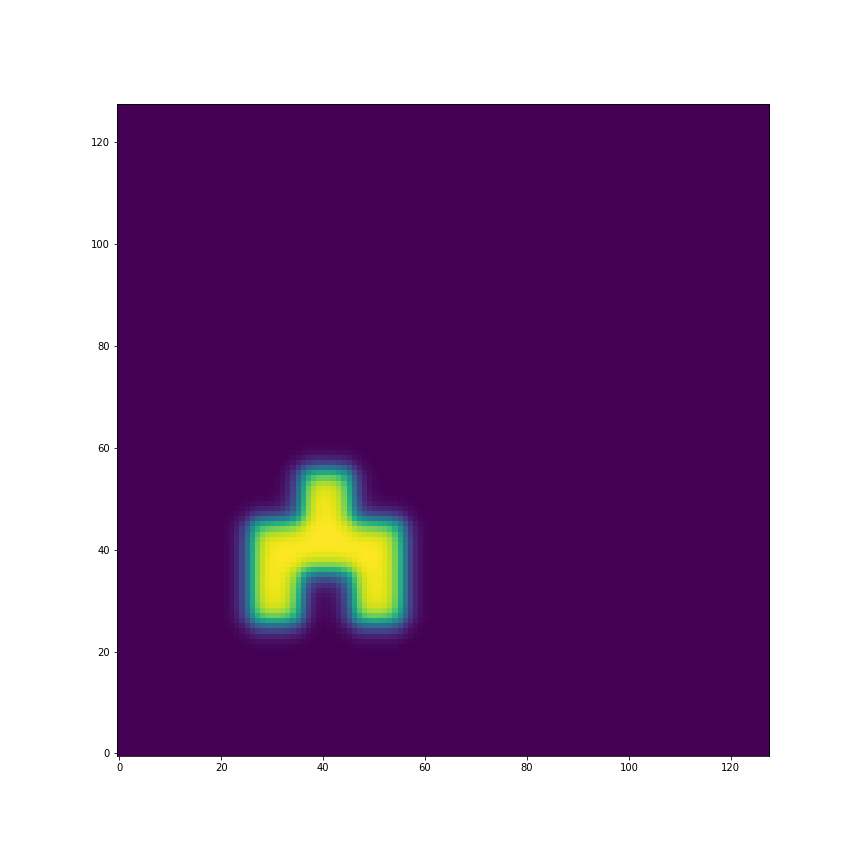
\includegraphics[width=\linewidth]{Pictures/Solve2DWhiteBearMovementTestMUSCL/Solve2DWhiteBearMovementTest_t10.png}
  \captionof{figure}{t=80}
\end{minipage}%
\begin{minipage}{.3\textwidth}
  \centering
  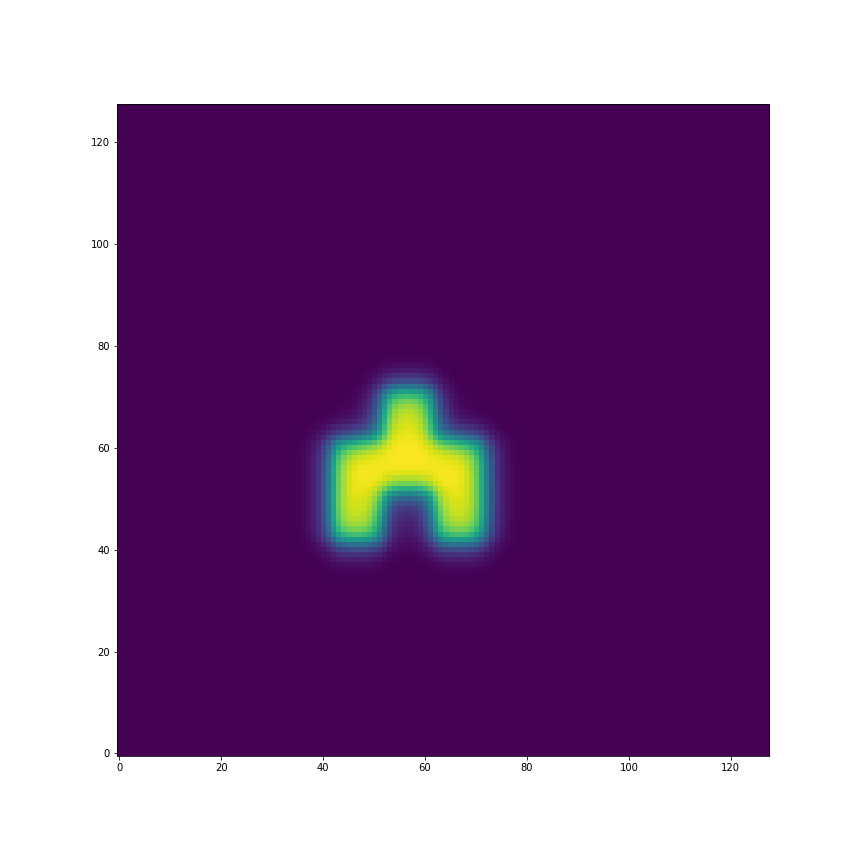
\includegraphics[width=\linewidth]{Pictures/Solve2DWhiteBearMovementTestMUSCL/Solve2DWhiteBearMovementTest_t20.png}
  \captionof{figure}{t=160}
\end{minipage}
\end{figure}

\begin{figure}[H]
\centering
\begin{minipage}{.3\textwidth}
  \centering
  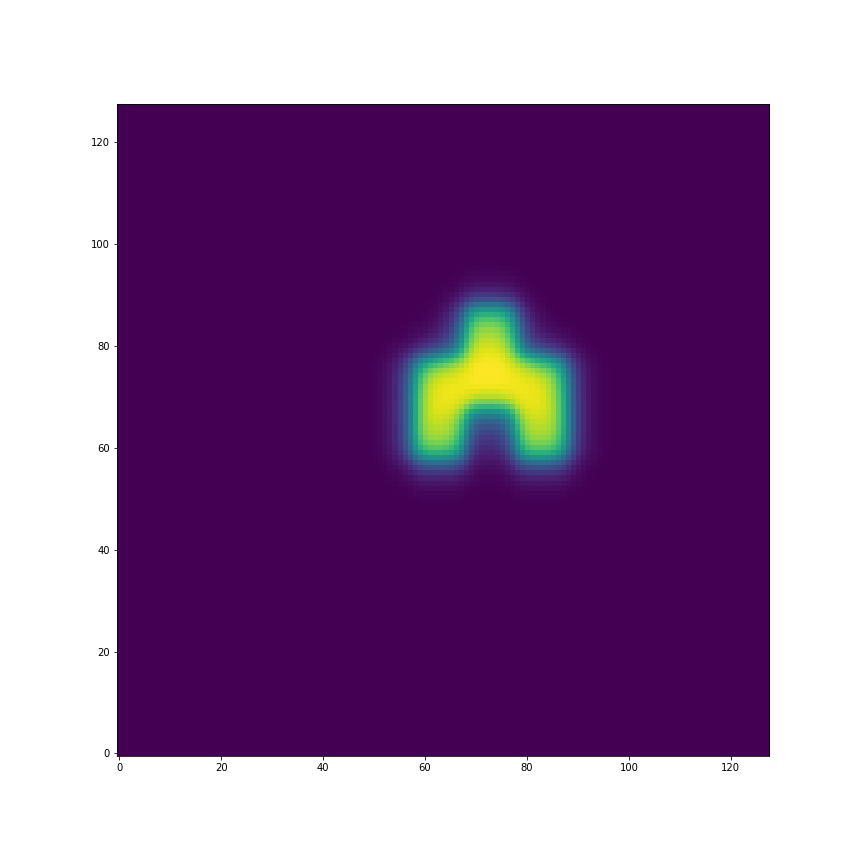
\includegraphics[width=\linewidth]{Pictures/Solve2DWhiteBearMovementTestMUSCL/Solve2DWhiteBearMovementTest_t30.png}
  \captionof{figure}{t=240}
\end{minipage}%
\begin{minipage}{.3\textwidth}
  \centering
  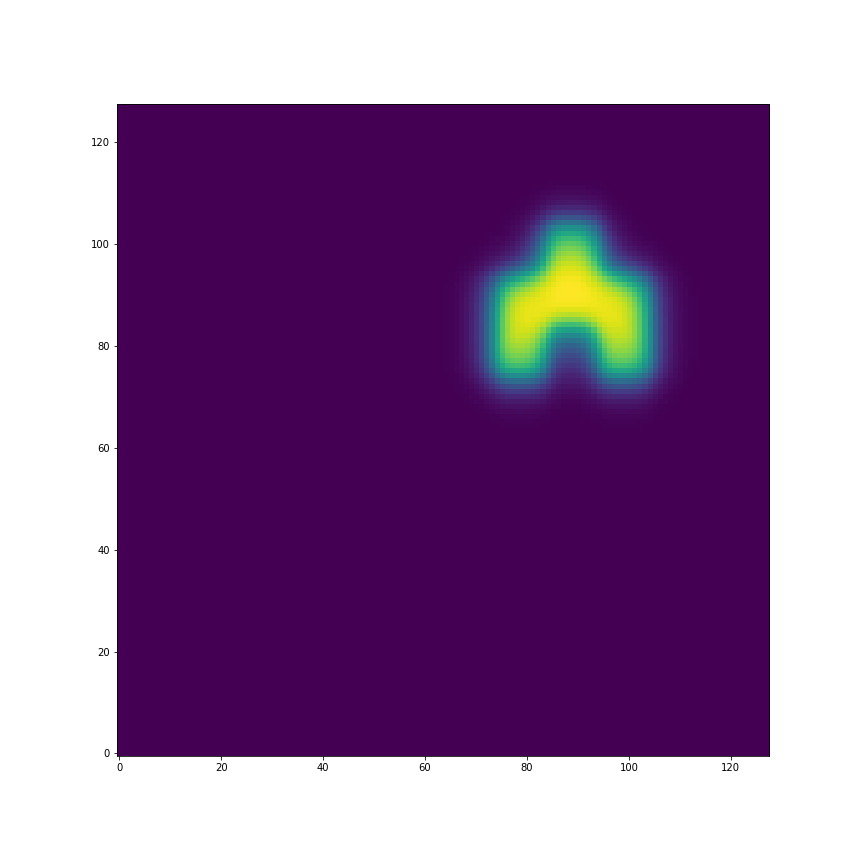
\includegraphics[width=\linewidth]{Pictures/Solve2DWhiteBearMovementTestMUSCL/Solve2DWhiteBearMovementTest_t40.png}
  \captionof{figure}{t=320}
\end{minipage}%
\begin{minipage}{.3\textwidth}
  \centering
  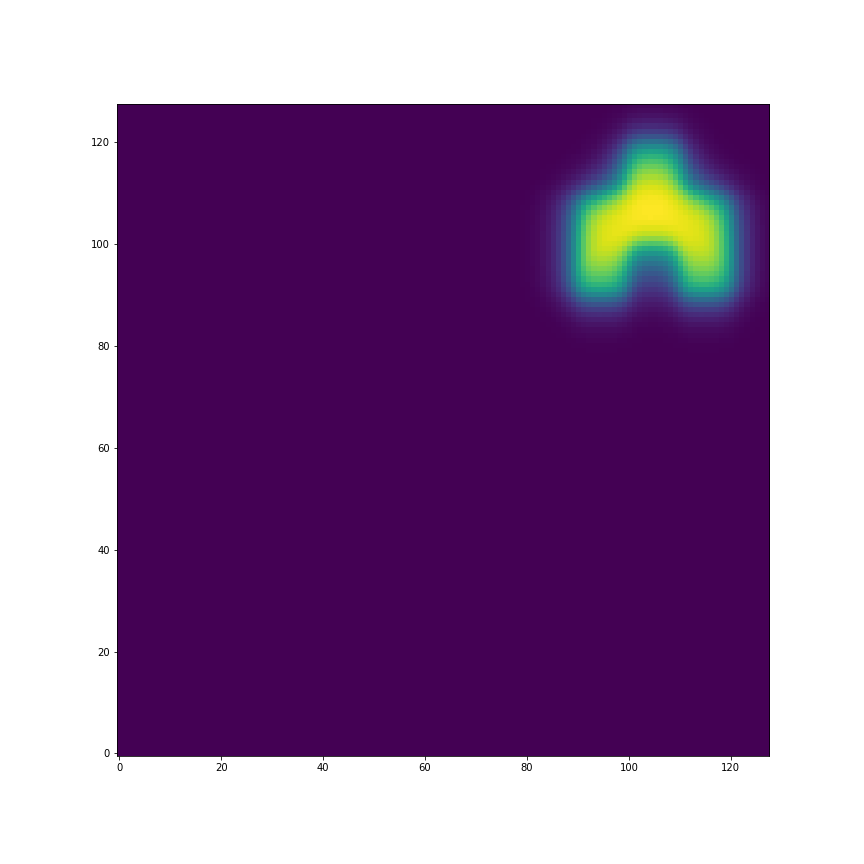
\includegraphics[width=\linewidth]{Pictures/Solve2DWhiteBearMovementTestMUSCL/Solve2DWhiteBearMovementTest_t50.png}
  \captionof{figure}{t=400}
\end{minipage}
\end{figure}

Результаты расчетов для схемы THINC:

\begin{figure}[H]
\centering
\begin{minipage}{.3\textwidth}
  \centering
  \includegraphics[width=\linewidth]{Pictures/Solve2DWhiteBearMovementTestTHINC/Solve2DWhiteBearMovementTest_t0.png}
  \captionof{figure}{t=0}
\end{minipage}%
\begin{minipage}{.3\textwidth}
  \centering
  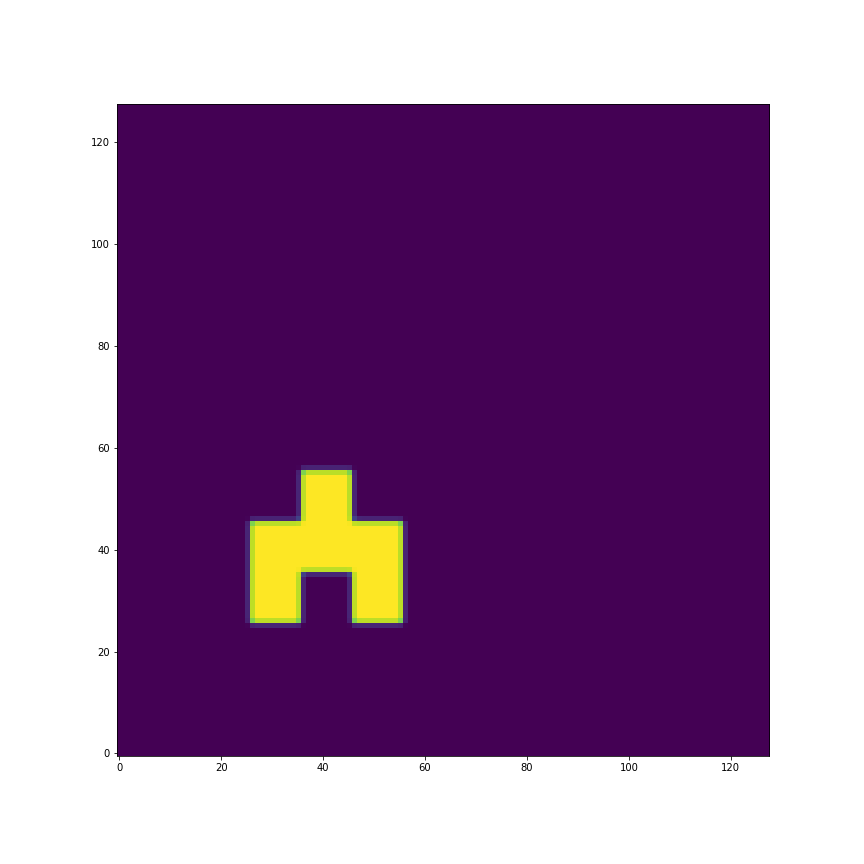
\includegraphics[width=\linewidth]{Pictures/Solve2DWhiteBearMovementTestTHINC/Solve2DWhiteBearMovementTest_t10.png}
  \captionof{figure}{t=80}
\end{minipage}%
\begin{minipage}{.3\textwidth}
  \centering
  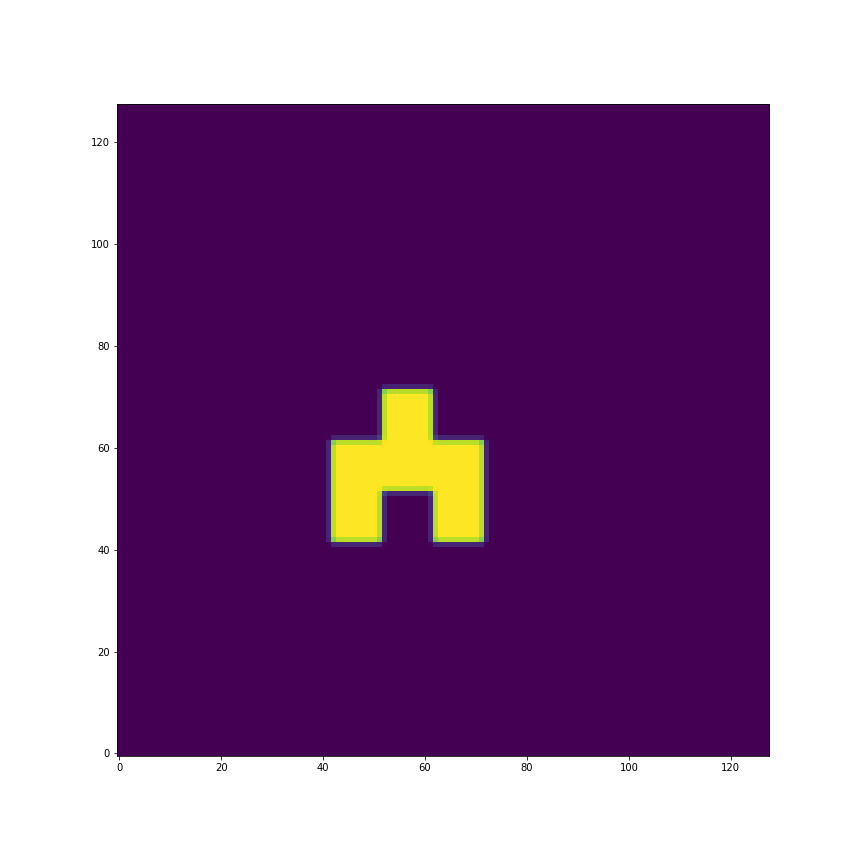
\includegraphics[width=\linewidth]{Pictures/Solve2DWhiteBearMovementTestTHINC/Solve2DWhiteBearMovementTest_t20.png}
  \captionof{figure}{t=160}
\end{minipage}
\end{figure}

\begin{figure}[H]
\centering
\begin{minipage}{.3\textwidth}
  \centering
  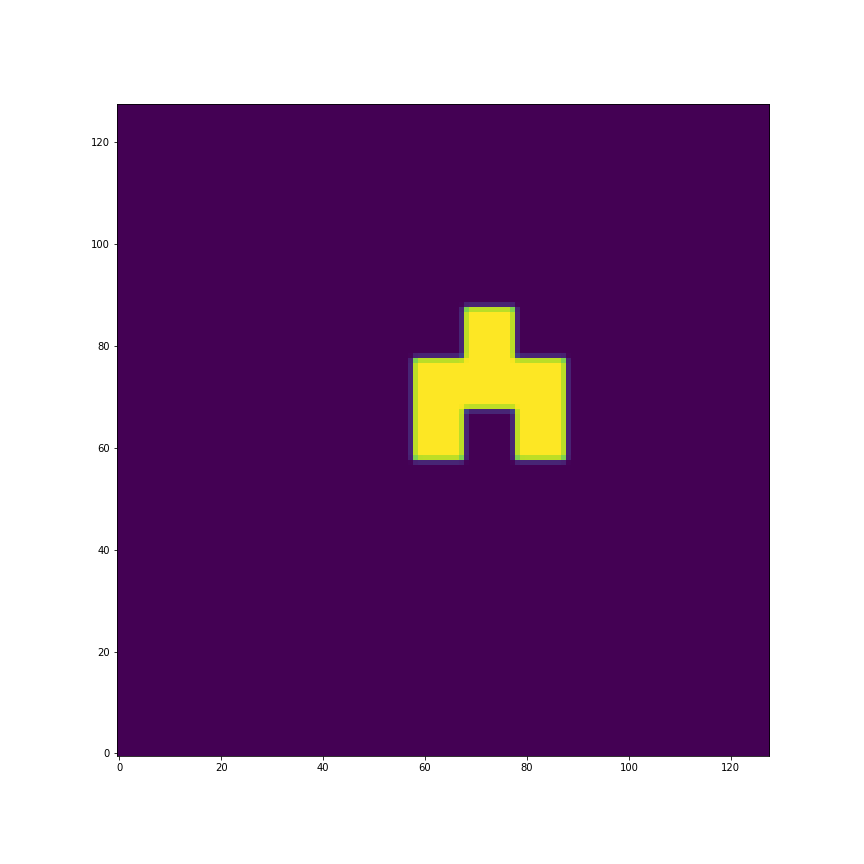
\includegraphics[width=\linewidth]{Pictures/Solve2DWhiteBearMovementTestTHINC/Solve2DWhiteBearMovementTest_t30.png}
  \captionof{figure}{t=240}
\end{minipage}%
\begin{minipage}{.3\textwidth}
  \centering
  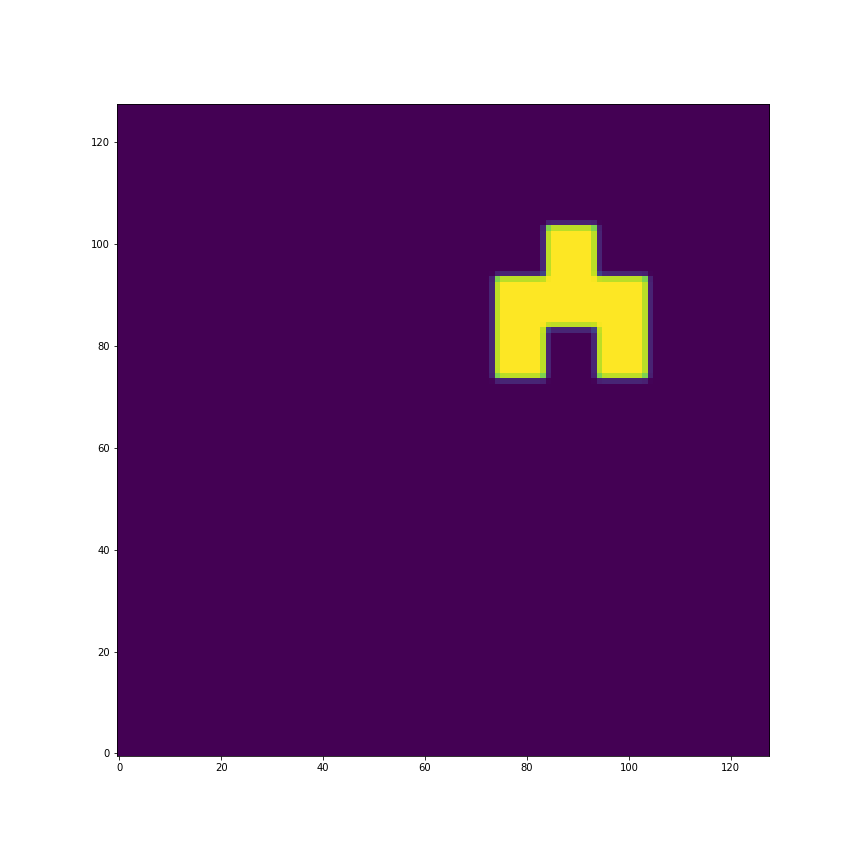
\includegraphics[width=\linewidth]{Pictures/Solve2DWhiteBearMovementTestTHINC/Solve2DWhiteBearMovementTest_t40.png}
  \captionof{figure}{t=320}
\end{minipage}%
\begin{minipage}{.3\textwidth}
  \centering
  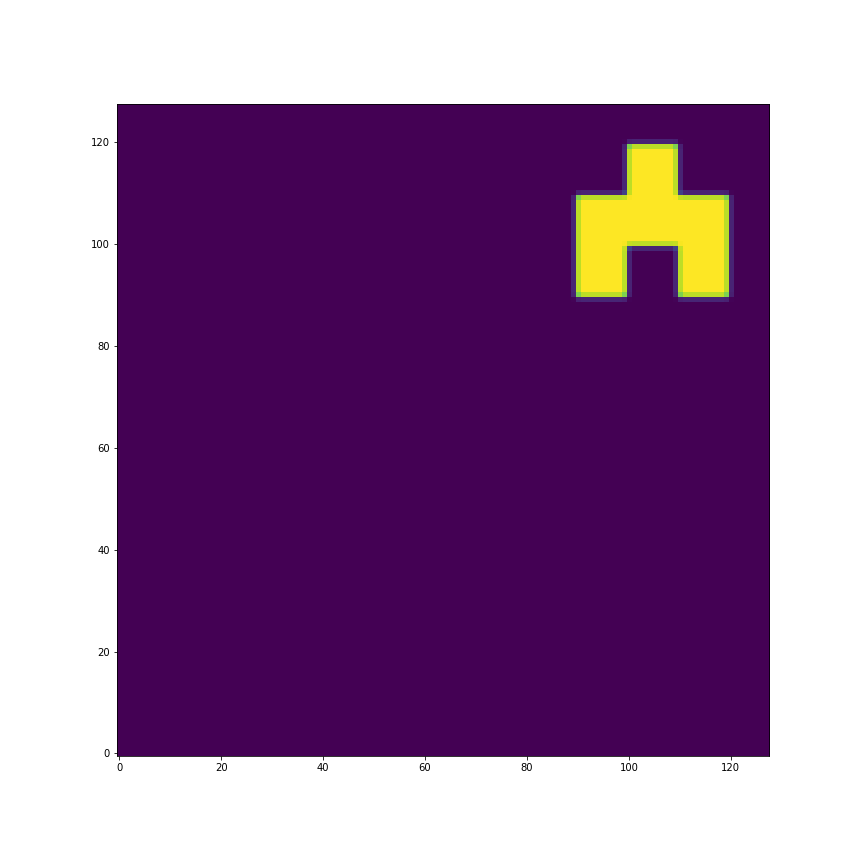
\includegraphics[width=\linewidth]{Pictures/Solve2DWhiteBearMovementTestTHINC/Solve2DWhiteBearMovementTest_t50.png}
  \captionof{figure}{t=400}
\end{minipage}
\end{figure}

Результаты расчетов для схемы JR:

\begin{figure}[H]
\centering
\begin{minipage}{.3\textwidth}
  \centering
  \includegraphics[width=\linewidth]{Pictures/Solve2DWhiteBearMovementTestJR/Solve2DWhiteBearMovementTest_t0.png}
  \captionof{figure}{t=0}
\end{minipage}%
\begin{minipage}{.3\textwidth}
  \centering
  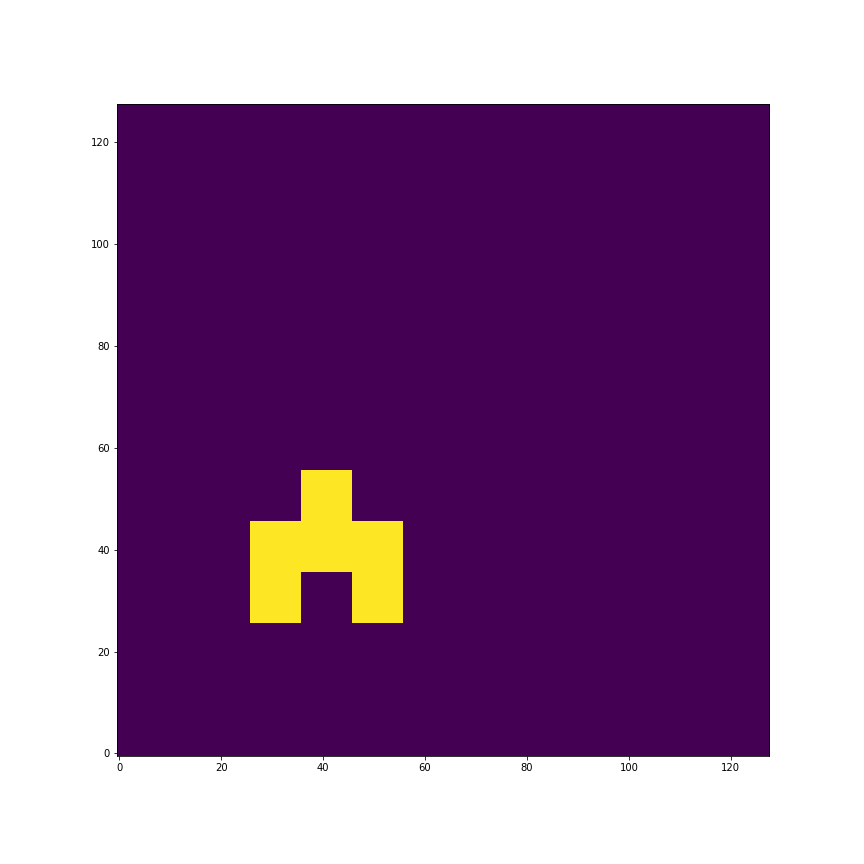
\includegraphics[width=\linewidth]{Pictures/Solve2DWhiteBearMovementTestJR/Solve2DWhiteBearMovementTest_t10.png}
  \captionof{figure}{t=80}
\end{minipage}%
\begin{minipage}{.3\textwidth}
  \centering
  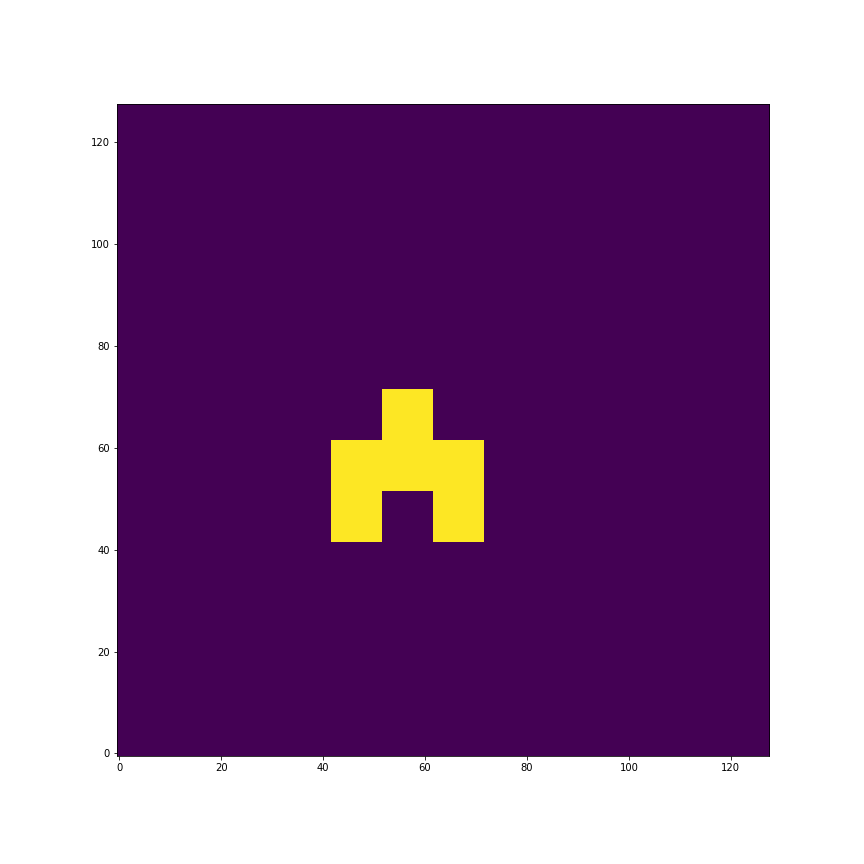
\includegraphics[width=\linewidth]{Pictures/Solve2DWhiteBearMovementTestJR/Solve2DWhiteBearMovementTest_t20.png}
  \captionof{figure}{t=160}
\end{minipage}
\end{figure}

\begin{figure}[H]
\centering
\begin{minipage}{.3\textwidth}
  \centering
  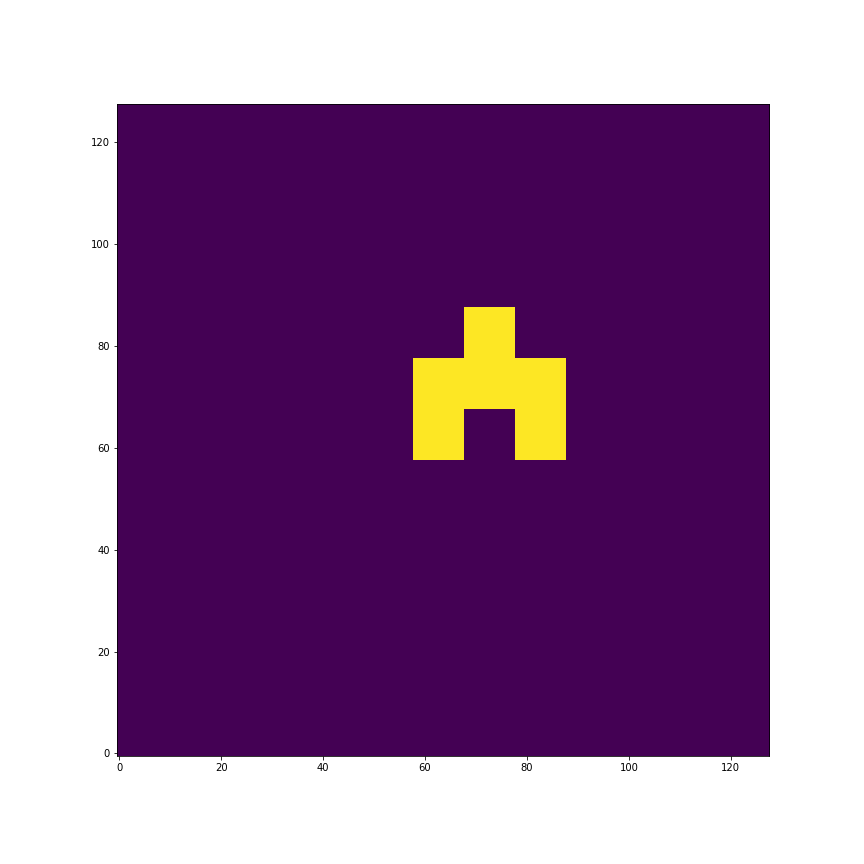
\includegraphics[width=\linewidth]{Pictures/Solve2DWhiteBearMovementTestJR/Solve2DWhiteBearMovementTest_t30.png}
  \captionof{figure}{t=240}
\end{minipage}%
\begin{minipage}{.3\textwidth}
  \centering
  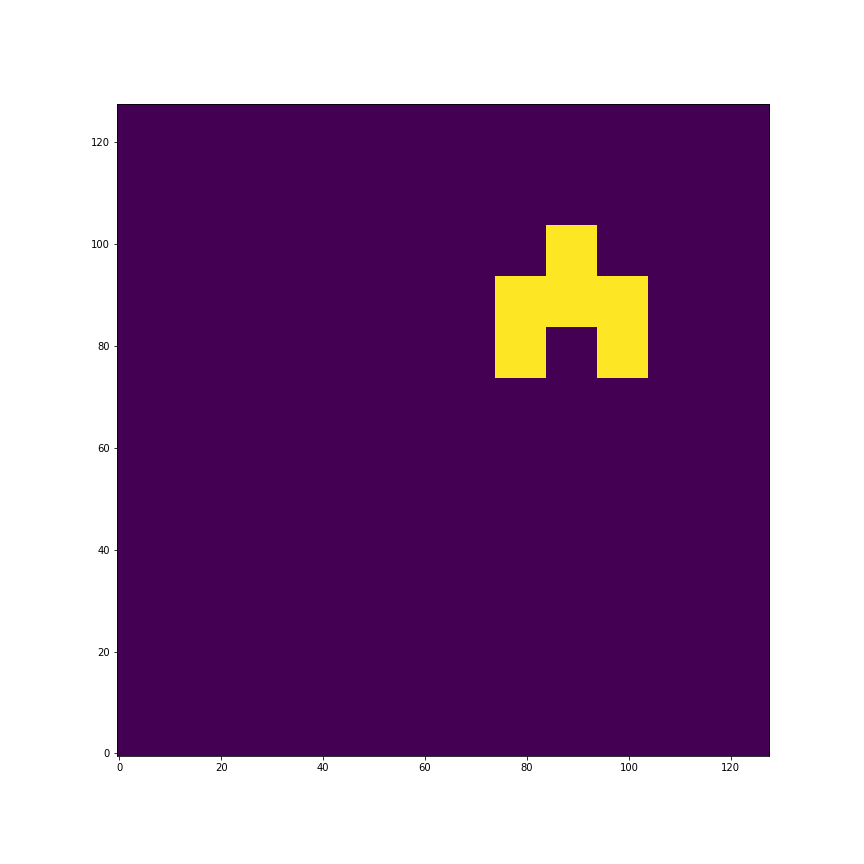
\includegraphics[width=\linewidth]{Pictures/Solve2DWhiteBearMovementTestJR/Solve2DWhiteBearMovementTest_t40.png}
  \captionof{figure}{t=320}
\end{minipage}%
\begin{minipage}{.3\textwidth}
  \centering
  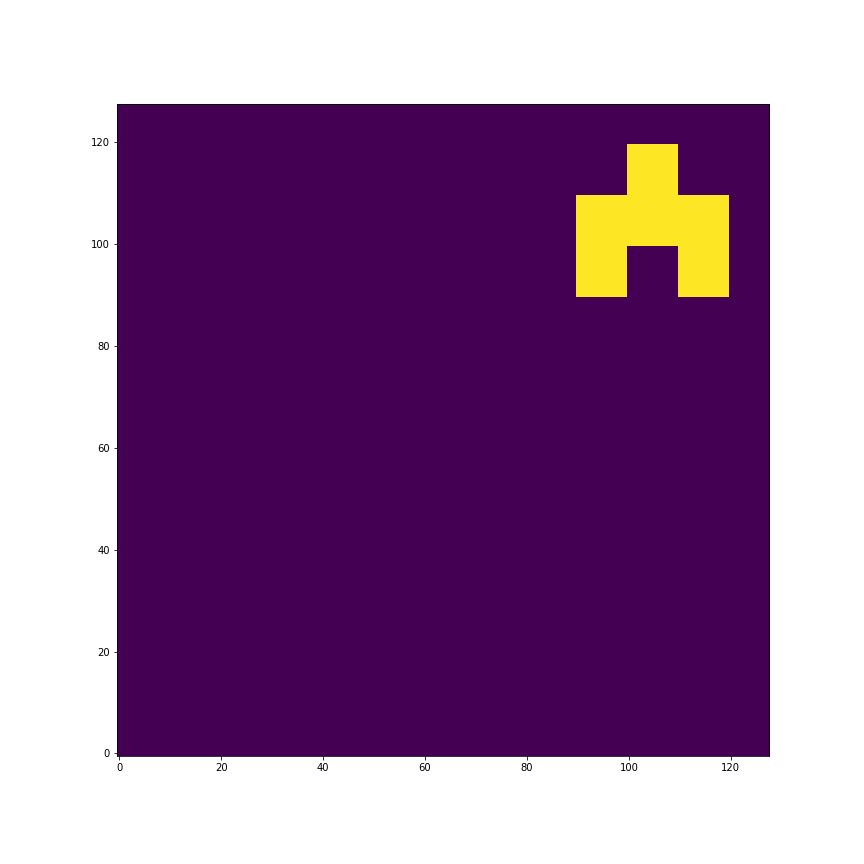
\includegraphics[width=\linewidth]{Pictures/Solve2DWhiteBearMovementTestJR/Solve2DWhiteBearMovementTest_t50.png}
  \captionof{figure}{t=400}
\end{minipage}
\end{figure}

Начальные условия для движения тела в нестационарном поле скорости твердого тела:
\[
\overrightarrow{v}_c(t)=(1, 4-8t)
\]
\[
\overrightarrow{\omega}_c(t)=(0, 0, \pi)
\]
$areaWidth=2.0$\\
$areaHeight=2.0$\\
$cellCountX=128$\\
$cellCountY=128$\\
$NTimeSteps=512$\\

Результаты расчетов для схемы MUSCL:

\begin{figure}[H]
\centering
\begin{minipage}{.3\textwidth}
  \centering
  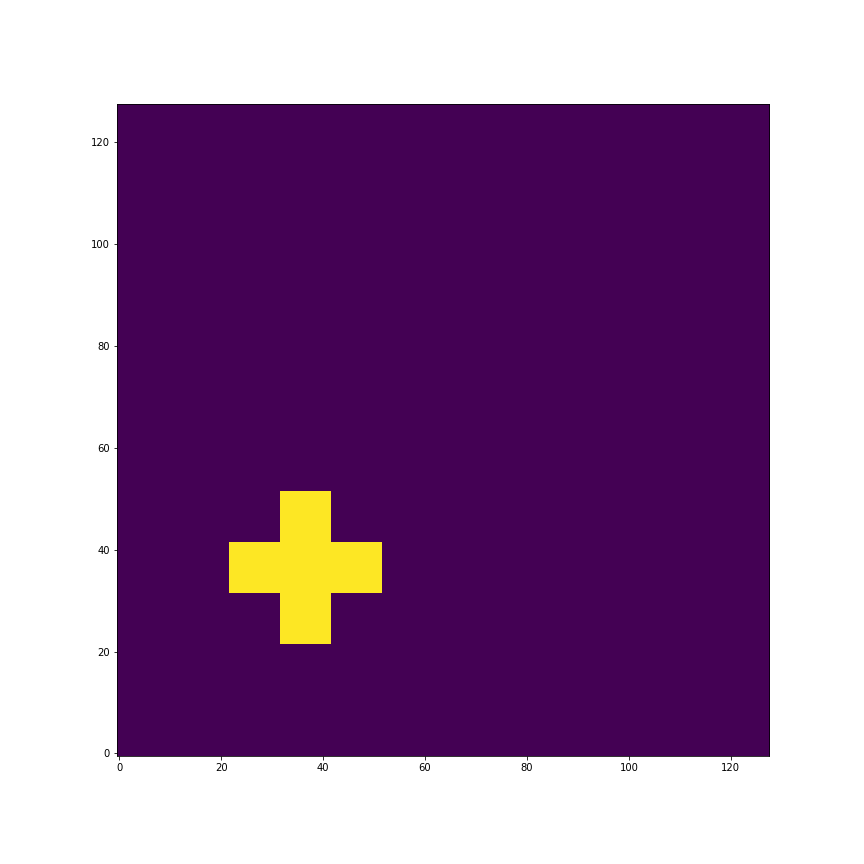
\includegraphics[width=\linewidth]{Pictures/PlusRotateTestMUSCL/PlusRotateTest_t0.png}
  \captionof{figure}{t=0}
\end{minipage}%
\begin{minipage}{.3\textwidth}
  \centering
  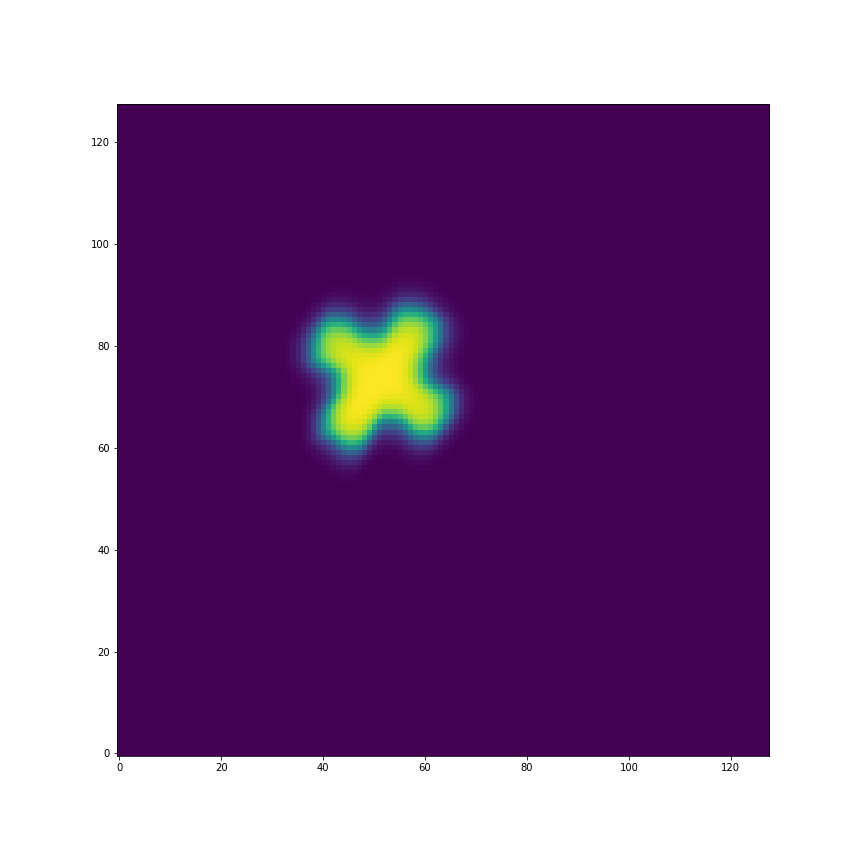
\includegraphics[width=\linewidth]{Pictures/PlusRotateTestMUSCL/PlusRotateTest_t10.png}
  \captionof{figure}{t=102}
\end{minipage}%
\begin{minipage}{.3\textwidth}
  \centering
  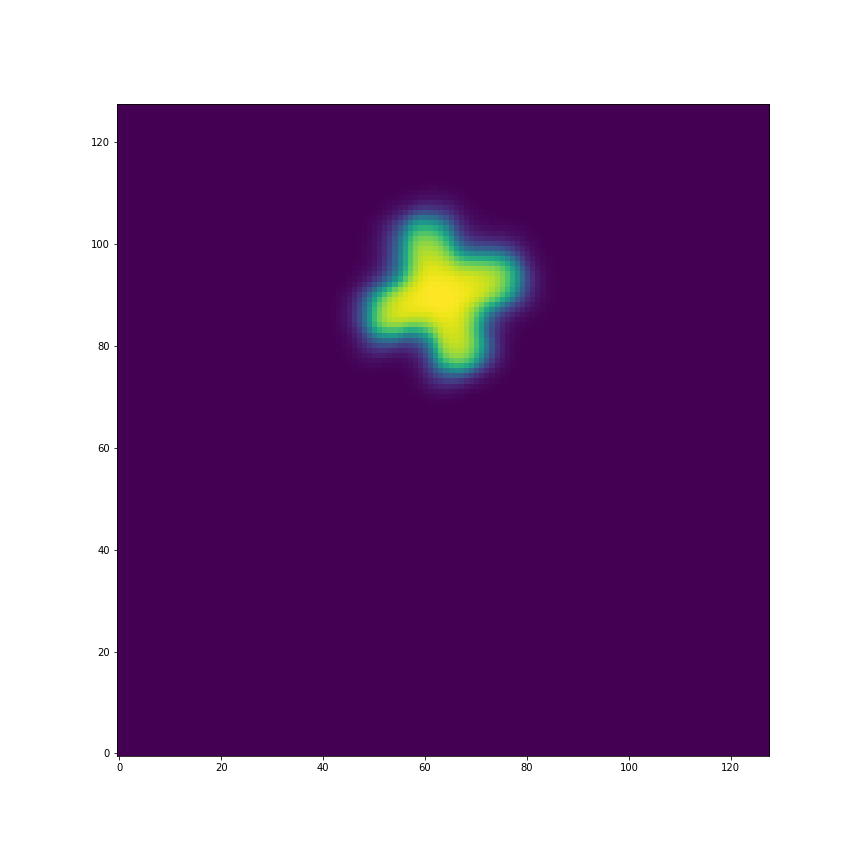
\includegraphics[width=\linewidth]{Pictures/PlusRotateTestMUSCL/PlusRotateTest_t20.png}
  \captionof{figure}{t=205}
\end{minipage}
\end{figure}

\begin{figure}[H]
\centering
\begin{minipage}{.3\textwidth}
  \centering
  \includegraphics[width=\linewidth]{Pictures/PlusRotateTestMUSCL/PlusRotateTest_t30.png}
  \captionof{figure}{t=307}
\end{minipage}%
\begin{minipage}{.3\textwidth}
  \centering
  \includegraphics[width=\linewidth]{Pictures/PlusRotateTestMUSCL/PlusRotateTest_t40.png}
  \captionof{figure}{t=410}
\end{minipage}%
\begin{minipage}{.3\textwidth}
  \centering
  \includegraphics[width=\linewidth]{Pictures/PlusRotateTestMUSCL/PlusRotateTest_t50.png}
  \captionof{figure}{t=512}
\end{minipage}
\end{figure}

Результаты расчетов для схемы THINC:

\begin{figure}[H]
\centering
\begin{minipage}{.3\textwidth}
  \centering
  \includegraphics[width=\linewidth]{Pictures/PlusRotateTestTHINC/PlusRotateTest_t0.png}
  \captionof{figure}{t=0}
\end{minipage}%
\begin{minipage}{.3\textwidth}
  \centering
  \includegraphics[width=\linewidth]{Pictures/PlusRotateTestTHINC/PlusRotateTest_t10.png}
  \captionof{figure}{t=102}
\end{minipage}%
\begin{minipage}{.3\textwidth}
  \centering
  \includegraphics[width=\linewidth]{Pictures/PlusRotateTestTHINC/PlusRotateTest_t20.png}
  \captionof{figure}{t=205}
\end{minipage}
\end{figure}

\begin{figure}[H]
\centering
\begin{minipage}{.3\textwidth}
  \centering
  \includegraphics[width=\linewidth]{Pictures/PlusRotateTestTHINC/PlusRotateTest_t30.png}
  \captionof{figure}{t=307}
\end{minipage}%
\begin{minipage}{.3\textwidth}
  \centering
  \includegraphics[width=\linewidth]{Pictures/PlusRotateTestTHINC/PlusRotateTest_t40.png}
  \captionof{figure}{t=410}
\end{minipage}%
\begin{minipage}{.3\textwidth}
  \centering
  \includegraphics[width=\linewidth]{Pictures/PlusRotateTestTHINC/PlusRotateTest_t50.png}
  \captionof{figure}{t=512}
\end{minipage}
\end{figure}

Результаты расчетов для схемы JR:

\begin{figure}[H]
\centering
\begin{minipage}{.3\textwidth}
  \centering
  \includegraphics[width=\linewidth]{Pictures/PlusRotateTestJR/PlusRotateTest_t0.png}
  \captionof{figure}{t=0}
\end{minipage}%
\begin{minipage}{.3\textwidth}
  \centering
  \includegraphics[width=\linewidth]{Pictures/PlusRotateTestJR/PlusRotateTest_t10.png}
  \captionof{figure}{t=102}
\end{minipage}%
\begin{minipage}{.3\textwidth}
  \centering
  \includegraphics[width=\linewidth]{Pictures/PlusRotateTestJR/PlusRotateTest_t20.png}
  \captionof{figure}{t=205}
\end{minipage}
\end{figure}

\begin{figure}[H]
\centering
\begin{minipage}{.3\textwidth}
  \centering
  \includegraphics[width=\linewidth]{Pictures/PlusRotateTestJR/PlusRotateTest_t30.png}
  \captionof{figure}{t=307}
\end{minipage}%
\begin{minipage}{.3\textwidth}
  \centering
  \includegraphics[width=\linewidth]{Pictures/PlusRotateTestJR/PlusRotateTest_t40.png}
  \captionof{figure}{t=410}
\end{minipage}%
\begin{minipage}{.3\textwidth}
  \centering
  \includegraphics[width=\linewidth]{Pictures/PlusRotateTestJR/PlusRotateTest_t50.png}
  \captionof{figure}{t=512}
\end{minipage}
\end{figure}

Сравнение размазывания исходной формы твердого тела после поступательного и вращательного движения:
\begin{figure}[H]
\centering
\begin{minipage}{.25\textwidth}
  \centering
  \includegraphics[width=\linewidth]{Pictures/PlusInit.png}
  \captionof{figure}{Initial}
\end{minipage}%
\begin{minipage}{.25\textwidth}
  \centering
  \includegraphics[width=\linewidth]{Pictures/PlusMUSCL.png}
  \captionof{figure}{MUSCL}
\end{minipage}%
\begin{minipage}{.25\textwidth}
  \centering
  \includegraphics[width=\linewidth]{Pictures/PlusTHINC.png}
  \captionof{figure}{THINC}
\end{minipage}%
\begin{minipage}{.25\textwidth}
  \centering
  \includegraphics[width=\linewidth]{Pictures/PlusJR.png}
  \captionof{figure}{JR}
\end{minipage}
\end{figure}

\newpage
\section{Заключение}
Были исследованы численные методы решения уравнения переноса и реализован его программный алгоритм для одномерного случая.

Исследование схем для решения уравнение переноса в одномерном случае позволяет использовать данный подход в двумерном и трехмерном пространстве методом расщепления по координатным направлениям. Программа, написанная для одномерного случая, используется в дальнейшем как расчетный блок для многомерного случая.

Для представления цифровой геометрии были исследованы схемы с разным порядком точности, в том числе схема Годунова, MUSCL и THINC. Применение схемы THINC в отличие от других схем позволяет с высокой точностью описать поведение геометрии в цифровом виде, значительно уменьшить величину ошибки при расчетах.

Был разработан метод точного восполнения разрыва характеристической функции на подсеточном уровне (Jump Reconstruction, JR). Метод Jump Reconstruction позволяет в точности восстановить решение в одномерном случае и показывает хорошие результаты при многомерном обобщении.

\newpage
\begin{thebibliography}{3}
\bibitem{Godunov_sovle_gido}Годунов С.К. О единственности решения уравнений гидродинамики / С.К.Годунов // Математический сборник. - 1956. - Т.40, N 4. - С.467-478.
\bibitem{Godunov_diff_scheme}Багриновский К.А. Разностные схемы для многомерных задач / К.А.Багриновский, С.К.Годунов // Доклады Академии наук СССР. - 1957. - Т.115, N 3. - С.431-433.
\bibitem{Godunov_num_method}Годунов С.К. Разностный метод численного расчета разрывных решений уравнений гидродинамики / С.К.Годунов // Математический сборник. - 1959. - Т.47, N 3. - С.271-306.
\bibitem{Godunov_smearing}Годунов С.К. О неединственном «размазывании» разрывов в решениях квазилинейных систем / С.К.Годунов // Доклады Академии наук СССР. - 1961. - Т.136, N 2. - С.272-273.
\bibitem{Godunov_error}Годунов С.К. Оценки невязок для приближенных решений простейших уравнений газовой динамики / С.К.Годунов // Журнал вычислительной математики и математической физики. - 1961. - Т.1, N 4. - С.622-637.
\bibitem{Godunov_num_sch_2nd_ord}Годунов С.К. О разностных схемах второго порядка точности для многомерных задач / С.К.Годунов, А.В.Забродин // Журнал вычислительной математики и математической физики. - 1962. - Т.2, N 4. - С.706-708.
\bibitem{Godunov_num_method_2}Годунов С.К. Разностные методы численного решения задач газовой динамики / С.К.Годунов, К.А.Семендяев // Журнал вычислительной математики и математической физики. - 1962. - Т.2, N 1. - С.3-14.
\bibitem{bib_item}Годунов С.К. Проблема обобщенного решения в теории квазилинейных уравнений и в газовой динамике / С.К.Годунов // Успехи математических наук. - 1962. - Т.17, вып.3. - С.147-158.
\bibitem{bib_item}Годунов С.К. Об использовании подвижных сеток в газодинамических расчетах / С.К.Годунов, Г.П.Прокопов // Журнал вычислительной математики и математической физики. - 1972. - Т.12, N 2. - С.429-440.
\bibitem{bib_item}Бахвалов П.А. Нестационарный метод геометрического корректора и его использование для оценки точности конечно-объемной схемы на неструктурированных сетках // Препринты ИПМ им. М.В.Келдыша. - 2016. - № 122. - 28 с.
\bibitem{MUSCL_Bochkarev}Бочкарева Е.В., Храпов С.С. Численное моделирование динамики звуковых волн в активных средах с использованием схемы MUSCL // Вестник Волгоградского государственного университета. Серия 1: Математика. Физика. – 2015. – № 1 (18). - С. 13-22.
\bibitem{MUSCL_Kostushin}К. В. Костюшин, В. А. Шувариков, Сравнение схем типа "MUSCL" для расчета течений идеального газа в соплах
Лаваля, Вестн. Томск. гос. ун-та. Матем. и мех., 2018.
\bibitem{bib_item}Чжан Ч., Меньшов И.С. Сквозной метод расчета уравнений переноса многокомпонентной гетерогенной системы на фиксированных эйлеровых сетках // Математическое моделирование. – 2019. - №4 (31). – С. 111–130.
\bibitem{THINC_Xiao}Xiao F., Honma Y., Kono T. A simple algebraic interface capturing scheme using hyperbolic tangent function // International Journal for Numerical Methods in Fluids. 2005. Т. 48, № 9, с. 1023—1040.
\bibitem{bib_item}Einfeldt B., Munz C. D., Roe P. L. On Godunov-type methods near low densities // Journal of Computational Physics. 1991. Т. 92, № 2, с. 273—295.
\bibitem{THINC_Kumar}Ronit Kumar, Lidong Cheng, Yunong Xiong, Bin Xie, Rémi Abgrall, Feng Xiao. THINC scaling method that bridges VOF and level set schemes. // Journal of Computational Physics. 2021. 436: 110323.
\end{thebibliography}

\newpage
\section{Приложения}
\subsection{Пример программного кода нахождения координаты центра твердого тела в моменты времени $t_i$}
\label{code:xc}
\begin{lstlisting}
function<Vector2D(vector<Vector2D>, double)> trapezoidQuadrature(){
    return [&](vector<Vector2D> f, double dx) -> Vector2D {
        return (f[0]+f[1])/2.*dx;
    };
}

void EESolver2DCenterStep(Vector2D& xc, const vector<Vector2D>& vc, int it,
const EESolver2DParams& params){
    if(it<=0) return;
    xc+=trapezoidQuadrature()({vc[it-1], vc[it]}, params.getDt());
}

void SolveEE2D(vector<Vector2D>& vertices, //vertices[0] is center
               const vector<Vector2D>& vc, const vector<double>& w,
               const EESolver2DParams& params, EESolver2DOutput& out){
    out.print(vertices, 0);
    for(int it=1; it<=params.getNTimeSteps(); it++){
        EESolver2DCenterStep(vertices[0], vc, it, params);
        //TODO solve for vertices here
        out.print(vertices, it);
    }
}
\end{lstlisting}

\subsection{Пример программного кода нахождения значений правой функции в моменты времени $t_i$}
\label{code:rf}
\begin{lstlisting}
Array<VectorXd, Dynamic, 1> integrateVector(Array<VectorXd, Dynamic, 1> f, double a, double b) {
    Array<VectorXd, Dynamic, 1> integral(f.size());
    double h = (b - a) / (f.size() - 1.);
    VectorXd i0 = VectorXd::Zero(f(0).size());
    integral(0) = i0;
    for (int i = 1; i < f.size(); i++) {
        integral(i) = integral(i - 1);
        integral(i) += (f(i - 1) + f(i)) * h / 2;
    }
    return integral;
}

function<VectorXd(double)> getRightFunc(function<VectorXd(double)> v, VectorXd xi0, function<Vector3d(double)> omega, function<VectorXd(double)> xc) {
    return [=](double t)->VectorXd {
        function<VectorXd(double)> integrand = [=](double tau)->VectorXd {
            VectorXd xcTau = xc(tau);
            Vector3d xcTau3(xcTau(0), xcTau(1), dimN < 3 ? 0 : xcTau(2));
            Vector3d crossProd = xcTau3.cross(omega(tau));
            VectorXd crossProdX(dimN);
            for (int i = 0; i < dimN; i++) crossProdX(i) = crossProd(i);
            return v(tau) - crossProdX;
        };
        return xi0 + integrateVector(integrand, 0, t, pow(10, -5), pow(10, -5));
    };
}

function<VectorXd(double)> getRightFuncNoMargin(function<VectorXd(double)> v, function<Vector3d(double)> omega, function<VectorXd(double)> xc) {
    return [=](double t)->VectorXd {
        function<VectorXd(double)> integrand = [=](double tau)->VectorXd {
            VectorXd xcTau = xc(tau);
            Vector3d xcTau3(xcTau(0), xcTau(1), dimN < 3 ? 0 : xcTau(2));
            Vector3d crossProd = xcTau3.cross(omega(tau));
            VectorXd crossProdX(dimN);
            for (int i = 0; i < dimN; i++) crossProdX(i) = crossProd(i);
            return v(tau) - crossProdX;
        };
        return integrateVector(integrand, 0, t, pow(10, -5), pow(10, -5));
    };
}
\end{lstlisting}

\subsection{Пример программного кода нахождения значений $x_k^i$}
\label{code:xk}
\begin{lstlisting}
Array<VectorXd, Dynamic, 1> getXi(function<VectorXd(double)> v,
VectorXd xi0,
function<Vector3d(double)> omega,
function<VectorXd(double)> xc, int stepsN, double h) {

    Array<VectorXd, Dynamic, 1> Xn(stepsN + 1);

    Array<VectorXd, Dynamic, 1> rightFuncCalc(stepsN + 1);
    function<VectorXd(double)> rightFunc = getRightFunc(v, xi0, omega, xc);
    for (int i = 0; i <= stepsN; i++)
        rightFuncCalc(i) = rightFunc(i * h);

    cout << "rightFuncCalc calculated" << endl;

    Xn(0) = rightFuncCalc(0);

    for (int k = 1; k <= stepsN; k++) {
        double sk = k * h;

        VectorXd innerSum(dimN);
        for (int i = 0; i < dimN; i++) innerSum(i) = 0;


        for (int j = 0; j < k; j++) {
            double sj = j * h;
            double Aj = (j == 0 ? 1. / 2. : 1.);

            VectorXd prodResult(dimN);
            Vector3d Xj(Xn(j)(0), Xn(j)(1), dimN < 3 ? 0 : Xn(j)(2));
            Vector3d crossProd = Xj.cross(omega(sj));
            for (int i = 0; i < dimN; i++) prodResult(i) = crossProd(i);

            innerSum += Aj * prodResult;
        }

        // Xk - h * innerSum(K-1) - h * Ak * [Xk ; OmegaK]  = rightFuncK
        // Xk - [Xk ; h * Ak *  OmegaK]  = rightFuncK + h * innerSum(K-1)
        // a - [a ; b] = c, a=?
        // ax - ay*bz = cx
        // ay + ax*bz = cy
        // (1 -bz)(ax)=(cx)
        // (bz  1)(ay)=(cy)
        // Ba=c, a = invB c

        Vector3d b = h * 0.5 * omega(sk);

        Vector2d rf2(rightFuncCalc(k)(0), rightFuncCalc(k)(1));
        Vector2d is2(innerSum(0), innerSum(1));
        Vector2d c = rf2 + h * is2;

        Matrix2d B; B <<
            1, -b(2),
            b(2), 1;

        Vector2d a = B.inverse() * c;

        VectorXd Xk(dimN);
        for (int i = 0; i < dimN; i++) Xk(i) = a(i);

        Xn(k) = Xk;
    }

    return Xn;

}
\end{lstlisting}

\subsection{Пример программного кода решения уравнения переноса в одномерном случае со стационарным полем скоростей}
\label{code:TESolver1D}
\begin{lstlisting}
double flow(const function<double(double)>& PsyL,
            const function<double(double)>& PsyR,
            double x, double u, double dt){
    return u>=0 ?
    PsyL(getXforInterpolation(x, u, dt/2)) :
    PsyR(getXforInterpolation(x, u, dt/2));
}

double fNext(F1D fi,
             U1D ui,
             C1D ci,
             double dt,
             const vector<function<double(double)>> &Psy){ // 3 functions: {Psy|i-1 , Psy|i , Psy|i+1}
    double fiR = flow(Psy[1], Psy[2], ci.xR, ui.uR, dt);
    double fiL = flow(Psy[0], Psy[1], ci.xL, ui.uL, dt);
    return fi.fi - 1.0 / ci.dx * (fiR*ui.uR - fiL*ui.uL) * dt;
}

void TESolverStep(LineInterface &f,
                  LineInterface &u,
                  TESolver1DParams &p){
    vector<function<double(double)>> Psy(p.getCellCount()+2);
    for(int i=-1; i<p.getCellCount()+1; i++){
        int sgnUi = 0;
        if(i==-1) //TODO extend u outside area like f
            sgnUi = sgn(u[0]);
        else if(i==p.getCellCount())
            sgnUi = sgn(u[i]);
        else
            sgnUi = sgn((u[i]+u[i+1])/2.);
        F1D fi = getFi(f, i);
        C1D ci = getCi(p.getDx(), i);
        if(sgnUi<0){
            F1D invFi = inverse(fi);
            C1D invCi = inverse(ci);
            Psy[i+1] = fInverseX(p.getFlowInterpolationFunctionBuilder()(invFi, invCi));
        } else {
            Psy[i+1] = p.getFlowInterpolationFunctionBuilder()(fi, ci);
        }
    }


    double fiPrev = f[-1];
    double fiAfterLast = f[p.getCellCount()];

    for (int i = 0; i < p.getCellCount()-1; i++) { // calculating all cells except last
        F1D fi = getFi(f, i);
        fi.fiPrev = fiPrev; // using saved fi as fiPrev in the next cell
        fiPrev = fi.fi;
        f.set(i, fNext(fi, getUi(u, i), getCi(p.getDx(), i), p.getDt(),
                       {Psy[i], Psy[i+1], Psy[i+2]}));
    }
    // fiNext for last cell is old f0, so we calc this separately
    int iLast = p.getCellCount()-1;
    F1D fiLast = {f[iLast], fiPrev, fiAfterLast};
    f.set(iLast, fNext(fiLast, getUi(u, iLast), getCi(p.getDx(), iLast), p.getDt(), {Psy[iLast], Psy[iLast+1], Psy[iLast+2]}));
}

void SolveTransportEquation1D(Area1D &f,
                              VectorField1D &u,
                              TESolver1DParams &p,
                              TESolver1DOutput &output) {
    output.print(f, 0, p.getDx());
    for (int n = 0; n < p.getNTimeSteps(); n++) {
        TESolverStep(f, u, p);
        output.print(f, n+1, p.getDx());
    }
}
\end{lstlisting}

\end{document}